%-------------------------------------------------------------------------------
%                            BAB IV
%               		HASIL DAN PEMBAHASAN
%-------------------------------------------------------------------------------
% \fancyhf{} 
% \fancyfoot[R]{\thepage}
\chapter{HASIL DAN PEMBAHASAN}
%\thispagestyle{plain} % Halaman pertama bab menggunakan gaya plain

\section{Hasil Survei Kuesioner Petani di Kabupaten Aceh Besar}
Pengumpulan data lapangan dilakukan melalui survei kuesioner, melibatkan 50 petani tersebar di tiga kecamatan, yaitu Indrapuri, Montasik, dan Darussalam. Proses wawancara dan pengisian kuesioner di lapangan secara langsung dilaksanakan oleh tim lain, sementara penulis dan dua anggota lainnya bertanggung jawab pada tahap rekapitulasi, validasi, dan digitalisasi data hasil survei ke dalam sistem. Informasi tersebut menjadi dasar untuk memahami kebutuhan informasi iklim serta relevansi sistem yang dikembangkan..
% Penelitian ini diawali dengan pengumpulan data kuesioner yang melibatkan petani untuk memetakan kondisi awal pertanian di Kabupaten Aceh Besar seperti yang ditampilkan pada gambar \ref{fig:responden_petani}.
% \begin{figure}[H]
%     \centering
%     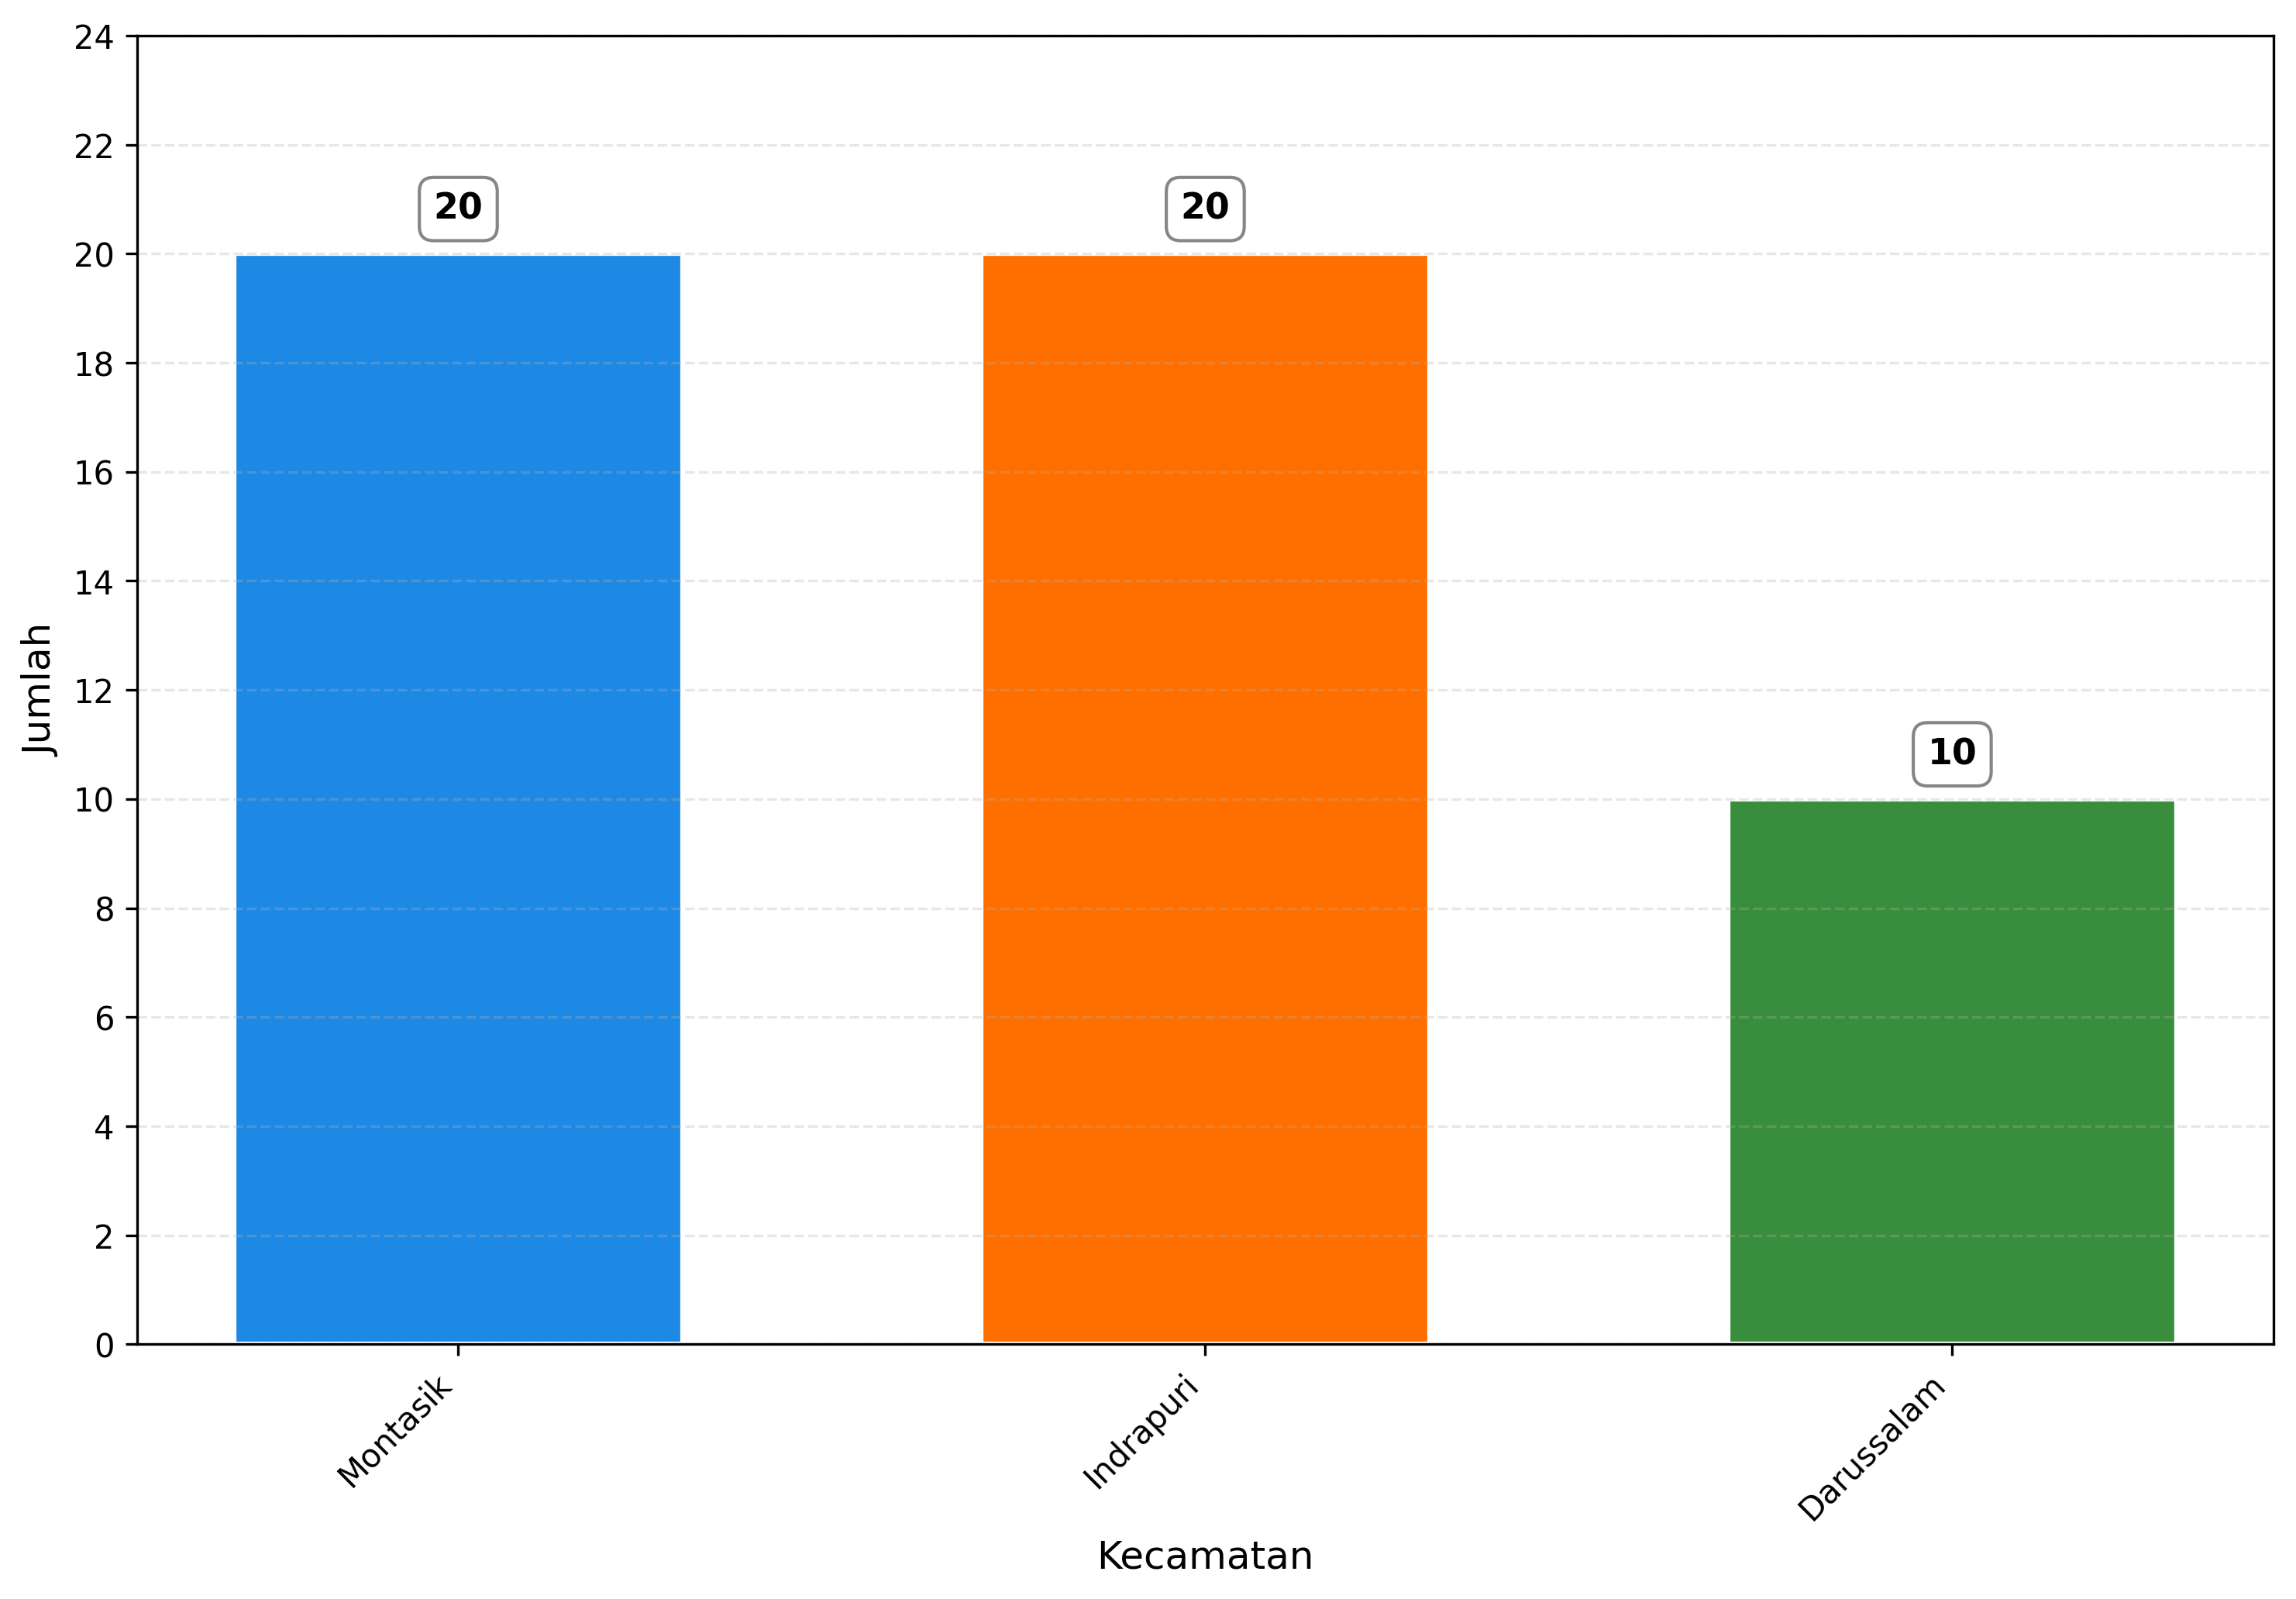
\includegraphics[width=0.8\linewidth]{image/bab4/01_responden_aceh_besar_per_kecamatan.png}
%     \caption{Distribusi Responden Petani per Kecamatan di Kabupaten Aceh Besar}
%     \label{fig:responden_petani}
% \end{figure}
% Berdasarkan Gambar \ref{fig:responden_petani} diatas, responden berjumlah 50 petani berasal dari 3 kecamatan di mana 20 petani berasal dari kecamatan Indrapuri, 20 petani berasal dari kecamatan Montasik, dan 10 petani berasal dari kecamatan Darussalam. Melalui kuesioner ini, diperoleh data empiris mengenai praktik pertanian lokal yang meliputi jenis bibit, Jenis lahan, dan siklus tanam maupun panen setiap musim.
\begin{figure}[H]
    \centering
    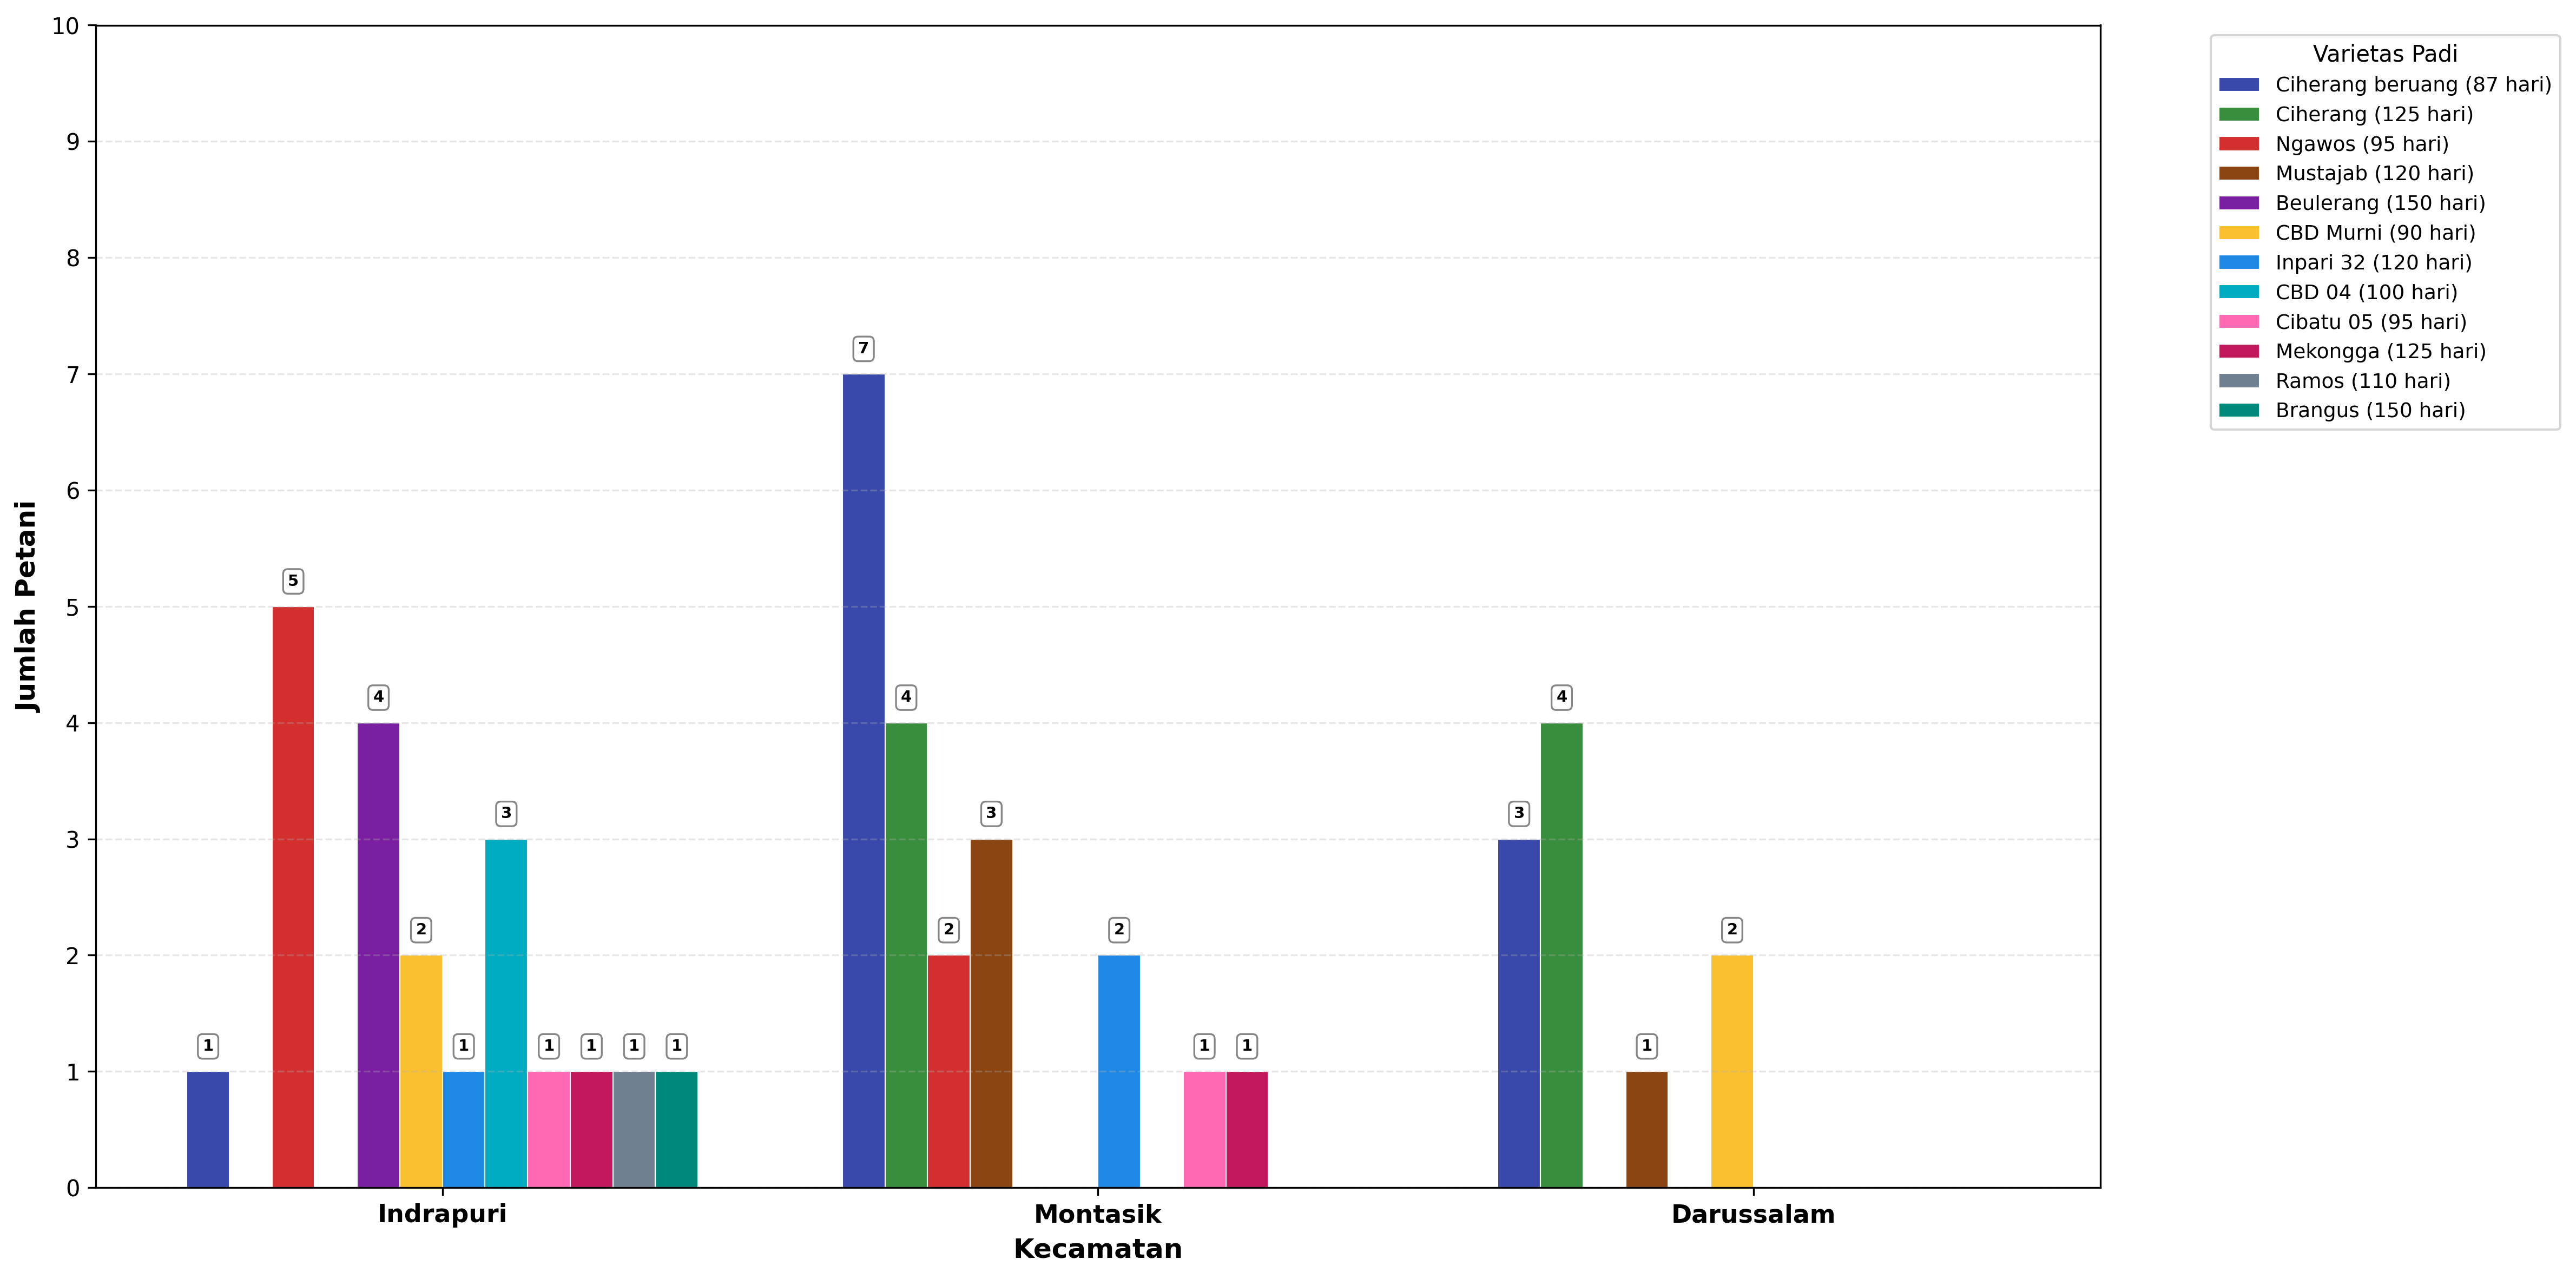
\includegraphics[width=0.8\linewidth]{image/bab4/02_varietas_padi_per_kecamatan_aceh_besar.png}
    \caption{Varietas Padi di Kabupaten Aceh Besar}
    \label{fig:varietas_padi}
\end{figure}
Gambar \ref{fig:varietas_padi} menunjukkan bahwa jenis bibit padi di Kabupaten Aceh Besar antara lain Ciherang Beruang (15 petani), Ngawos (7 petani), Beulerang (4 petani), Ciherang (3 petani), Inpari 32 (3 petani), Mustajab (3 petani), CBD 04 (3 petani), Cibatu 05 (2 petani), Mekongga (2 petani), CBD Murni (2 petani), Ramos (1 petani), dan Brangus (1 petani), dengan durasi tanam berkisar antara 87 hingga 150 hari. Pemilihan bibit ini berkaitan erat dengan ketersediaan air irigasi dan pola musiman.
\begin{figure}[H]
    \centering
    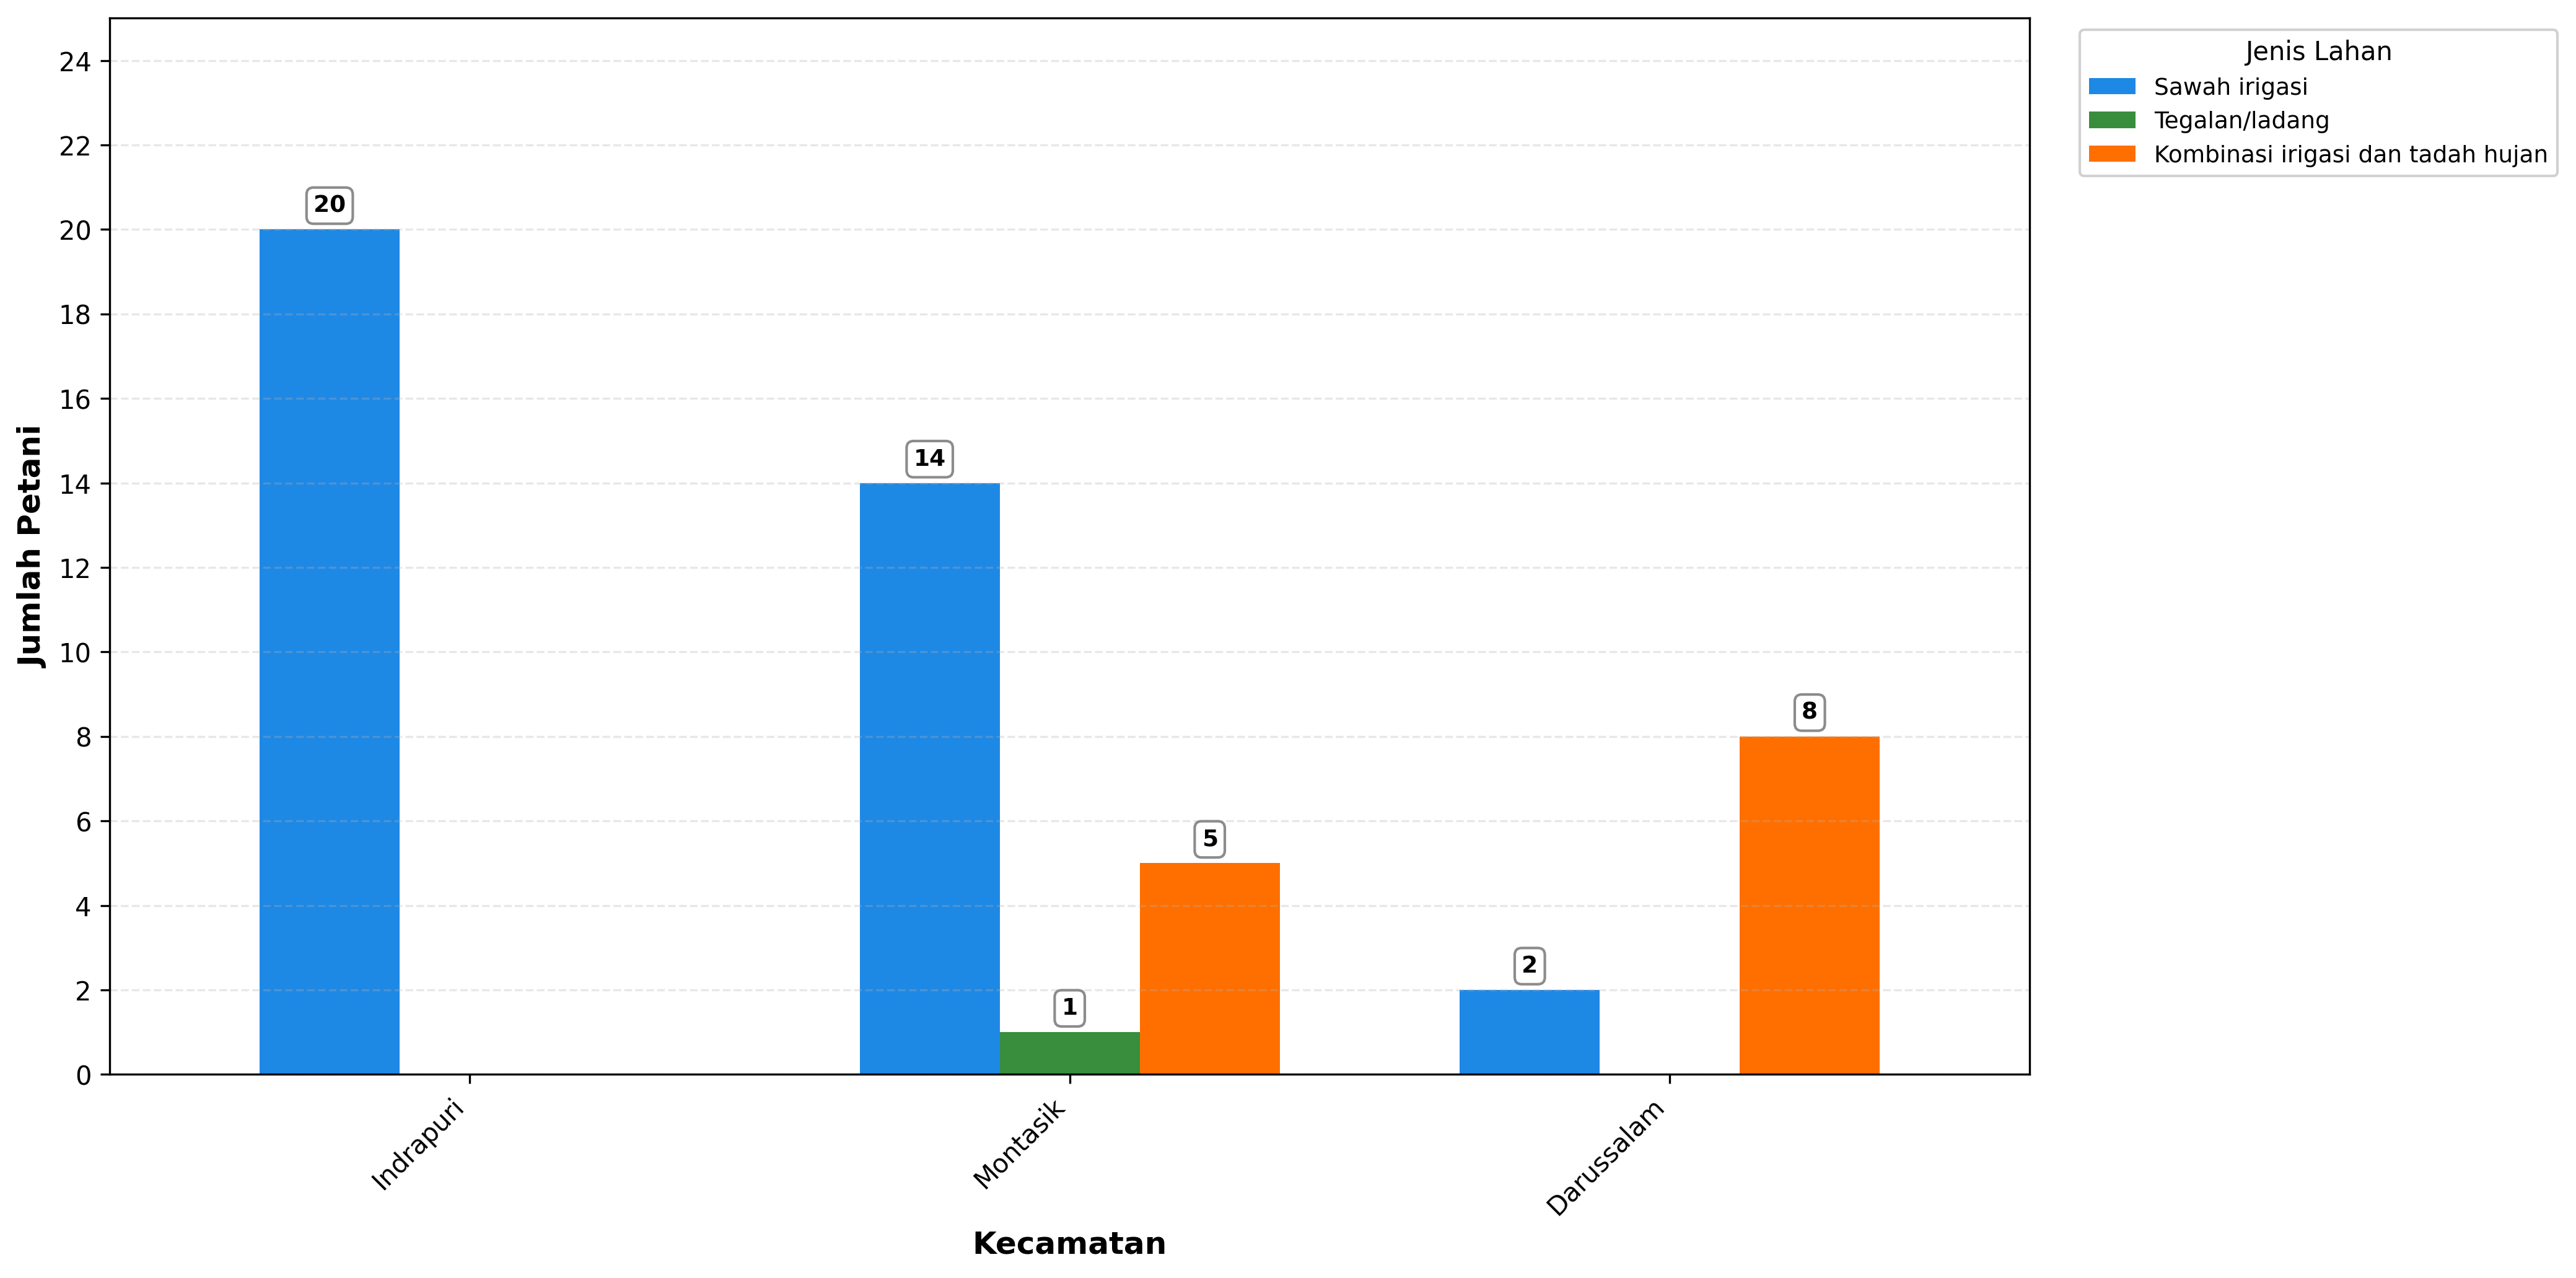
\includegraphics[width=0.8\linewidth]{image/bab4/03_distribusi_jenis_lahan_kecamatan_aceh_besar.png}
    \caption{Jenis Lahan Pertanian Kabupaten Aceh Besar}
    \label{fig:jenis_lahan}
\end{figure}
Adapun jumlah periode tanam di Kabupaten Aceh Besar memperlihatkan pola musiman yang berbeda antar kecamatan. Berdasarkan Gambar \ref{fig:jenis_lahan}, Di Montasik, aktivitas tanam paling dominan terjadi pada bulan Mei–Juli dengan 18 periode, disusul November–Januari sebanyak 16 periode, sementara Februari–April dan Agustus–Oktober relatif kecil dengan masing-masing 2 periode. Pola serupa terlihat di Indrapuri, di mana petani banyak menanam pada Mei–Juli dan November–Januari (masing-masing 15 periode), sedangkan Februari–April dan Agustus–Oktober hanya tercatat 3 periode. Adapun di Darussalam, kegiatan tanam lebih terbatas, dengan konsentrasi pada November–Januari sebanyak 12 periode dan sedikit aktivitas pada Mei–Juli (1 periode). Secara keseluruhan, mayoritas petani di Aceh Besar melakukan dua kali tanam dalam setahun, terutama pada musim hujan dan awal musim kemarau.
\begin{figure}[H]
    \centering
    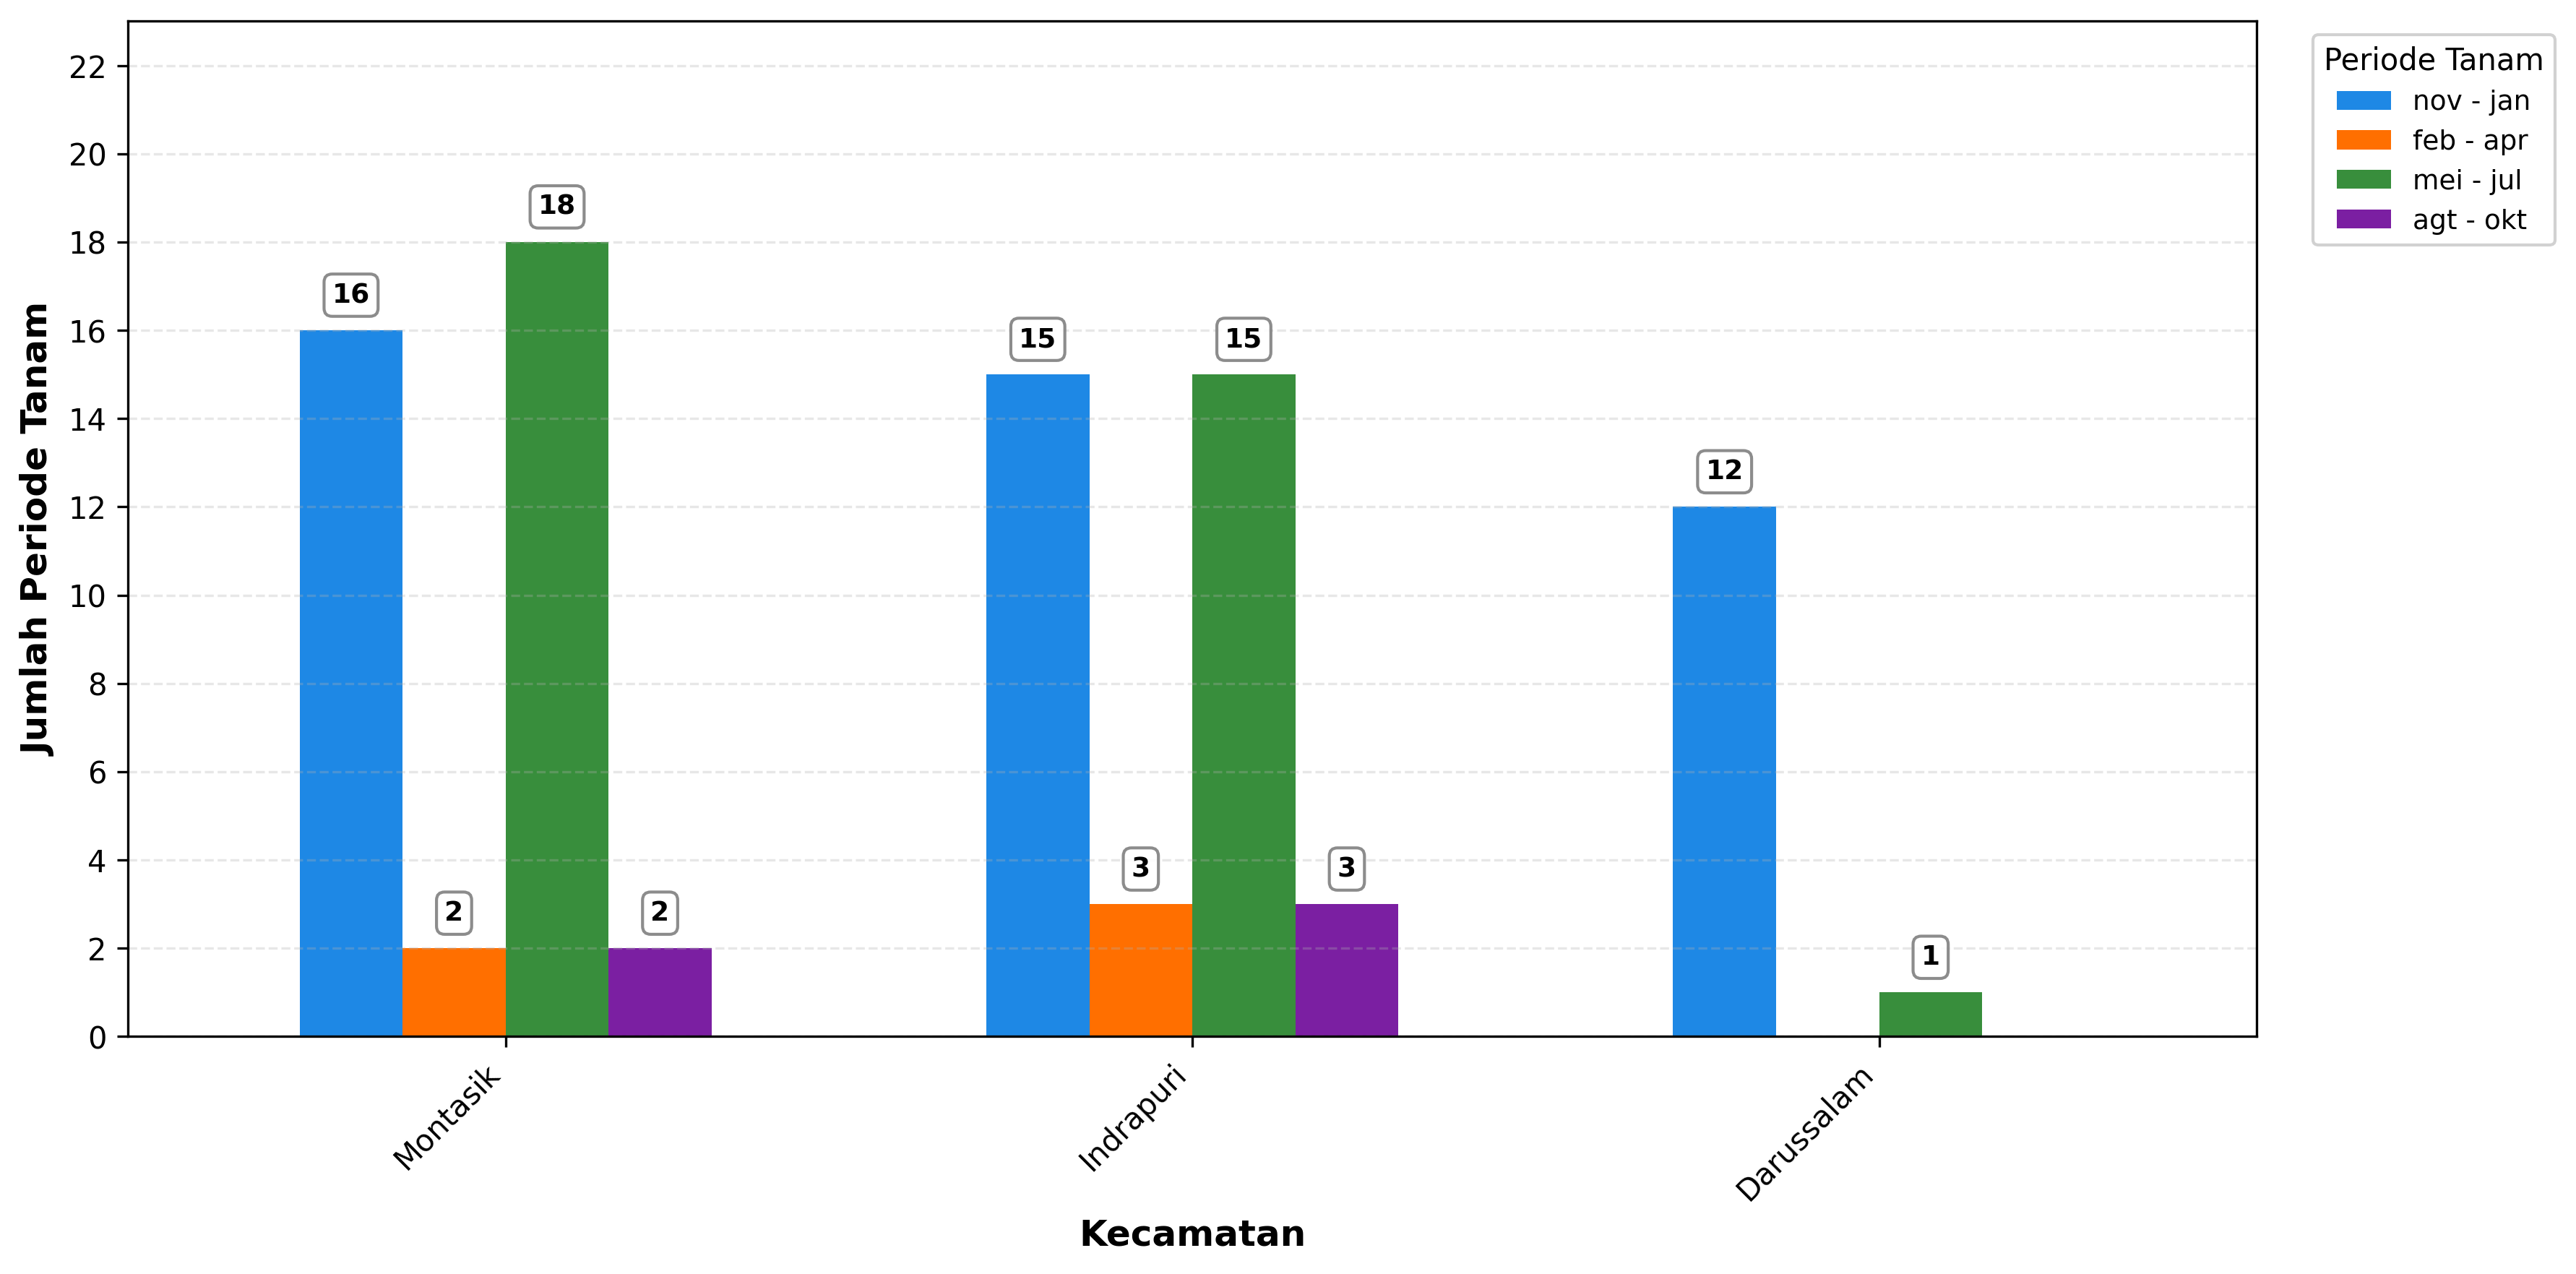
\includegraphics[width=0.8\linewidth]{image/bab4/04_distribusi_periode_tanam_kecamatan.png}
    \caption{Periode Tanam di Kabupaten Aceh Besar}
    \label{fig:periode_tanam}
\end{figure}
Gambar \ref{fig:periode_tanam} di atas menunjukkan variasi periode tanam di tiga kecamatan. Pada Kecamatan Montasik, aktivitas tanam paling banyak terjadi pada bulan Mei–Juli (18 periode) dan November–Januari (16 periode), sementara Februari–April dan Agustus–Oktober hanya tercatat masing-masing 2 periode. Pola serupa terlihat di Indrapuri, di mana petani menanam terutama pada Mei–Juli dan November–Januari (masing-masing 15 periode), sedangkan Februari–April dan Agustus–Oktober relatif kecil dengan 3 periode. Adapun di Kecamatan Darussalam, kegiatan tanam lebih terbatas, dengan konsentrasi pada November–Januari sebanyak 12 periode dan hanya 1 periode pada Mei–Juli. Secara keseluruhan, data ini memperlihatkan bahwa mayoritas petani di Aceh Besar melakukan dua kali tanam dalam setahun, dengan fokus pada musim hujan dan awal musim kemarau sebagai bentuk adaptasi terhadap ketersediaan air dan kondisi iklim setempat.

% dengan rentang pengambilan data selama 20 tahun atau 7578 observasi mulai dari 1 Januari 2005 hingga 30 September 2025.

\section{Implementasi}
Sistem Otomasi Pemrosesan Data Iklim dengan Metode \textit{smoothing} telah di implementasikan menggunakan \textit{framework} Next.js (\textit{frontend}) dan Flask (\textit{backend}), dengan \textit{database} MongoDB. Proses implementasi dilakukan secara bertahap mengikuti alur pengembangan Agile yang telah dirancang sebelumnya \ref{pembagian_sprint}. Pengembangan dibagi menjadi lima sprint dengan durasi masing-masing 2–4 minggu.

Sprint pertama difokuskan pada analisis kebutuhan, perancangan skema \textit{database}, serta identifikasi sumber data iklim (BMKG dan NASA POWER). Sprint kedua mengimplementasikan \textit{frontend} berbasis Next.js, meliputi halaman \textit{dashboard} untuk memantau status \textit{dataset}, upload data, dan visualisasi data. Sprint ketiga mengembangkan \textit{backend} dengan Flask, mencakup pembuatan REST API untuk \textit{data acquisition}, serta integrasi ke MongoDB. Sprint keempat mengimplementasikan \textit{pipeline preprocessing} data BMKG dan NASA POWER, termasuk metode \textit{smoothing} (imputasi nilai hilang, \textit{outlier detection}, \textit{exponential smoothing}, dan validasi kualitas dengan GCV). Sprint kelima melakukan pengujian menyeluruh (API integration testing, data testing, dan pengujian otomasi scheduler) serta \textit{deployment} sistem ke \textit{production}.

\subsection{Implementasi \textit{frontend}}
Implementasi \textit{frontend} difokuskan pada manajemen dashboard \textit{dashboard} yang hanya dapat diakses oleh \textit{role} admin. Berikut adalah beberapa tampilan utama:
\begin{enumerate}[(a)]
\item \textbf{Halaman \textit{dashboard}}: Admin melakukan manajemen \textit{dataset} di dalam sistem.
        \begin{figure}[H]
            \centering
            
\includegraphics[width=0.95\linewidth]{image/bab4/halaman_dashboard.png}
            \caption{Halaman \textit{Dashboard}}
            \label{fig:halaman_dashboard}
        \end{figure}
        Gambar \ref{fig:halaman_dashboard} menampikan halaman \textit{dashboard} utama yang berisi daftar \textit{dataset} yang digunakan oleh sistem. Terdapat menu di sebelah kiri untuk navigasi ke fitur lainnya seperti Halaman \textit{Reports}, Halaman Otomasi, Kalender Tanam, Data Bibit, dan Recyle Bin. Terdapat \textit{filter} di sebelah kanan untuk melihat \textit{dataset} original atau yang sudah diproses.
    \item \textbf{Tambah dataset}: Terdapat 2 tipe penambahan \textit{dataset}, yaitu melalui upload manual (untuk BMKG) dan \textit{fetch} dari sumber eksternal (NASA POWER).
        \begin{figure}[H]
            \centering
            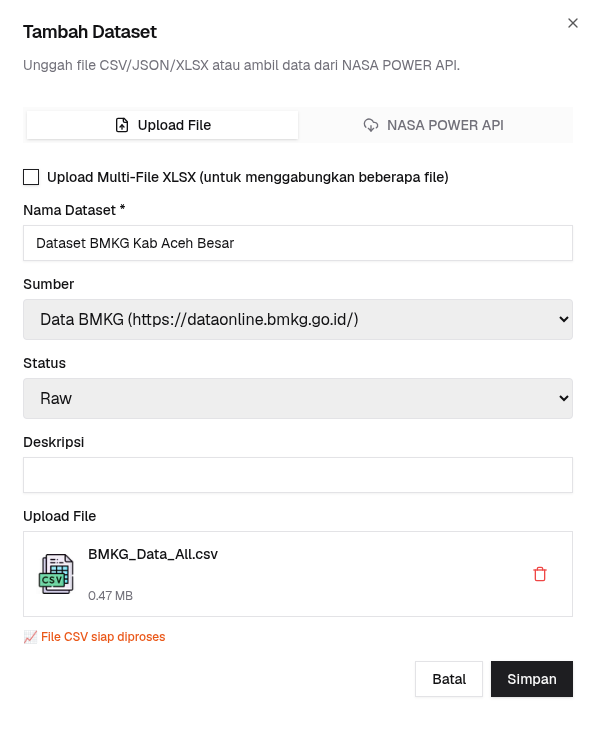
\includegraphics[width=0.4\linewidth]{image/bab4/tambah_dataset_upload.png}
            \caption{Tambah \textit{Dataset} melalui \textit{Upload}}
            \label{fig:tambah_dataset_upload}
        \end{figure}
        \begin{figure}[H]
            \centering
            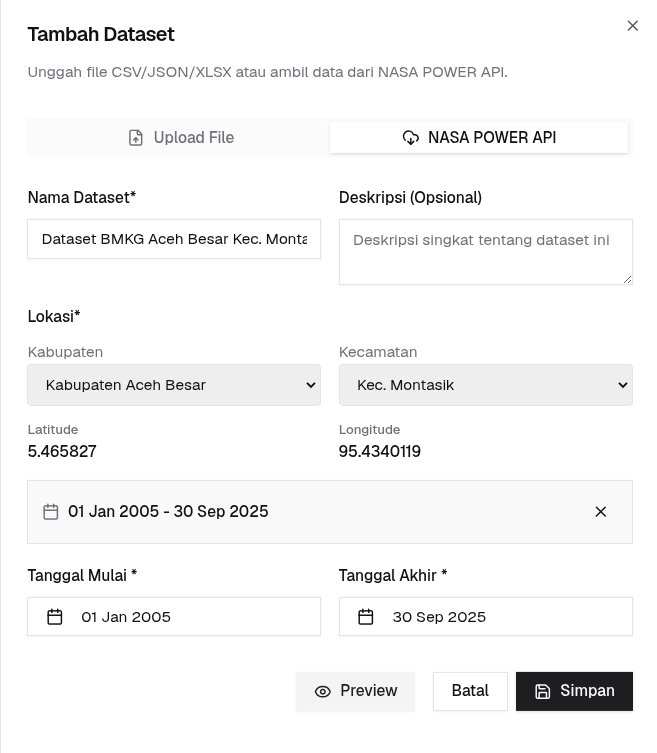
\includegraphics[width=0.4\linewidth]{image/bab4/tambah_dataset_fetch.png}
            \caption{Tambah \textit{Dataset} melalui \textit{Fetch}}
            \label{fig:tambah_dataset_fetch}
        \end{figure}
        Berdasarkan Gambar \ref{fig:tambah_dataset_upload} dan \ref{fig:tambah_dataset_fetch}, terdapat dua mekanisme penambahan data ke dalam sistem. Data BMKG tidak menyediakan \textit{API}, sehingga admin perlu melakukan \textit{upload} manual setelah mengunduh dari portal \textit{online} BMKG. Sebaliknya, NASA POWER menyediakan \textit{public API} yang memungkinkan sistem menarik data secara otomatis melalui \textit{endpoint}. Kedua metode tersebut disimpan ke dalam MongoDB dengan struktur telah diseragamkan.
    \item \textbf{Halaman Detail \textit{dataset}}: Halaman untuk melihat tabel \textit{dataset} yang sudah di \textit{upload}.
        \begin{figure}[H]
            \centering
            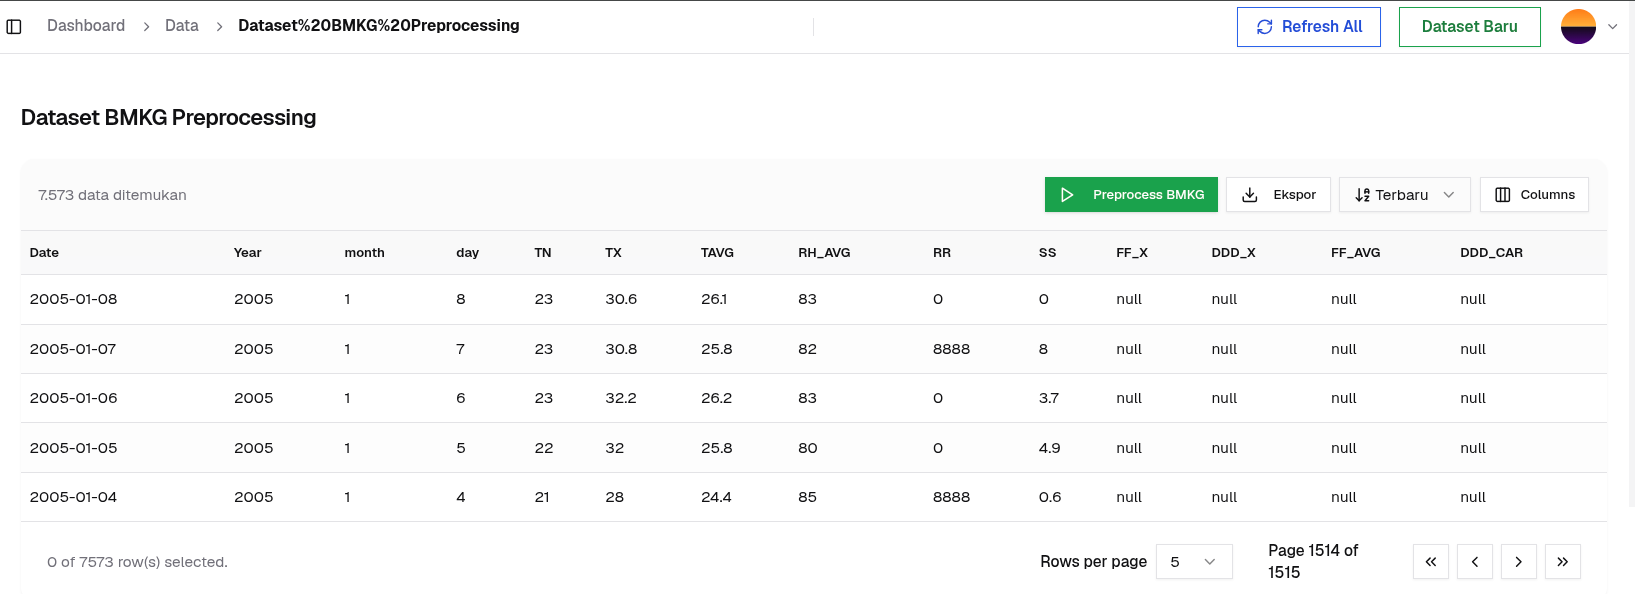
\includegraphics[width=0.95\linewidth]{image/bab4/halaman_detail.png}
            \caption{Halaman Detail \textit{Dataset}}
            \label{fig:halaman_detail}
        \end{figure}
        Gambar \ref{fig:halaman_detail} menampilkan halaman detail dari sebuah \textit{dataset}. Pada halaman ini admin dapat melihat \textit{dataset} dalam bentuk tabel. Terdapat \textit{pagination} untuk melakukan sortir, dan juga visualisasi \textit{time-series}. Pada visualisasi terdapat label data invalid jika ditemukan value dari suatu \textit{column} dari range waktu tertentu, sehingga memudahkan admin dalam mengidentifikasi data yang bermasalah, seperti yang ditunjukkan pada gambar \ref{fig:visualisasi_timeseries} di bawah.
        \begin{figure}[H]
            \centering
            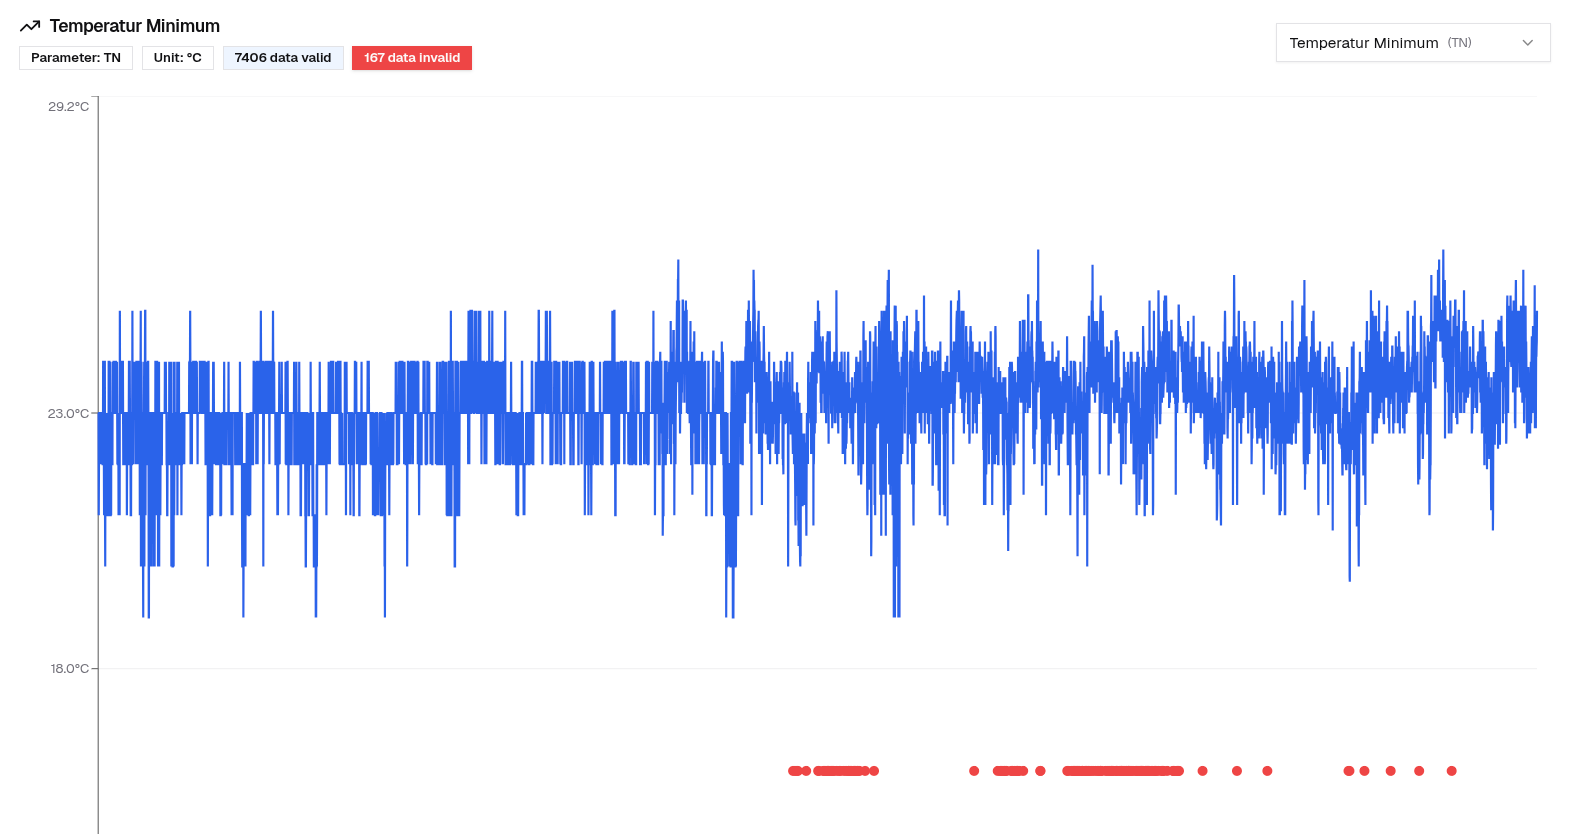
\includegraphics[width=0.95\linewidth]{image/bab4/visualisasi_timeseries.png}
            \caption{Visualisasi \textit{Time-Series}}
            \label{fig:visualisasi_timeseries}
        \end{figure}
        Gambar \ref{fig:visualisasi_timeseries} menyajikan metode penyajian data secara grafis untuk menampilkan perubahan, tren, pola, atau fluktuasi satu atau lebih variabel berdasarkan urutan waktu kronologis. Adapun contoh pada gambar ini adalah menampilkan variabel Temperatur Minimum dari tahun 2005 hingga 2025. Diketahui pada variabel tersebut memiliki sebanyak 7406 data valid dan 167 data invalid.

    \item \textbf{\textit{Preprocessing}}: Admin dapat melakukan \textit{preprocessing} langsung dari halaman detail.
        \begin{figure}[H]
            \centering
            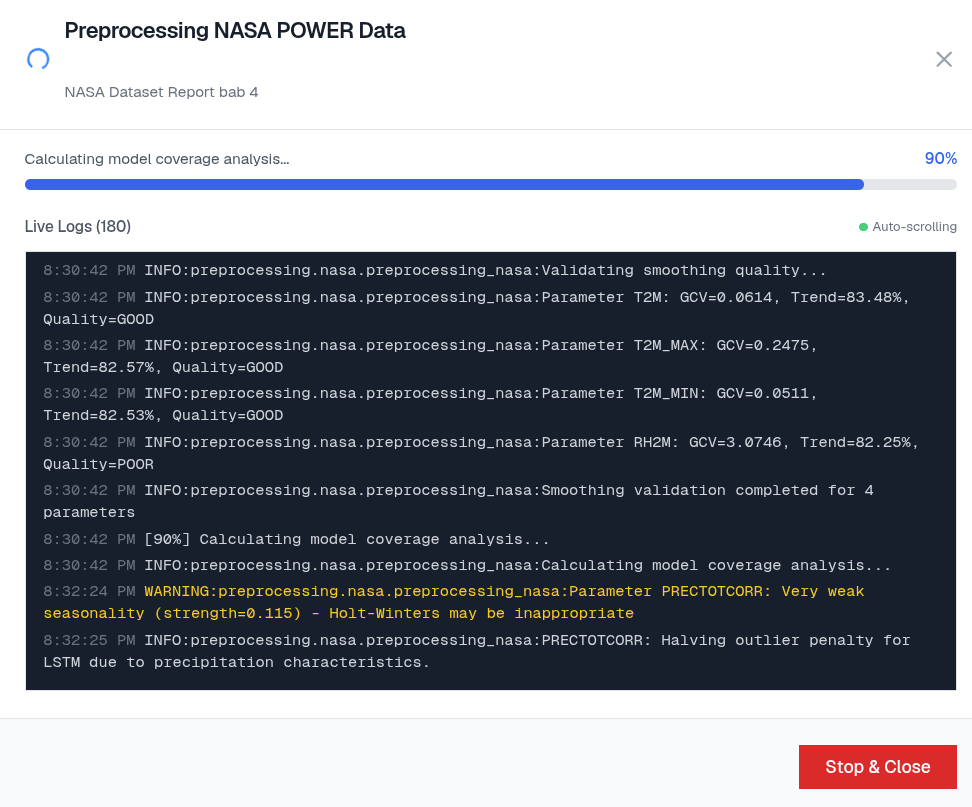
\includegraphics[width=0.6\linewidth]{image/bab4/modal_preprocessing.png}
            \caption{Modal \textit{Preprocessing}}
            \label{fig:modal_preprocessing}
        \end{figure}
        Gambar \ref{fig:modal_preprocessing} menunjukkan fitur \textit{modal preprocessing} pada halaman detail yang digunakan admin untuk menjalankan proses pembersihan \textit{dataset}. Modal ini menampilkan proses yang berjalan pada \textit{backend} Flask secara \textit{real-time}, sehingga admin dapat memantau tahapan dan status eksekusi data secara langsung.
    \item \textbf{Halaman \textit{reports}}: \textit{Summary} hasil \textit{preprocessing}.
        \begin{figure}[H]
            \centering
            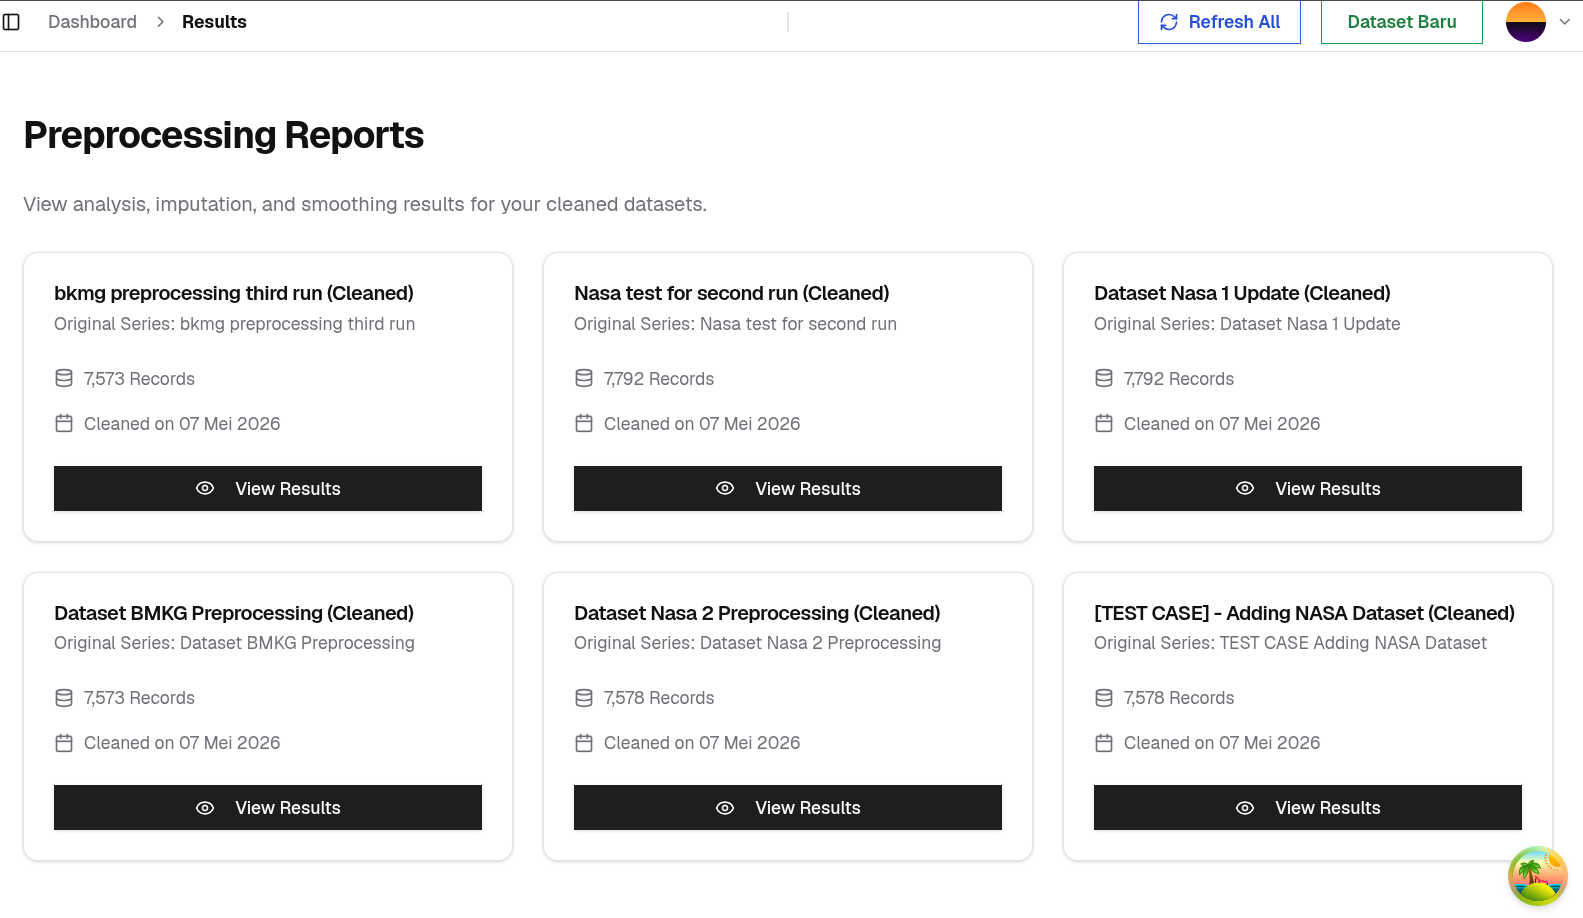
\includegraphics[width=0.95\linewidth]{image/bab4/halaman_reports.png}
            \caption{Halaman \textit{Reports}}
            \label{fig:halaman_reports}
        \end{figure}
        Gambar \ref{fig:halaman_reports} menampilkan halaman \textit{reports} yang berisi ringkasan hasil \textit{preprocessing} data. Admin dapat membuka salah satu hasil pembersihan \textit{dataset}, lalu dilanjutkan ke halaman detail \textit{reports} seperti ditunjukkan pada gambar \ref{fig:halaman_reports_method} sesuai dari tanggal disimpannya.
    \item \textbf{Halaman detail \textit{reports}}: Detail hasil \textit{preprocessing} masing-masing \textit{dataset}.
        \begin{figure}[H]
            \centering
            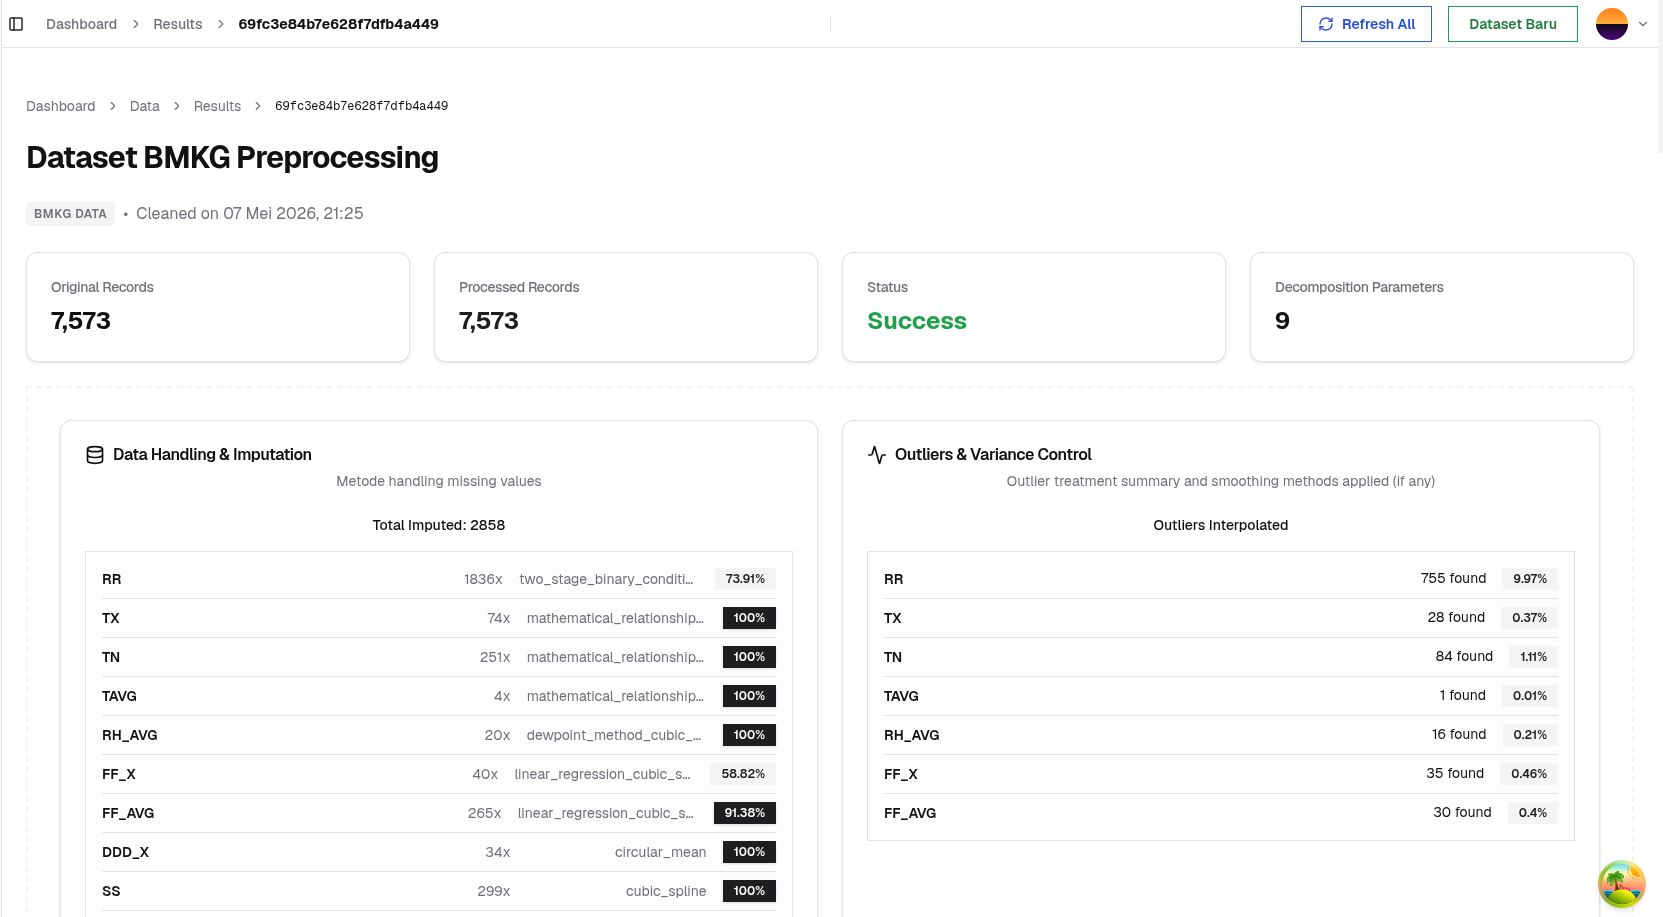
\includegraphics[width=0.95\linewidth]{image/bab4/halaman_reports_method.png}
            \caption{Halaman Detail \textit{Reports}}
            \label{fig:halaman_reports_method}
        \end{figure}
        Setelah \textit{dataset} dibersihkan, disimpan juga \textit{summary} berupa metode yang dilakukan selama proses tersebut berlangsung. Terdapat juga evaluasi GCV dan \textit{Model Coverage} untuk Holt-Winters dan LSTM, sehingga setelah \textit{dataset} bersih, langsung bisa dilakukan pemodelan oleh anggota tim lain.
        \begin{figure}[H]
            \centering
            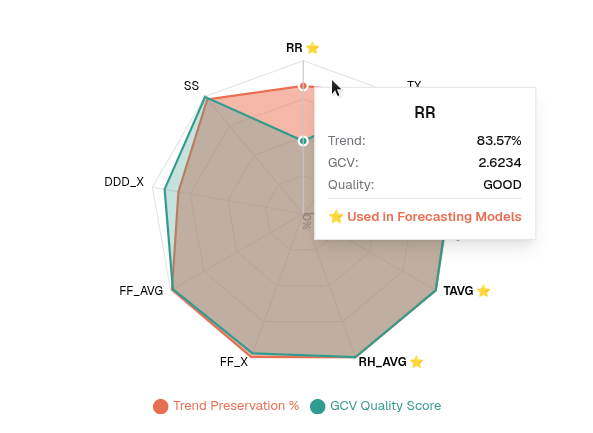
\includegraphics[width=0.5\linewidth]{image/bab4/halaman_reports_gcv.png}
            \caption{GCV \textit{Evaluation}}
            \label{fig:halaman_reports_gcv}
        \end{figure}
        Gambar \ref{fig:halaman_reports_gcv} menampilkan \textit{spider chart} yang model dua metrik kualitas hasil \textit{preprocessing} untuk setiap parameter iklim. Metrik \textit{Trend Preservation} (warna merah) menunjukkan persentase kemiripan arah tren antara data asli dan data hasil \textit{smoothing}, sementara \textit{GCV Quality Score} (warna biru) merepresentasikan nilai GCV yang telah dinormalisasi (skala 0–100 agar semakin tinggi semakin baik). \textit{Spider chart} ini membantu admin membandingkan kualitas antar parameter, sehingga dapat mengidentifikasi data yang sudah siap digunakan untuk pemodelan.
        \begin{figure}[H]
            \centering
            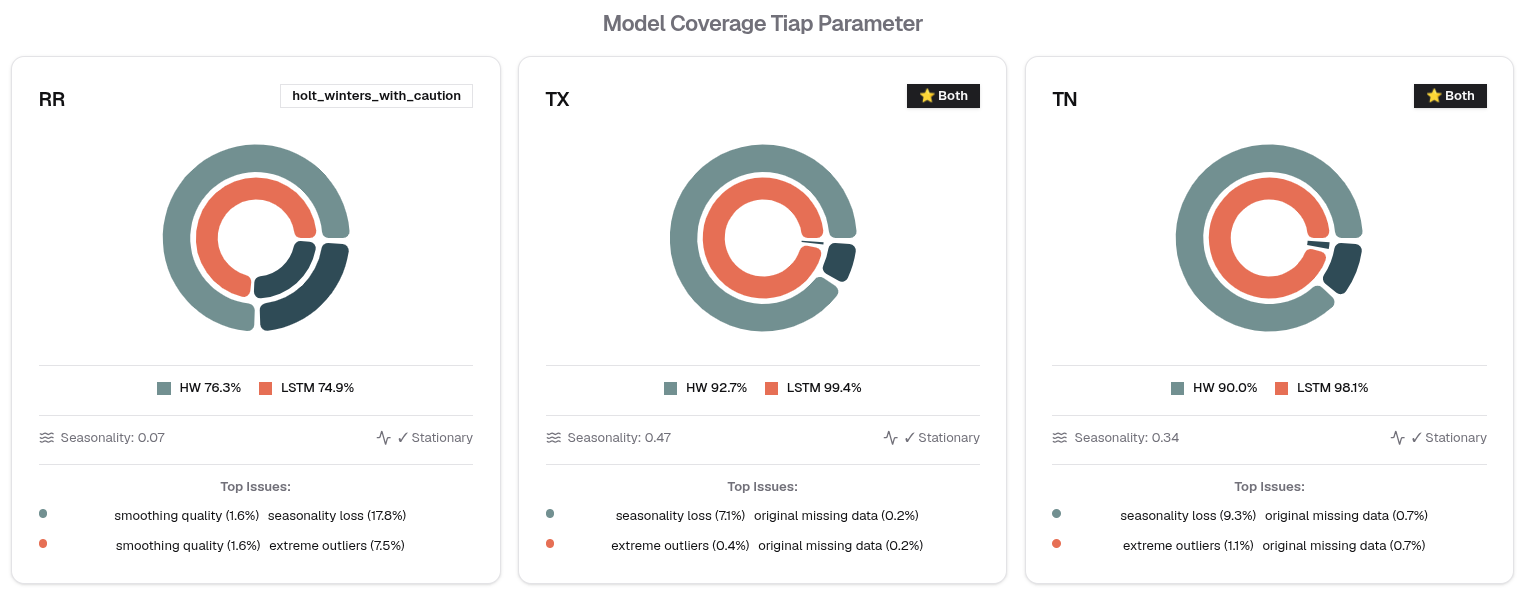
\includegraphics[width=0.95\linewidth]{image/bab4/halaman_reports_coverage.png}
            \caption{\textit{Model Coverage}}
            \label{fig:halaman_reports_coverage}
        \end{figure}
        Gambar \ref{fig:halaman_reports_coverage} menampilkan persentase \textit{model coverage} Holt-Winters dan LSTM sehingga admin mendapatkan rekomendasi model optimal. Berdasarkan nilai \textit{coverage} yang dihitung untuk setiap parameter, sistem memberikan rekomendasi model peramalan yang paling sesuai. Rekomendasi tersebut terdiri atas:
        \begin{itemize}
            \item \textbf{\textit{both}}: kedua model memiliki kualitas data yang sangat baik (coverage >80\% untuk keduanya).
            \item \textbf{\textit{holt\_winters}}: model Holt-Winters yang memiliki coverage sangat baik (>80\%), sementara LSTM di bawahnya.
            \item \textbf{\textit{lstm}}: Model LSTM yang memiliki coverage sangat baik (>80\%).
            \item \textbf{\textit{holt\_winters\_with\_caution}}: coverage Holt-Winters lebih baik (60–80\%) namun belum optimal; model tetap dapat digunakan dengan hati-hati.
            \item \textbf{\textit{lstm\_with\_caution}}: coverage LSTM lebih baik (60–80\%) namun perlu kehati-hatian dalam penggunaannya.
            \item \textbf{\textit{none}}: kedua model memiliki coverage rendah (<60\%), menandakan kualitas data belum memadai untuk peramalan.
        \end{itemize}
        Rekomendasi ini membantu admin dan anggota tim dalam memilih pendekatan pemodelan untuk setiap parameter iklim.
    \item \textbf{Visualisasi dekomposisi}: Dekomposisi variabel iklim setelah \textit{preprocessing}.
        \begin{figure}[H]
            \centering
            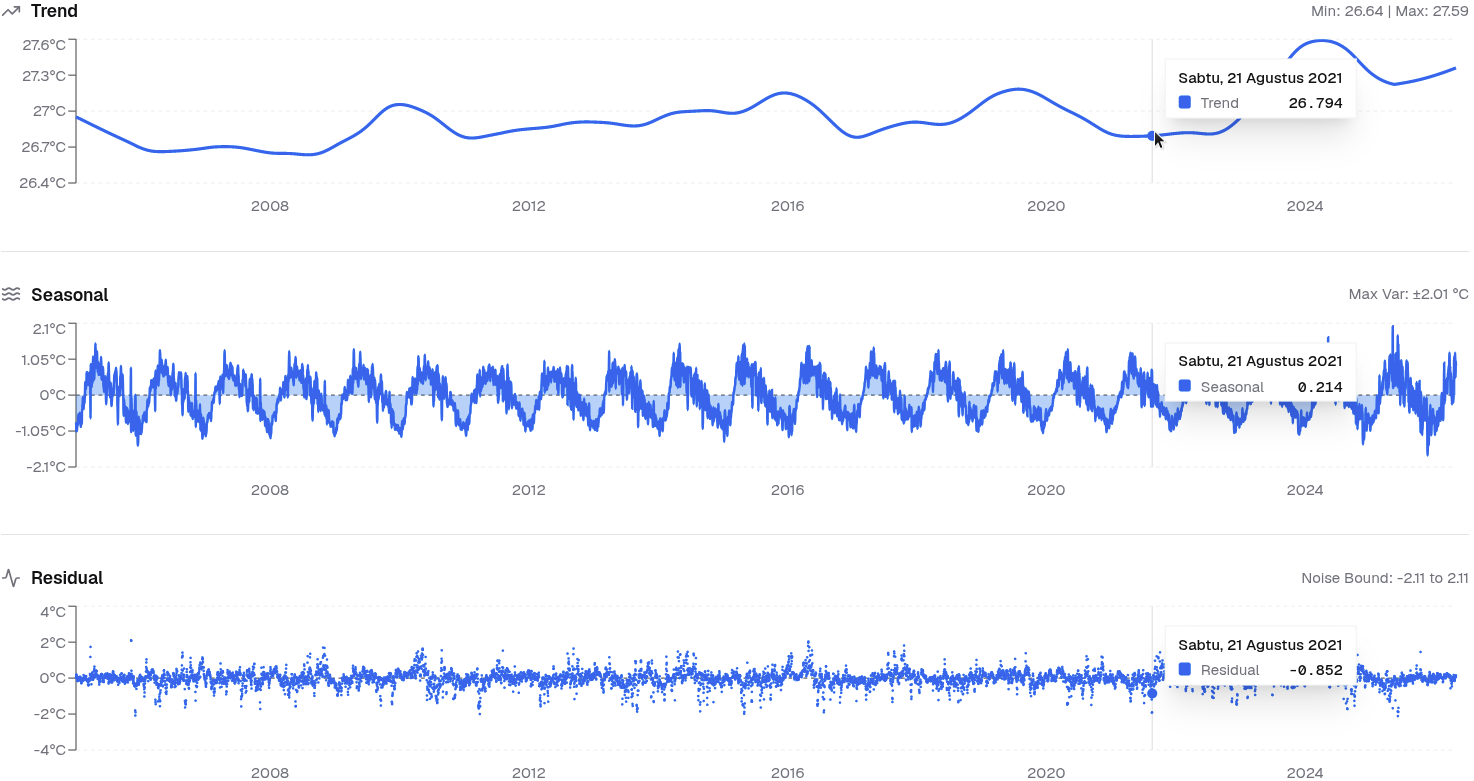
\includegraphics[width=0.95\linewidth]{image/bab4/visualisasi_dekomposisi.png}
            \caption{Visualisasi Dekomposisi}
            \label{fig:visualisasi_dekomposisi}
        \end{figure}
        Gambar \ref{fig:visualisasi_dekomposisi} menampilkan hasil dekomposisi melalui metode (\textit{Seasonal-Trend decomposition using LOESS}) untuk masing-masing variabel iklim. Grafik terbagi menjadi tiga komponen: \textit{Trend} menunjukkan pola data dalam jangka panjang, \textit{Seasonal} menampilkan pola berulang tahunan, dan \textit{Residual} merepresentasikan sisa \textit{noise} setelah tren dan musiman dihilangkan. Admin dapat mengamati bahwa komponen musiman memiliki pola yang stabil dari tahun ke tahun, sedangkan residual umumnya kecil dan acak, menandakan bahwa metode \textit{smoothing} telah berhasil mengekstrak pola utama tanpa menghasilkan \textit{noise} berlebih.
    \item \textbf{Halaman otomasi}: Terdiri dari dua bagian utama, yaitu panel konfigurasi dan riwayat eksekusi.
        \begin{figure}[H]
        \centering
        
\includegraphics[width=0.8\linewidth]{image/bab4/halaman_otomasi.png}
        \caption{Konfigurasi Otomasi}
        \label{fig:halaman_otomasi}
        \end{figure}
        Pada Gambar \ref{fig:halaman_otomasi}, admin dapat mengaktifkan otomasi, memilih frekuensi (mingguan, dua kali seminggu, atau bulanan), waktu eksekusi dan hari pelaksanaan. Admin juga dapat memilih \textit{dataset} mana saja yang akan diproses secara otomatis, baik untuk \textit{refresh} data NASA, maupun \textit{preprocessing} NASA dan BMKG. Setelah konfigurasi disimpan, sistem akan menghitung jadwal berikutnya (ditampilkan pada \textit{Next 5 Scheduled Runs}) dan menjalankan \textit{scheduler} sesuai waktu yang ditentukan. Pada gambar, jadwal frekuensi dua kali seminggu dapat menghasilkan eksekusi pada hari Jumat dan Minggu pukul 11:00. Seluruh proses berjalan di latar belakang tanpa intervensi manual.
        \begin{figure}[H]
        \centering
        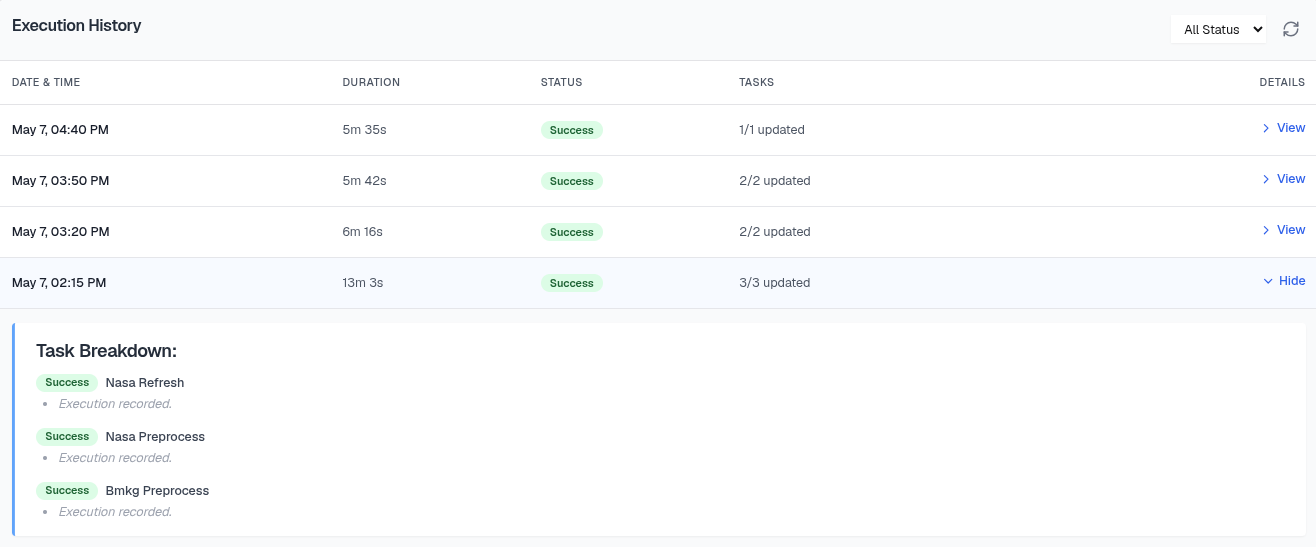
\includegraphics[width=0.95\linewidth]{image/bab4/halaman_otomasi_history.png}
        \caption{Riwayat Eksekusi}
        \label{fig:halaman_otomasi_history}
        \end{figure}
        Gambar \ref{fig:halaman_otomasi_history} menampilkan riwayat eksekusi, mencakup waktu, durasi, status (berhasil/gagal), jumlah \textit{task} yang diperbarui melalui rincian \textit{task breakdown}. Admin dapat memantau apakah otomasi berjalan sesuai jadwal dan mendeteksi jika terjadi kegagalan.
\end{enumerate}

\subsection{Implementasi \textit{backend}}
Implementasi \textit{backend} terdiri atas Next.js untuk autentikasi dan manajemen \textit{dataset}, serta Flask untuk pemrosesan data iklim dan otomasi. Struktur basis data NoSQL yang diimplementasikan pada sistem ditunjukkan pada Gambar \ref{fig:nosql_db_design}.
\begin{figure}[p]
    \centering
    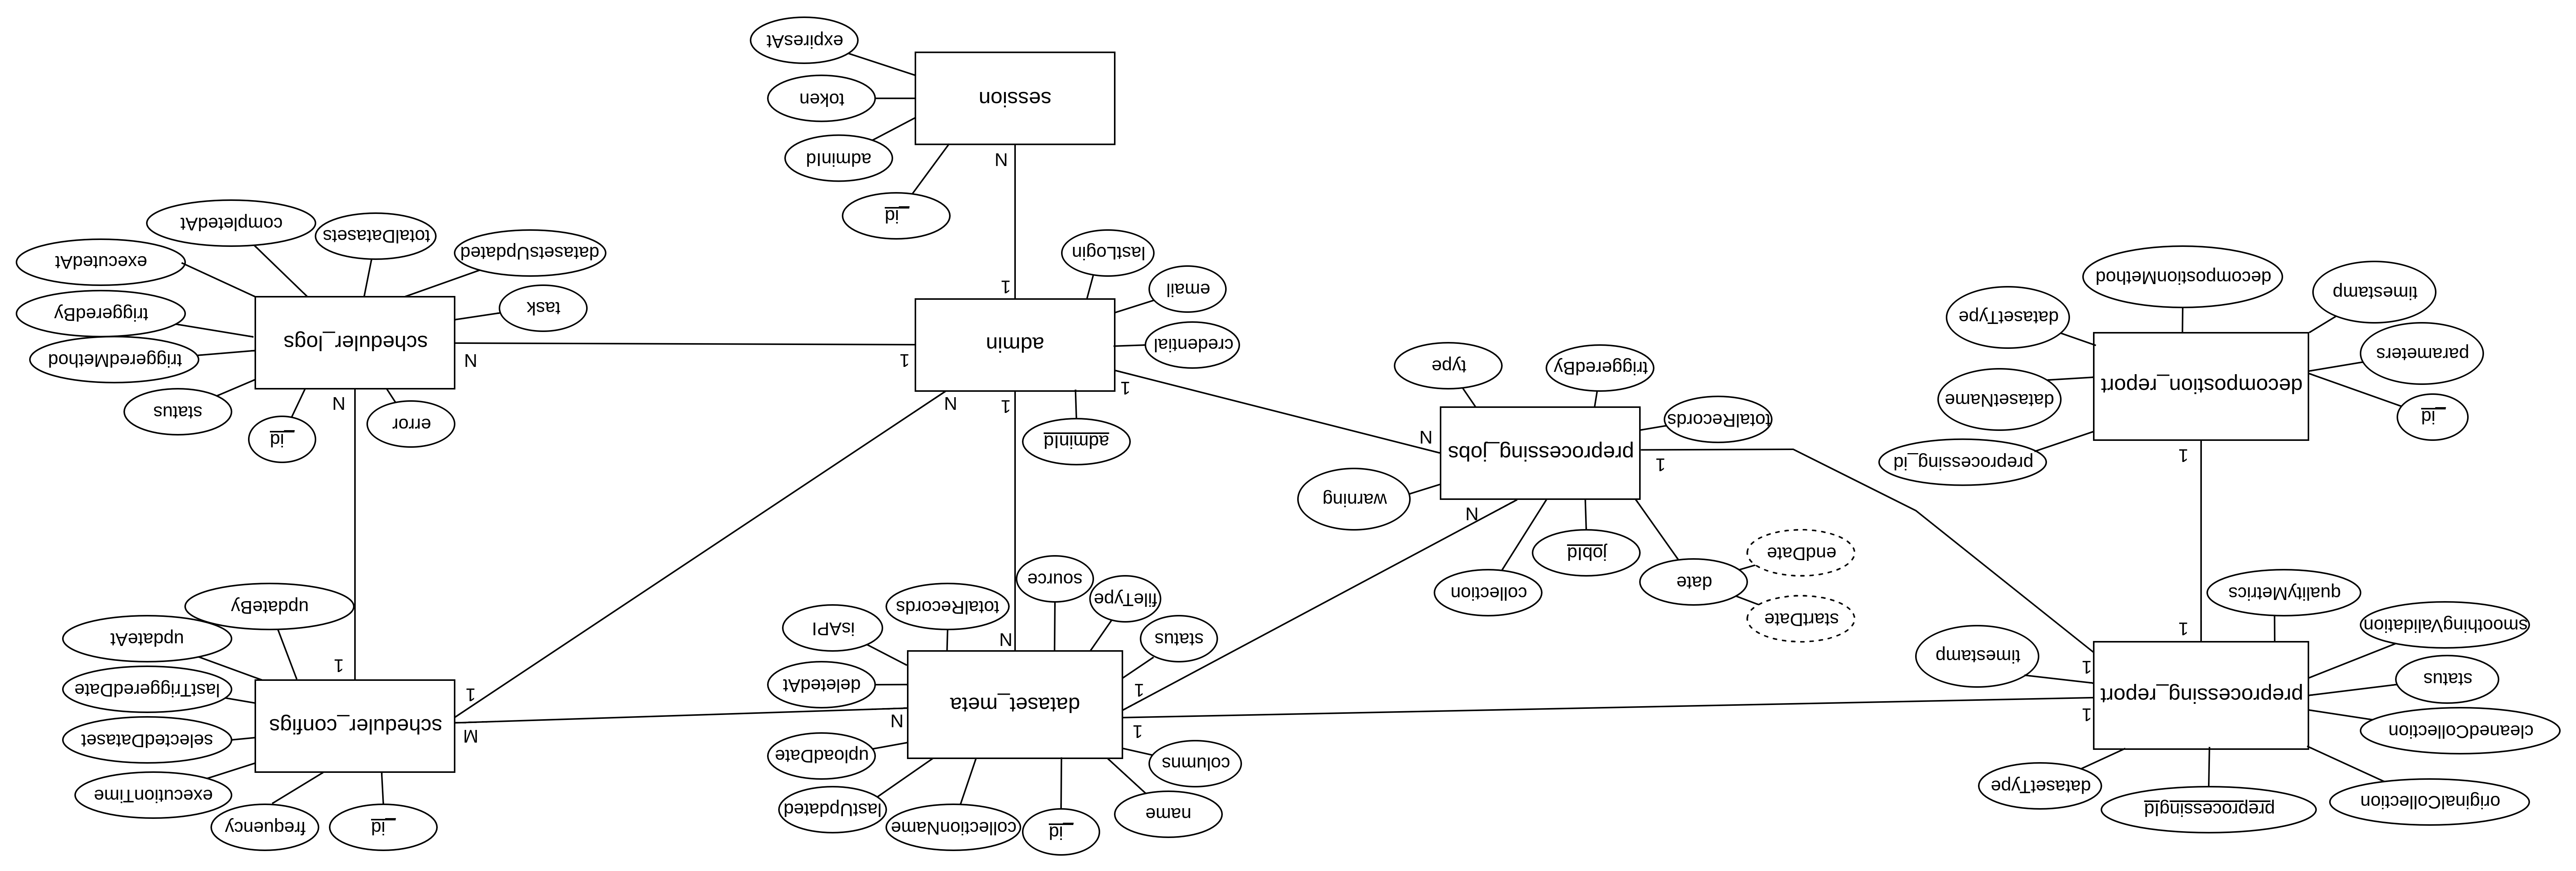
\includegraphics[angle=90,height=0.9\textheight,keepaspectratio]{image/bab4/nosql_db_design.png}
    \caption{\textit{NoSQL Database Design}}
    \label{fig:nosql_db_design}
\end{figure}
\clearpage
\noindent Gambar \ref{fig:nosql_db_design} menunjukkan struktur \textit{NoSQL Database Design} yang menggambarkan hubungan antar \textit{collection} pada MongoDB. Setiap \textit{collection} menyimpan \textit{document} sesuai fungsinya, seperti \textit{admin} untuk data pengguna, \textit{sessions} untuk sesi autentikasi, \textit{dataset\_meta} untuk metadata \textit{dataset}, \textit{preprocessing\_jobs} untuk proses \textit{preprocessing}, \textit{preprocessing\_report} untuk laporan hasil \textit{preprocessing}, \textit{decomposition\_report} untuk hasil dekomposisi, \textit{scheduler\_configs} untuk konfigurasi otomasi, serta \textit{scheduler\_logs} untuk riwayat eksekusi sistem.
\noindent Jika Gambar di atas menekankan hubungan antar \textit{collection} secara konseptual, maka Gambar \ref{fig:document_schema_diagram} memperjelas struktur internal setiap \textit{collection}, meliputi \textit{field}, tipe data, serta \textit{method} yang tersedia. \textit{Diagram} ini juga menunjukkan mekanisme \textit{embedding} dan \textit{referencing} antar \textit{document}, yaitu penyimpanan data secara textit{embedded} di dalam satu \textit{document}, maupun penyimpanan data secara terpisah yang dihubungkan melalui \textit{field} referensi (\textit{ObjectId} atau \textit{string}) ke \textit{collection} lain.
\begin{figure}[H]
    \centering
    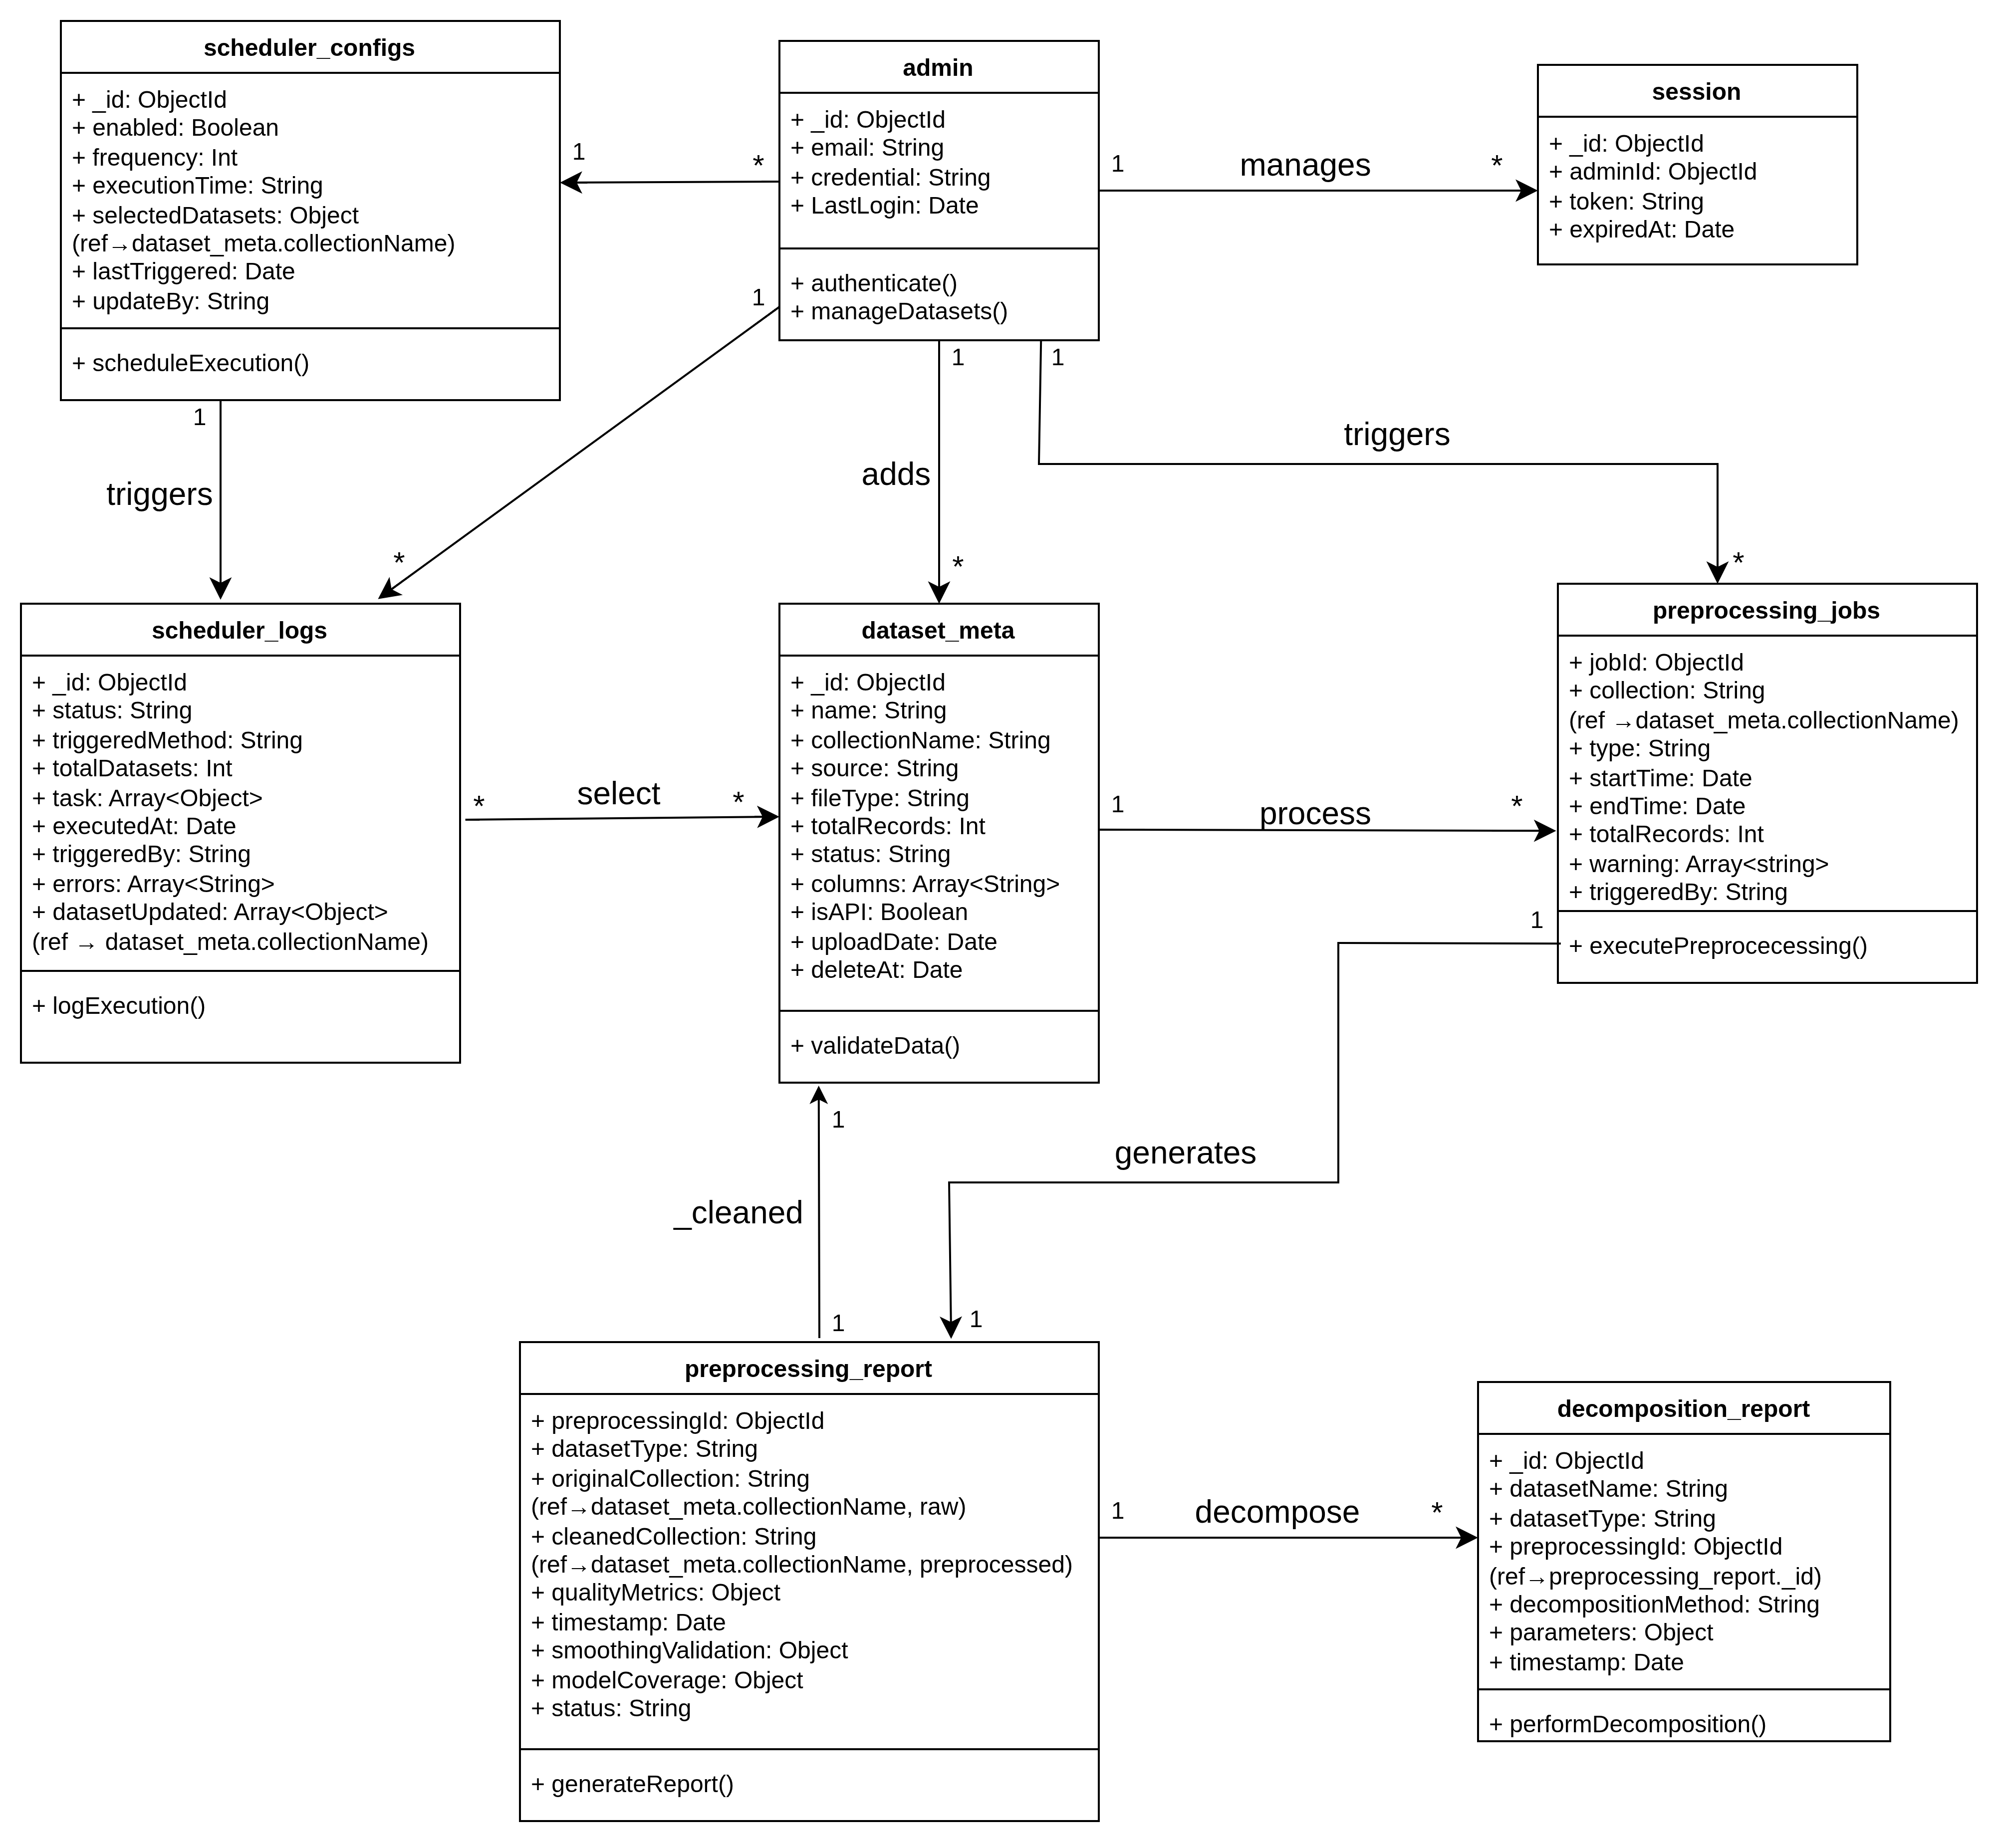
\includegraphics[width=0.8\linewidth]{image/bab4/document_schema_diagram.png}
    \caption{\textit{Document Schema Diagram}}
    \label{fig:document_schema_diagram}
\end{figure}
\noindent Gambar \ref{fig:document_schema_diagram} menampilkan struktur \textit{document} pada setiap \textit{collection} beserta mekanisme \textit{embedding} dan \textit{referencing} yang diterapkan, secara spesifik dijabarkan sebagai berikut:
\begin{enumerate}[(a)]
    \item \textbf{Autentikasi}: \textit{collection} \textit{session} menyimpan \textit{field adminId} bertipe \textit{ObjectId} yang menjadi referensi langsung (\textit{hard reference}) ke \textit{collection admin}.

    \item \textbf{Metadata \textit{Dataset}}: \textit{collection dataset\_meta} menyimpan seluruh metadata \textit{dataset} secara mandiri tanpa referensi keluar, sehingga berfungsi sebagai \textit{collection} acuan (\textit{lookup}) bagi \textit{collection} lain melalui \textit{field collectionName}.

    \item \textbf{\textit{Preprocessing}}: \textit{collection preprocessing\_jobs} menyimpan \textit{field collection} bertipe \textit{String} yang mereferensikan \textit{dataset\_meta.collectionName} (\textit{soft reference}). \textit{Collection preprocessing\_report} menyimpan dua \textit{soft reference} sekaligus, yaitu \textit{originalCollection} yang merujuk pada \textit{dataset} mentah dan \textit{cleanedCollection} yang merujuk pada \textit{dataset} hasil \textit{preprocessing}, sementara data pendukung seperti \textit{qualityMetrics}, \textit{smoothingValidation}, dan \textit{modelCoverage} disimpan secara \textit{embedded} di dalam \textit{document} yang sama.

    \item \textbf{Dekomposisi}: \textit{collection decomposition\_report} menyimpan \textit{field preprocessingId} bertipe \textit{ObjectId} sebagai referensi langsung ke \textit{preprocessing\_report.\_id}, sedangkan hasil dekomposisi setiap parameter disimpan secara \textit{embedded} pada \textit{field parameters}.

    \item \textbf{Penjadwalan}: \textit{collection scheduler\_configs} menyimpan \textit{field selectedDatasets} berupa \textit{object embedded} yang isinya merupakan kumpulan \textit{soft reference} ke \textit{dataset\_meta.collectionName}, sehingga merepresentasikan relasi \textit{many-to-many} tanpa \textit{foreign key} formal. Pola serupa juga diterapkan pada \textit{collection scheduler\_logs} melalui \textit{field datasetUpdated}.
\end{enumerate}

\noindent Perbedaan mekanisme \textit{embedding} dan \textit{referencing} tersebut menunjukkan bahwa desain basis data pada sistem ini mengutamakan performa \textit{query} dengan meminimalkan proses \textit{join} antar \textit{collection}, sekaligus tetap menjaga keterhubungan data melalui \textit{referencing} pada bagian yang membutuhkan penelusuran \textit{traceability} antar \textit{document}.


\begin{enumerate}
    \item \textbf{Fitur Tambah \textit{Dataset} dan Penyimpanan Metadata}: \textit{Admin} dapat menambahkan \textit{dataset} BMKG dan NASA POWER menggunakan 2 metode berikut:
    \begin{figure}[H]
        \centering
        \begin{minipage}{0.45\linewidth}
            \centering
            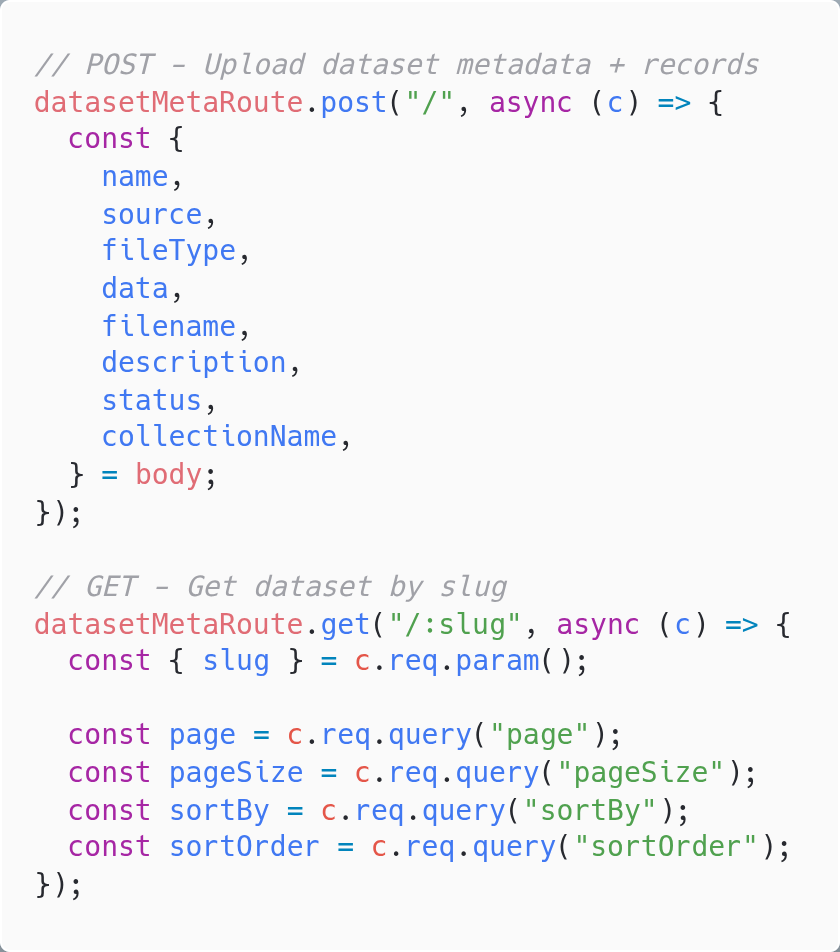
\includegraphics[width=\linewidth]{image/bab4/endpoint_datasetMeta.png}
            \label{fig:endpoint_meta}
        \end{minipage}
        \hspace{0.05\linewidth}
        \begin{minipage}{0.45\linewidth}
            \centering
            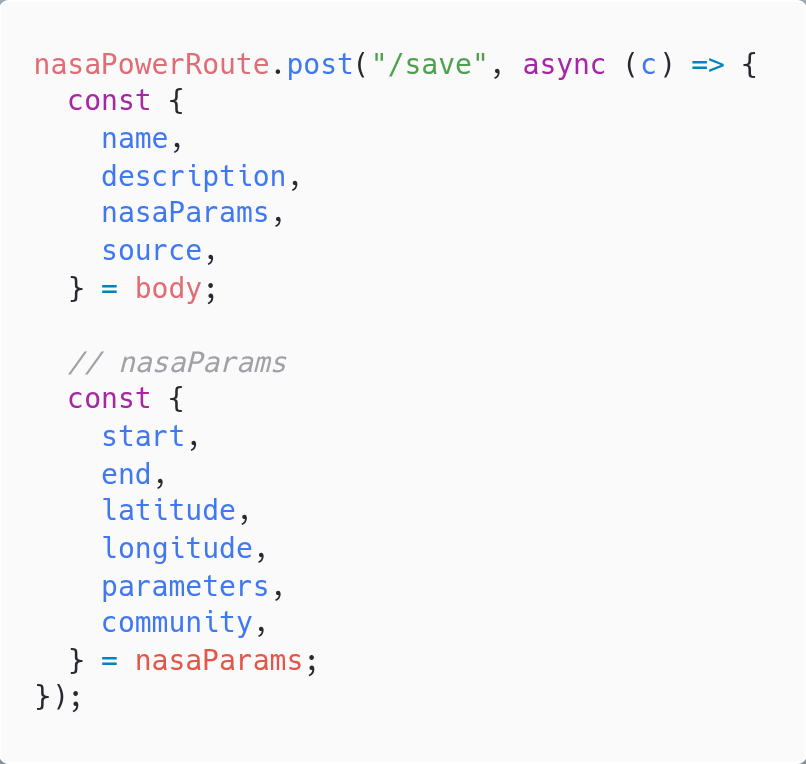
\includegraphics[width=\linewidth]{image/bab4/endpoint_nasa.png}
            \label{fig:endpoint_nasa}
        \end{minipage}
        \caption{Potongan kode \textit{endpoint} \textit{Dataset} BMKG dan NASA POWER}
        \label{fig:endpoint_bmkg_nasa}
    \end{figure}
        Gambar \ref{fig:endpoint_bmkg_nasa} memperlihatkan implementasi \textit{endpoint} untuk mengupload \textit{dataset}. File csv yang diunggah akan di-\textit{parse} pada sisi \textit{frontend}. \textit{Backend} menyimpan ke dalam \textit{collection} baru disertai informasi \textit{metadata} agar informasi \textit{dataset} dapat dikelola. Gambar kedua memiliki metode POST yang sama, tetapi \textit{dataset} akan di GET terlebih dahulu dari sumber menggunakan parameter nasaParams.

    \item \textbf{Fitur Jalankan \textit{Preprocessing}}: Fitur ini memungkinkan admin menjalankan \textit{preprocessing} melalui \textit{trigger button}.
        \begin{figure}[H]
            \centering
            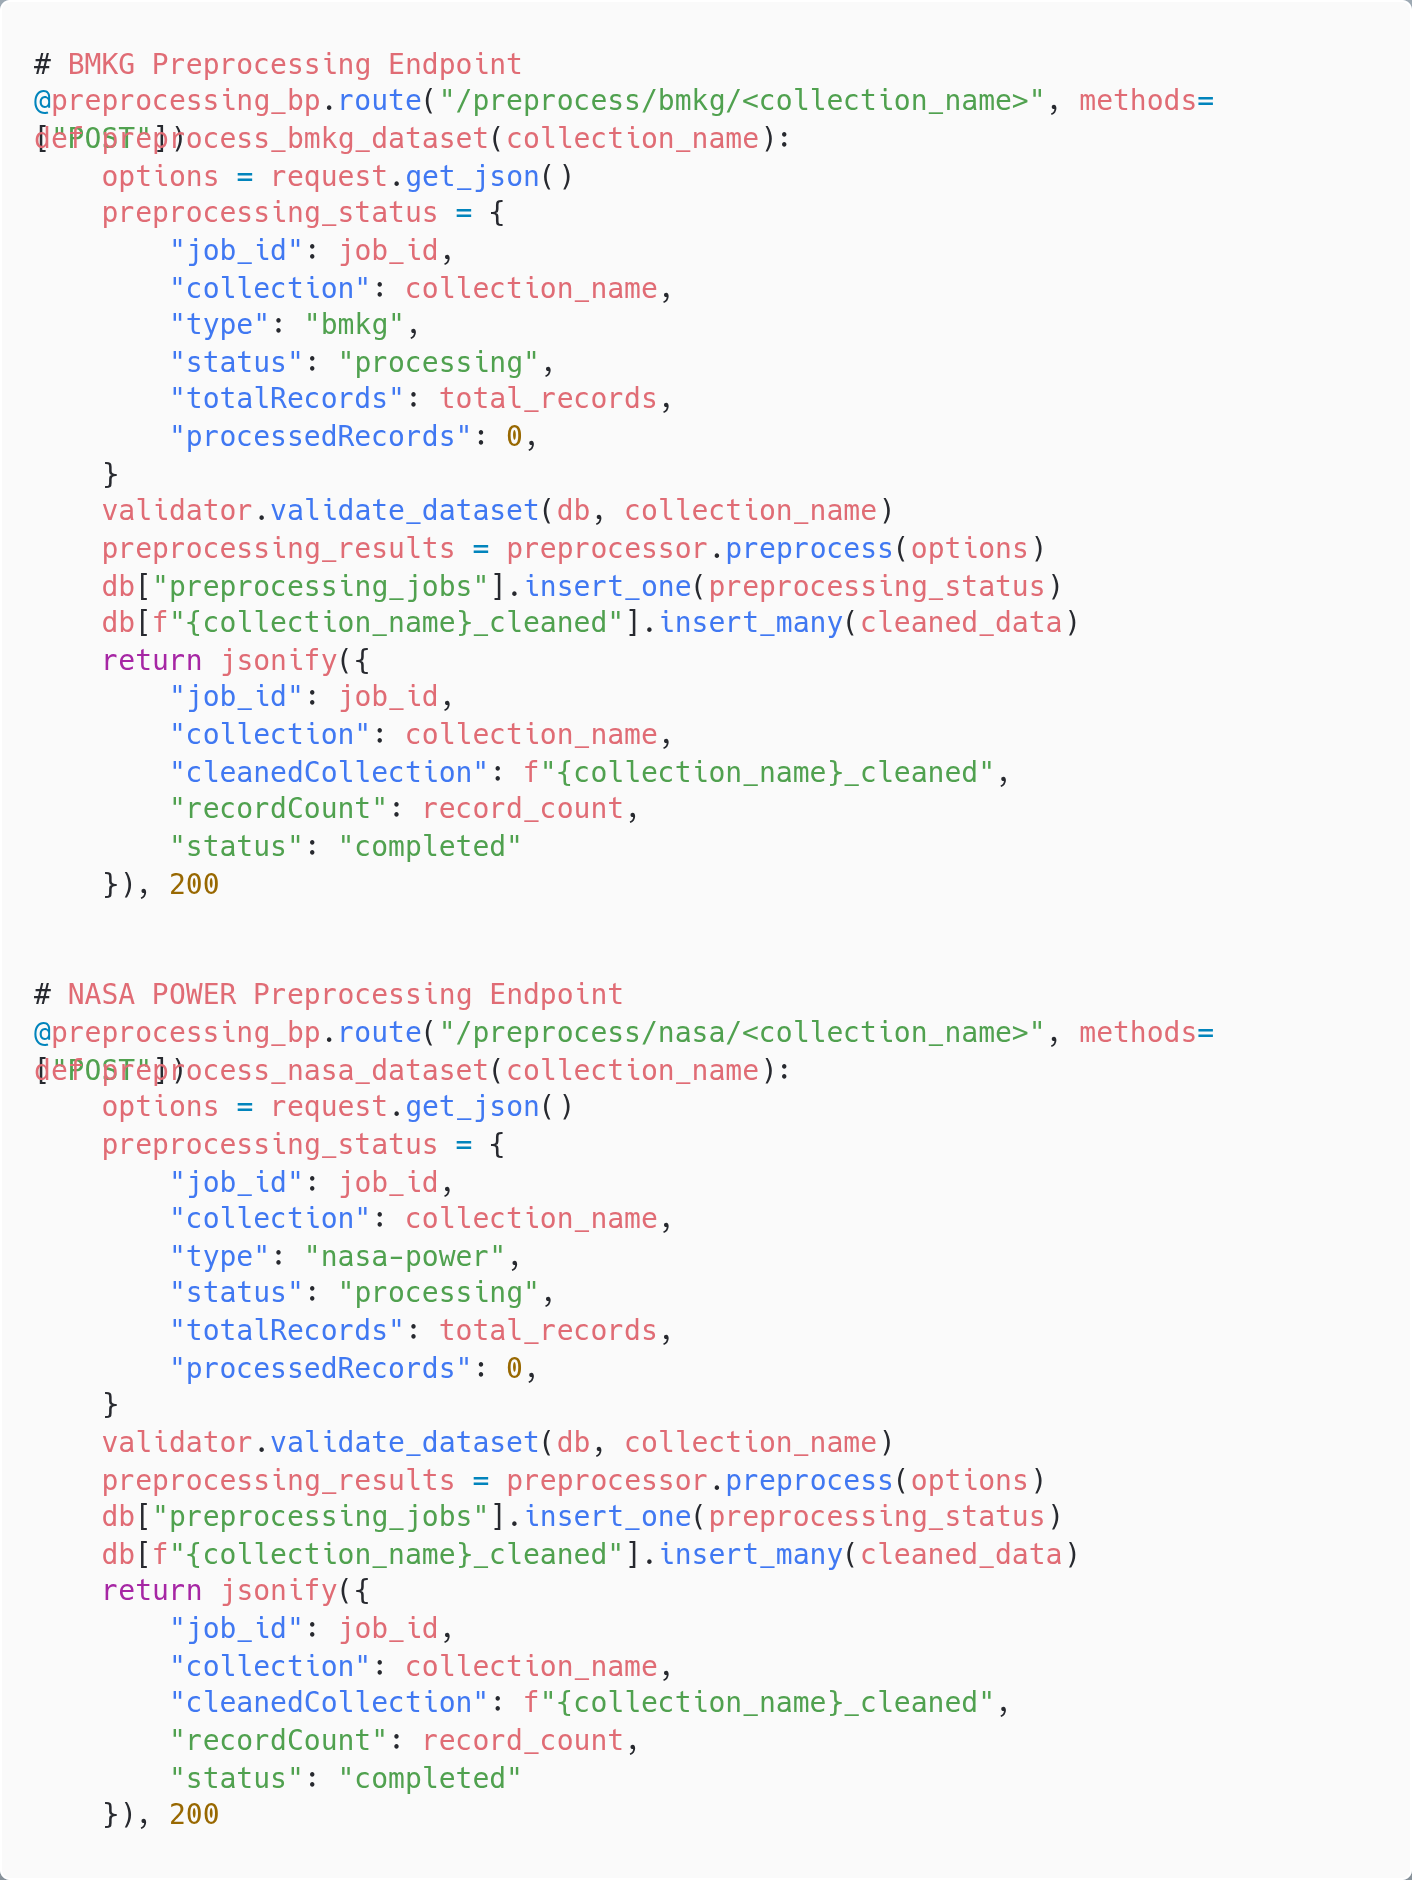
\includegraphics[width=0.4\linewidth]{image/bab4/endpoint_preprocessing.png}
            \caption{Potongan kode \textit{endpoint Preprocessing}}
            \label{fig:endpoint_preprocessing}
        \end{figure}
        Gambar \ref{fig:endpoint_preprocessing} menampilkan implementasi \textit{endpoint} \textit{preprocessing} untuk \textit{dataset} BMKG dan NASA POWER menggunakan \textit{framework} Flask. \textit{Endpoint} menerima parameter \textit{collection\_name} untuk menentukan \textit{dataset} yang akan diproses dari MongoDB. Sistem kemudian melakukan validasi, menjalankan proses \textit{preprocessing}, serta menyimpan hasil bersih ke \textit{collection} baru dengan akhiran \textit{\_cleaned}.  Ketika proses berlangsung, sistem mencatat status ke dalam \textit{collection preprocessing\_jobs} agar proses dapat dipantau. \textit{Endpoint} juga menjalankan fungsi \textit{executePreprocessing()} yang menghasilkan \textit{preprocessing report} berisi \textit{summary} hasil pembersihan data. Setelah proses selesai, status diperbarui menjadi \textit{preprocessed} sehingga \textit{dataset} siap digunakan untuk pemodelan.
    
    \item \textbf{Fitur \textit{Reports}}: Yaitu hasil \textit{preprocessing} yang disimpan ke dalam \textit{collection} \textit{preprocessing\_report}.
        \begin{figure}[H]
            \centering
            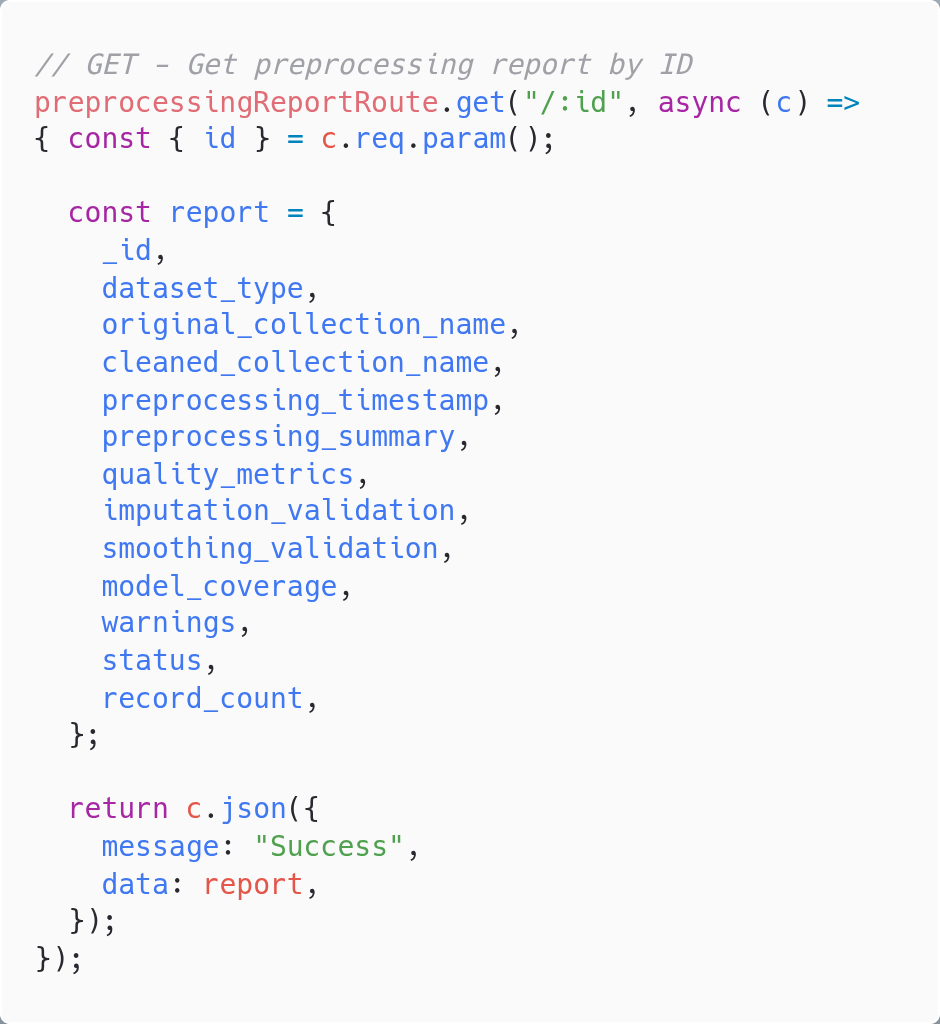
\includegraphics[width=0.4\linewidth]{image/bab4/endpoint_report.png}
            \caption{Potongan kode \textit{endpoint Report}}
            \label{fig:endpoint_report}
        \end{figure}
    Gambar \ref{fig:endpoint_report} menampilkan implementasi \textit{endpoint} untuk mengambil \textit{preprocessing report} berdasarkan \textit{id}. Laporan ini disimpan ke dalam \textit{collection preprocessing\_report} setelah proses \textit{preprocessing} selesai. Informasi yang disimpan meliputi jenis \textit{dataset}, nama \textit{collection} asli dan hasil pembersihan, \textit{summary preprocessing}, metrik kualitas data, validasi imputasi atau \textit{smoothing}, cakupan model, jumlah data sebelum dan sesudah diproses, serta status proses.  Laporan \textit{preprocessing} digunakan sebagai acuan pada tahap dekomposisi deret waktu.
    \item \textbf{Fitur Dekomposisi}: Setiap \textit{preprocessing} menghasilkan \textit{preprocessing\_report} dan \textit{decomposition\_report}.
        \begin{figure}[H]
            \centering
            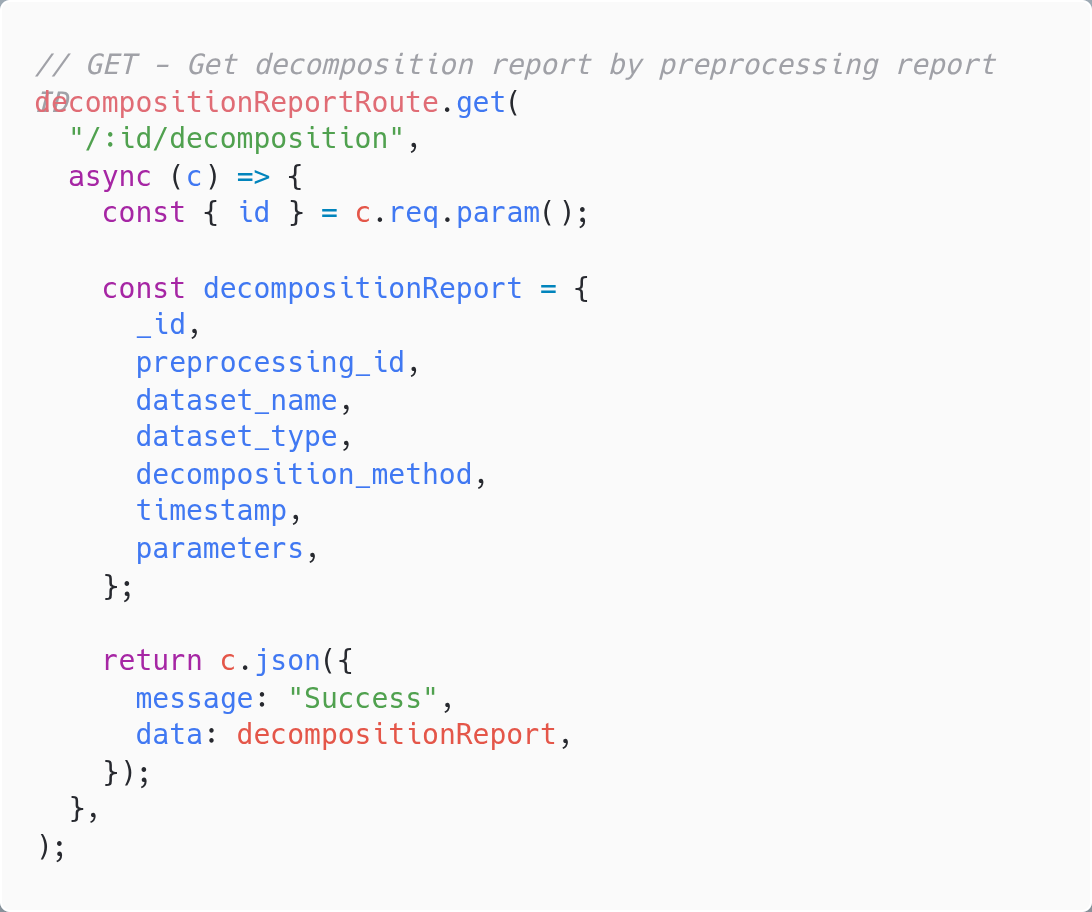
\includegraphics[width=0.4\linewidth]{image/bab4/endpoint_decomposition.png}
            \caption{Potongan kode \textit{endpoint} \textit{Decomposition}}
            \label{fig:endpoint_decomposition}
        \end{figure}
    Gambar \ref{fig:endpoint_decomposition} menjelaskan implementasi \textit{endpoint} untuk mengambil \textit{decomposition report} berdasarkan id \textit{preprocessing\_report}. Setiap proses \textit{preprocessing} menghasilkan \textit{decomposition\_report} yang menyimpan hasil pemisahan komponen data menjadi \textit{trend}, \textit{seasonal}, dan \textit{residual}. Dengan demikian, sistem dapat melacak keterkaitan antara \textit{dataset} mentah, hasil \textit{preprocessing}, dan hasil dekomposisi secara terstruktur.
    \item \textbf{Fitur Penjadwalan}: Admin dapat menjadwalkan \textit{preprocessing} secara otomatis.
    \begin{enumerate}[(a)]
        \item \textbf{Konfigurasi}
        \begin{figure}[H]
            \centering
            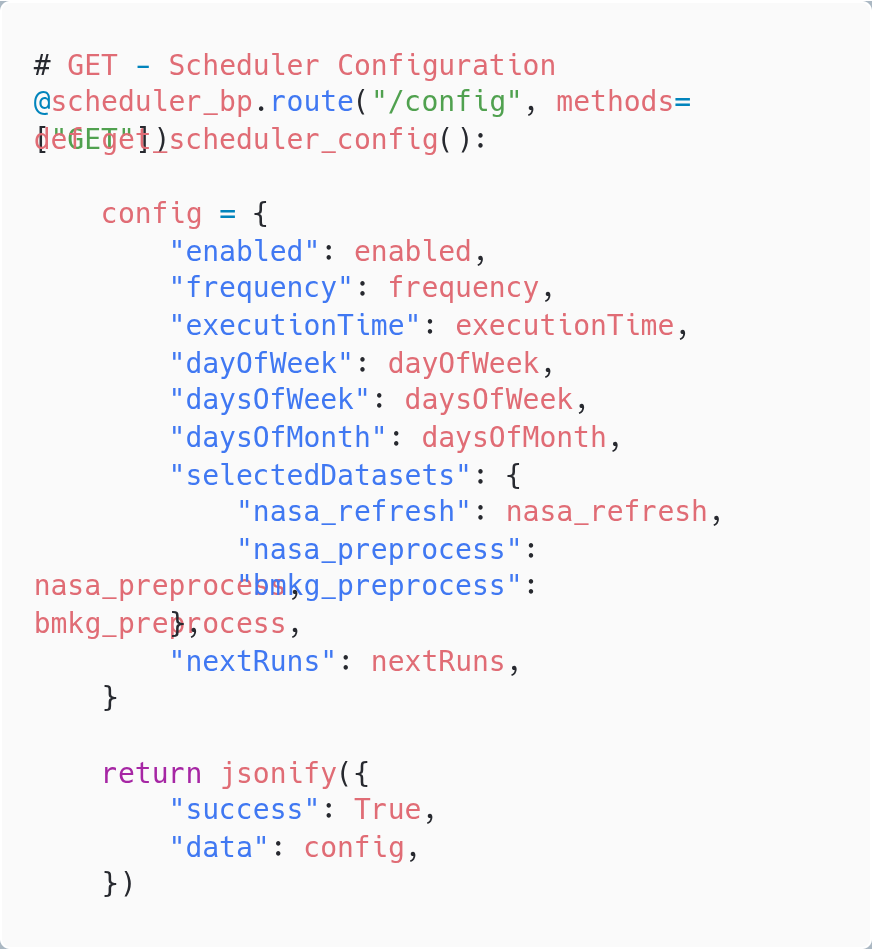
\includegraphics[width=0.4\linewidth]{image/bab4/endpoint_config.png}
            \caption{Potongan kode \textit{endpoint} Konfigurasi}
            \label{fig:endpoint_config}
        \end{figure}
        \item \textbf{\textit{Trigger}}
        \begin{figure}[H]
            \centering
            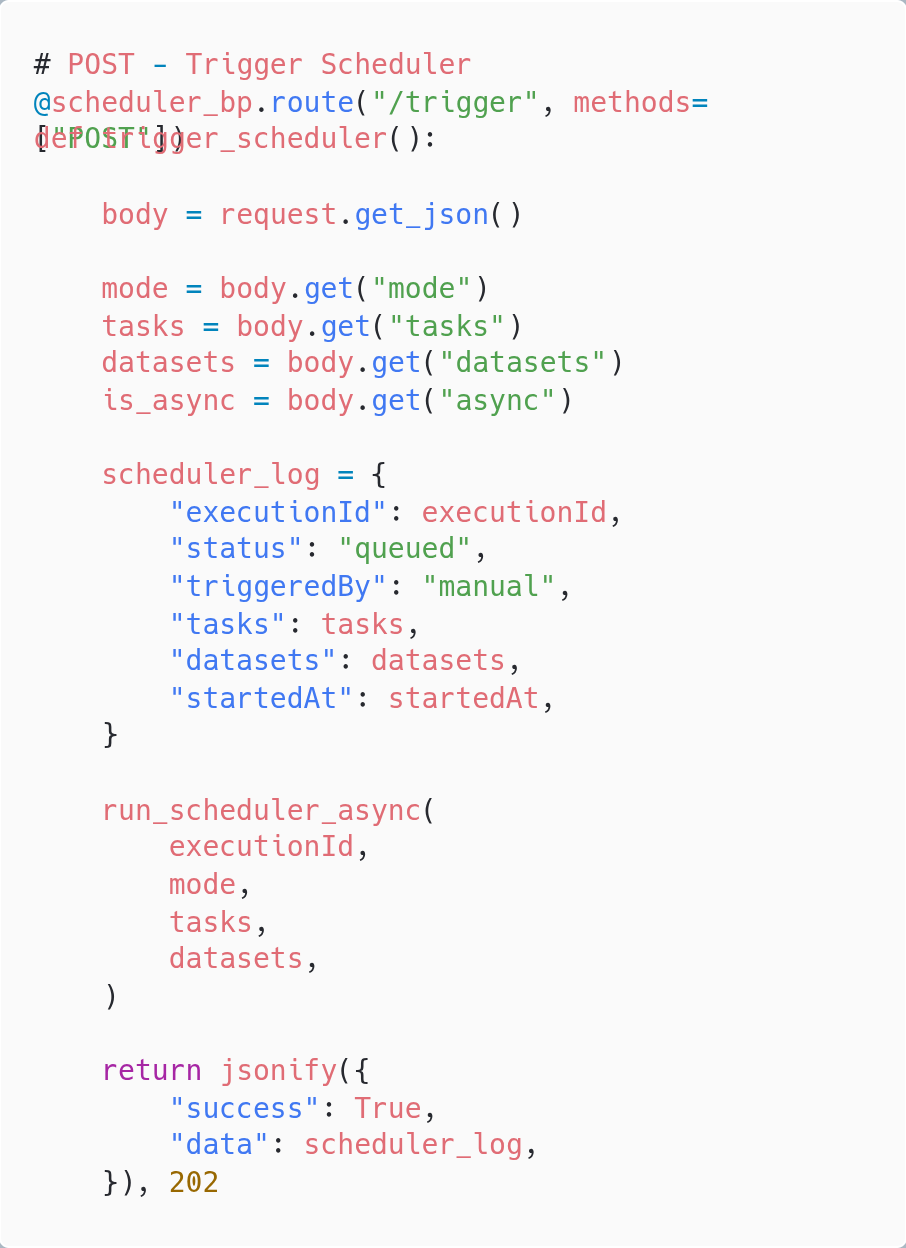
\includegraphics[width=0.4\linewidth]{image/bab4/endpoint_trigger.png}
            \caption{Potongan kode \textit{endpoint} \textit{Trigger}}
            \label{fig:endpoint_trigger}
     \end{figure}
     \end{enumerate}
     Gambar \ref{fig:endpoint_config} menunjukkan \textit{endpoint} konfigurasi penjadwalan yang digunakan untuk mengatur frekuensi eksekusi, waktu berjalan, serta \textit{dataset} yang akan diproses. Konfigurasi tersebut kemudian digunakan oleh sistem otomasi untuk menentukan proses \textit{refresh} \textit{dataset} NASA POWER, dan \textit{preprocessing} BMKG maupun NASA POWER. Selanjutnya, gambar \ref{fig:endpoint_trigger} menampilkan \textit{endpoint} untuk menjalankan \textit{scheduler}. \textit{Endpoint} menjalankan proses otomasi seperti \textit{refresh dataset}, \textit{preprocessing}, serta pencatatan \textit{history} ke dalam \textit{collection} {scheduler\_logs}.  
\end{enumerate}

\subsection{Analisa \textit{dataset}}
    \begin{enumerate}[(a)]
        \item \textbf{Persiapan Data}: \textit{Dataset} menggunakan dua sumber utama, yaitu BMKG yang dapat diunduh dari situs \url{https://dataonline.bmkg.go.id}, dan NASA POWER yang diakses melalui \textit{public API} \url{https://power.larc.nasa.gov/api/temporal/daily/openapi.json}.
        \item \textbf{Observasi Deskriptif}: Observasi deskriptif dilakukan untuk memahami karakteristik awal setiap parameter iklim sebelum dilakukan \textit{preprocessing}. Tujuannya adalah mengidentifikasi kelengkapan data, mendeteksi potensi nilai ekstrem atau data tidak valid, serta menentukan strategi imputasi yang tepat. Adapun rentang pengambilan pada kedua \textit{dataset} tersebut selama 20 tahun, dimulai dari 1 Januari 2005 - 30 September 2025. Berikut disajikan statisik data untuk tiap variabel iklim pada tabel \ref{tab:statistik_bmkg} dan tabel \ref{tab:statistik_nasa}.
        \begin{table}[H] 
            \centering
            \caption{Statistik Data BMKG}
            \label{tab:statistik_bmkg}
            \begin{adjustbox}{max width=\textwidth}
            \small
            \begin{tabular}{|l|c|c|c|c|c|c|c|c|c|}
            \hline
            \textbf{Data} & \textbf{Keterangan} & \textbf{TN} & \textbf{TX} & \textbf{TAVG} & \textbf{RH\_AVG} & \textbf{RR} & \textbf{SS} & \textbf{FF\_X} & \textbf{DDD\_X} \\
            & & \textbf{(°C)} & \textbf{(°C)} & \textbf{(°C)} & \textbf{(\%)} & \textbf{(mm)} & \textbf{(jam)} & \textbf{(m/s)} & \textbf{(°)} \\
            \hline\hline
            \multirow{9}{*}{\textbf{BMKG}} 
            & Jumlah Data & 7565 & 7565 & 7565 & 7565 & 7565 & 7565 & 7565 & 7565 \\
            \cline{2-10}
            & Data \textit{Invalid} & 80 & 56 & 8 & 2 & 2770 & 607 & 300 & 1564 \\
            \cline{2-10}
            & Minimum & 13 & 24.80 & 23.30 & 44 & 0 & 0.10 & 2 & 1 \\
            \cline{2-10}
            & Q1 & 22.10 & 31.80 & 26.50 & 74 & 0 & 3 & 3 & 135 \\
            \cline{2-10}
            & Median & 23 & 32.80 & 27.50 & 81 & 1.80 & 5.10 & 4 & 180 \\
            \cline{2-10}
            & \textit{Mean} & 22.86 & 32.75 & 27.70 & 79.86 & 7.56 & 4.93 & 4.03 & 215.46 \\
            \cline{2-10}
            & Q3 & 23.60 & 34 & 28.90 & 87 & 8.60 & 6.90 & 5 & 315 \\
            \cline{2-10}
            & Maksimum & 28.60 & 37.60 & 32.90 & 100 & 180.80 & 11.50 & 16 & 360 \\
            \cline{2-10}
            & Std. Dev & 1.33 & 1.69 & 1.65 & 9.41 & 14.02 & 2.54 & 1.35 & 92.27 \\
            \hline
            \end{tabular}
            \end{adjustbox}
        \end{table}
        \begin{table}[H] 
            \centering
            \caption{Statistik Data NASA POWER}
            \label{tab:statistik_nasa}
            \begin{adjustbox}{max width=\textwidth}
            \small
            \begin{tabular}{|l|c|c|c|c|c|c|c|c|c|}
            \hline
            \textbf{Data} & \textbf{Keterangan} & \textbf{TMIN} & \textbf{TMAX} & \textbf{T2M} & \textbf{RH} & \textbf{PREC} & \textbf{ALLSKY} & \textbf{WS} & \textbf{WD} \\
            & & \textbf{(°C)} & \textbf{(°C)} & \textbf{(°C)} & \textbf{(\%)} & \textbf{(mm)} & \textbf{(MJ/m²)} & \textbf{(m/s)} & \textbf{(°)} \\
            \hline\hline
            \multirow{9}{*}{\textbf{NASA}} 
            & Jumlah Data & 7578 & 7578 & 7578 & 7578 & 7578 & 7578 & 7578 & 7578 \\
            \cline{2-10}
            & Data \textit{Invalid} & 0 & 0 & 0 & 0 & 0 & 0 & 0 & 0 \\
            \cline{2-10}
            & Minimum & 22.37 & 25.23 & 24.34 & 63.34 & 0 & 2.67 & 0.67 & 0 \\
            \cline{2-10}
            & Q1 & 24.92 & 28.03 & 26.36 & 76.26 & 0.67 & 15.19 & 2.54 & 72.10 \\
            \cline{2-10}
            & Median & 25.36 & 28.90 & 26.91 & 79.29 & 2.45 & 18.34 & 3.73 & 215 \\
            \cline{2-10}
            & \textit{Mean} & 25.39 & 28.93 & 26.93 & 79.24 & 5.67 & 17.77 & 3.94 & 177.21 \\
            \cline{2-10}
            & Q3 & 25.83 & 29.82 & 27.48 & 82.32 & 6.65 & 20.94 & 5.15 & 240.40 \\
            \cline{2-10}
            & Maksimum & 28.43 & 33.13 & 30.07 & 92.04 & 149.12 & 26.30 & 11.15 & 359.70 \\
            \cline{2-10}
            & Std. Dev & 0.72 & 1.26 & 0.82 & 4.44 & 9.24 & 4.11 & 1.70 & 94.47 \\
            \hline
            \end{tabular}
            \end{adjustbox}
        \end{table}
        \end{enumerate}
        Tabel \ref{tab:statistik_bmkg} dan \ref{tab:statistik_nasa} menampilkan ringkasan statistik deskriptif dari kedua sumber data iklim. Secara umum, data BMKG menunjukkan suhu udara yang relatif stabil dengan rata-rata sekitar 27.7 °C. kelembaban tinggi dengan rentang luas (44–100\%), serta curah hujan yang sangat bervariasi dari hari kering hingga kejadian ekstrem (maksimum 180.8 mm/hari). Variabilitas arah angin juga cukup besar (std. dev $\approx$ 92°), namun terdapat banyak data invalid terutama pada curah hujan dan angin sehingga memerlukan strategi imputasi. Sebaliknya, data NASA POWER lebih konsisten dan lengkap tanpa data hilang, dengan suhu rata-rata sekitar 27 °C, kelembaban relatif stabil ($\approx$79\%), curah hujan tetap bervariasi hingga 149 mm/hari, serta radiasi matahari harian rata-rata 17.77 MJ/m² yang menunjukkan fluktuasi moderat. Secara statistik, \textit{preprocessing} pada NASA POWER lebih difokuskan pada \textit{smoothing} untuk mengurangi noise, bukan pada imputasi nilai hilang.

        Dari kedua sumber data, variabel yang digunakan untuk pemodelan Holt-Winters dan LSTM oleh anggota tim lain adalah suhu rata-rata (TAVG), kelembaban relatif (RH\_AVG), curah hujan (RR) untuk \textit{dataset} BMKG. Kemudian suhu rata-rata (T2M), kelembaban relatif (RH2M), curah hujan (PRECTOTCORR), dan radiasi matahari (ALLSKY\_SFC\_SW\_DWN) untuk \textit{dataset} NASA POWER. Oleh karena itu, pembahasan selanjutnya akan lebih memfokuskan pada variabel-variabel tersebut.

\subsection{\textit{Preprocessing dataset}}
\textit{Preprocessing} diterapkan secara terpisah pada \textit{dataset} BMKG dan NASA POWER karena kedua sumber memiliki karakteristik data yang berbeda. Tahapan yang dilakukan meliputi deteksi dan imputasi \textit{missing values}, penanganan \textit{outlier}, penerapan metode \textit{smoothing}, serta evaluasi kualitas hasil \textit{preprocessing} menggunakan metrik GCV dan \textit{trend preservation}.
    \begin{enumerate}[(a)]
            \item \textbf{\textit{Dataset} BMKG} \\
            \textbf{Kondisi Awal \textit{Dataset}}
                \begin{figure}[H]
                        \centering
                        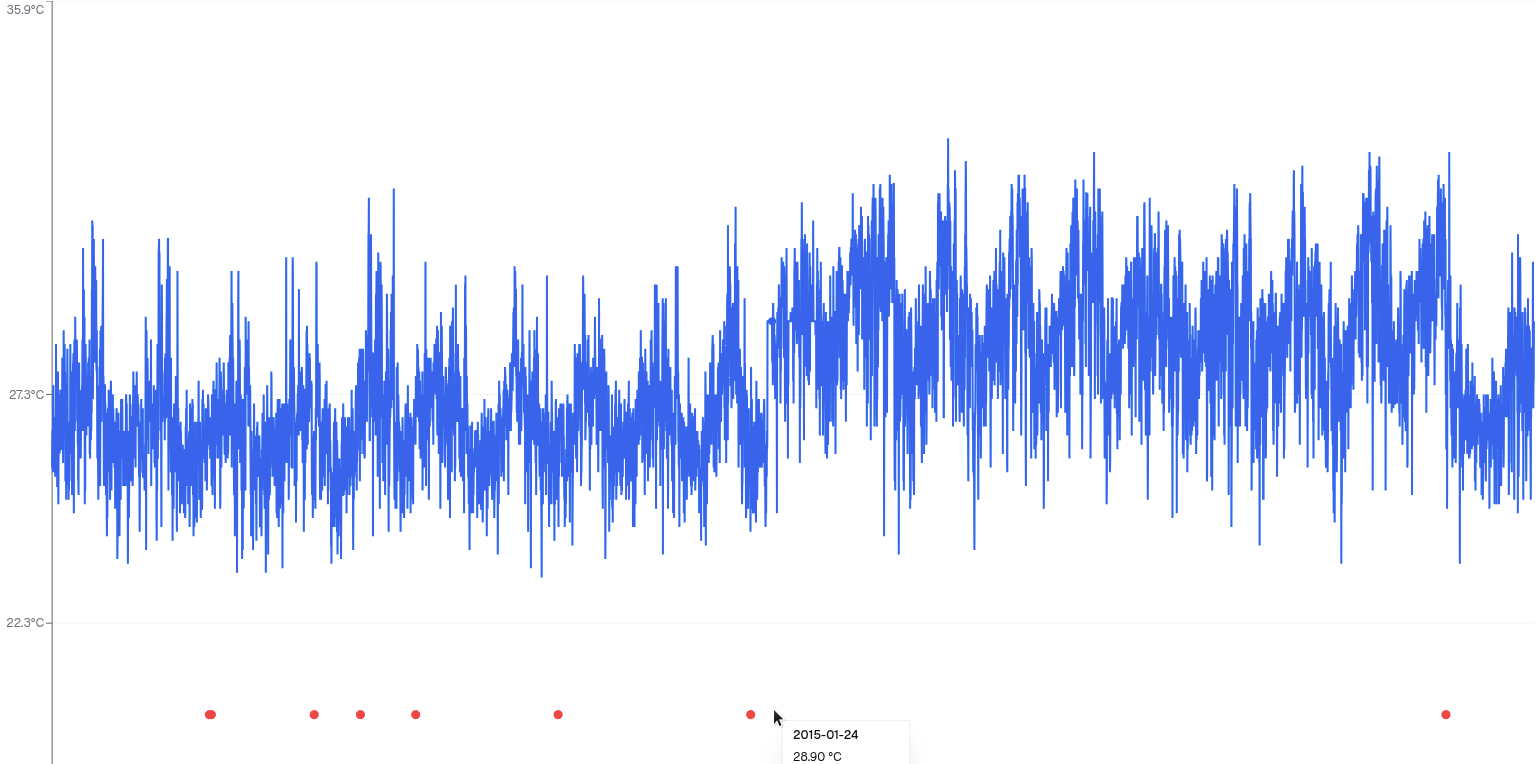
\includegraphics[width=0.8\linewidth]{image/bab4/preprocessing_bmkg/tavg_original.png}
                        \caption{Visualisasi awal \textit{Time-Series} Suhu Rata-rata (TAVG)}
                        \label{fig:tavg_original}
                \end{figure}
                \begin{figure}[H]
                        \centering
                        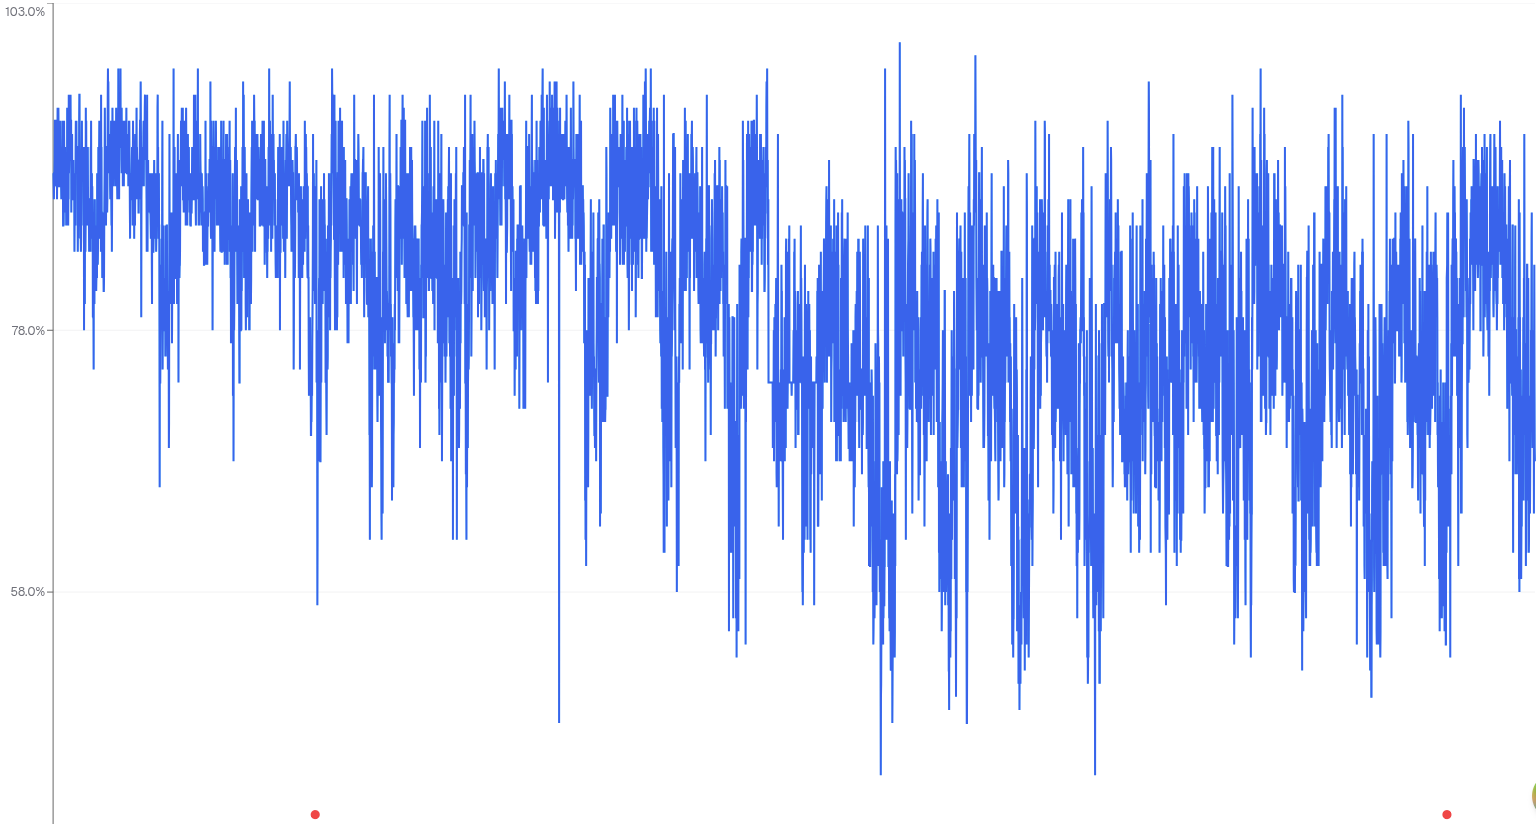
\includegraphics[width=0.8\linewidth]{image/bab4/preprocessing_bmkg/rhavg_original.png}
                        \caption{Visualisasi awal \textit{Time-Series} Kelembaban Relatif (RH\_AVG)}
                        \label{fig:rhavg_original}
                \end{figure}
                \begin{figure}[H]
                        \centering
                        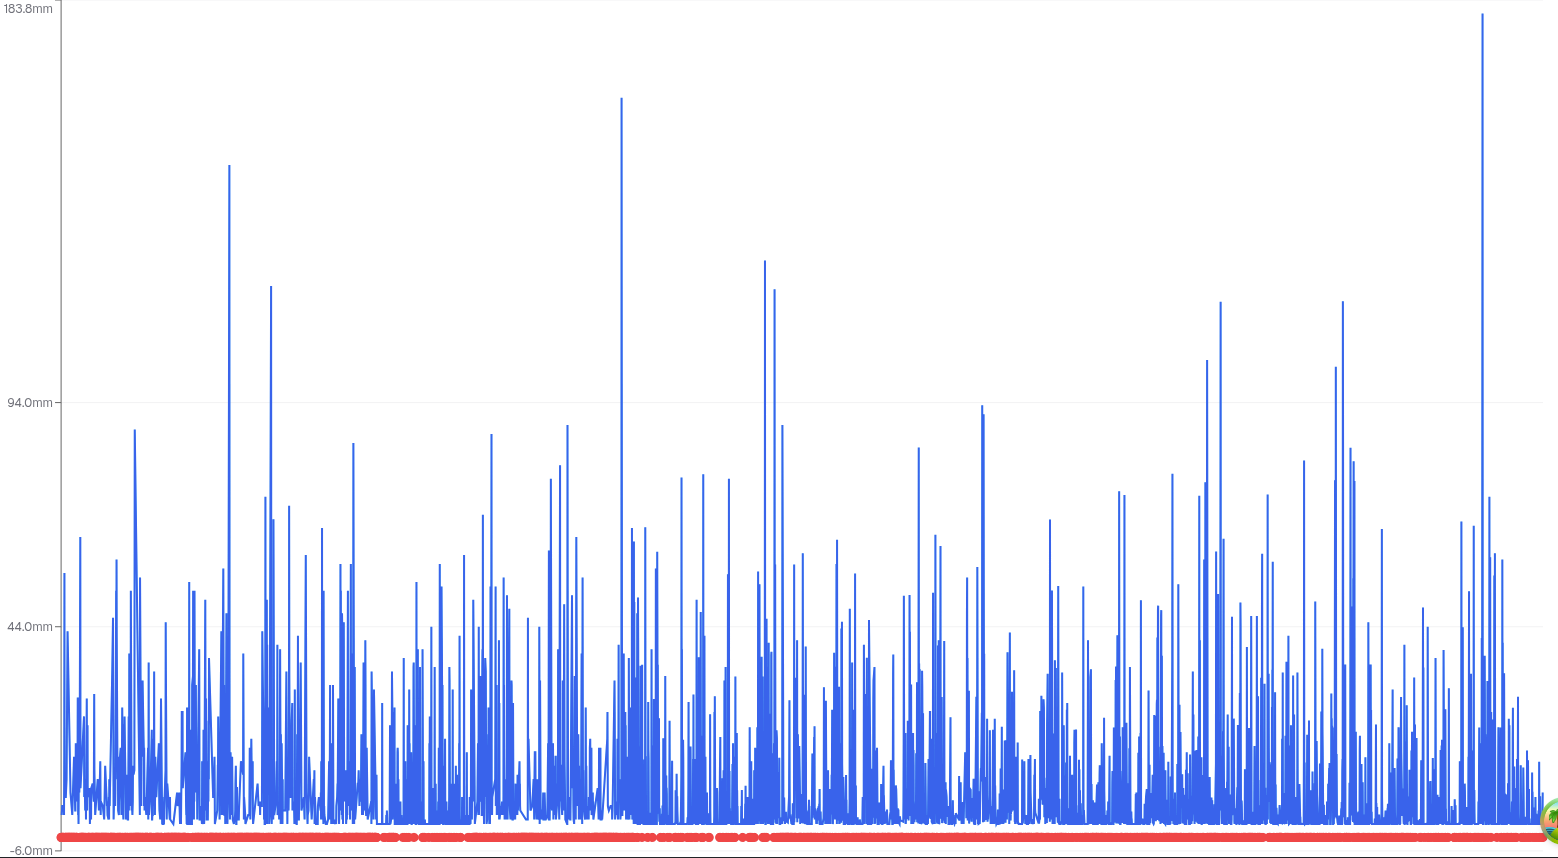
\includegraphics[width=0.8\linewidth]{image/bab4/preprocessing_bmkg/rr_original.png}
                        \caption{Visualisasi awal \textit{Time-Series} Curah Hujan (RR)}
                        \label{fig:rr_original}
                \end{figure}
            Variabel TAVG pada Gambar \ref{fig:tavg_original} menunjukkan pola suhu rata-rata harian yang relatif stabil dengan fluktuasi kecil. Meskipun terdapat 8 data invalid, distribusi data secara umum masih konsisten dan representatif terhadap kondisi suhu harian. Variabel RH\_AVG pada Gambar \ref{fig:rhavg_original} memperlihatkan pola kelembaban udara yang cenderung tinggi dan stabil. Hanya ditemukan 2 data invalid sehingga tidak memberikan pengaruh signifikan terhadap pola utama deret waktu. Namun, RR pada Gambar \ref{fig:rr_original} menunjukkan fluktuasi curah hujan yang sangat tinggi, sebanyak 2770 data invalid. Kondisi ini mengindikasikan perlunya proses imputasi lebih intensif agar pola curah hujan dapat digunakan secara optimal pada tahap pemodelan.
            
            \textbf{Imputasi dan Penanganan \textit{Outlier}} \\
            Proses imputasi dilakukan untuk menangani data invalid dan menjaga kontinuitas deret waktu. Metode imputasi yang digunakan disesuaikan dengan karakteristik masing-masing variabel, sedangkan outlier ditangani menggunakan interpolasi agar pola data tetap terjaga.
            \begin{table}[H]
                \centering
                \caption{Hasil Imputasi Data BMKG untuk Variabel Utama}
                \label{tab:bmkg_imputation}
                \scriptsize
                \setlength{\tabcolsep}{3pt} % padding antar kolom
                \renewcommand{\arraystretch}{1.2} % spasi vertikal
                \begin{tabularx}{\textwidth}{|l|p{4cm}|X|c|}
                \hline
                \textbf{Variabel} & \textbf{Metode Imputasi} & \textbf{Dasar Logika} & \textbf{Sisa \textit{Missing}} \\
                \hline
                TAVG (°C) &
                math\_relationships\_cubic\_spline &
                Dihitung bertahap: (1) hubungan matematis $TAVG=(TX+TN)/2$ jika TX dan TN tersedia; (2) \textit{cubic spline interpolation}; (3) median bulanan untuk sisa akhir &
                0 \\
                \hline
                RH\_AVG (\%) &
                dewpoint\_method\_cubic\_spline &
                Diestimasi bertahap: (1) RH dihitung dari hubungan suhu dan titik embun, $T_d \approx T - (100-RH)/5$; (2) \textit{cubic spline interpolation} &
                0 \\
                \hline
                RR (mm) &
                two\_stage\_binary\_conditional &
                Klasifikasi biner hujan/tidak-hujan menggunakan probabilitas musiman, \textit{Markov chain}, dan skor kelembapan-angin; jika "hujan", jumlah diestimasi dari median musiman. Kasus ambigu dibiarkan kosong &
                725 \\
                \hline
                \end{tabularx}
            \end{table}
            Berdasarkan Tabel \ref{tab:bmkg_imputation}, metode imputasi dipilih sesuai karakteristik masing-masing variabel iklim. Variabel TAVG dan RH\_AVG berhasil diimputasi sepenuhnya melalui pendekatan bertingkat (\textit{cascading}), yaitu memanfaatkan hubungan matematis antar-variabel, dilanjutkan dengan \textit{cubic spline interpolation}, serta median bulanan sebagai \textit{fallback} terakhir. Sebaliknya, variabel RR menggunakan metode \textit{two-stage binary conditional} karena karakteristik curah hujan bersifat fluktuatif dan tidak kontinu. Metode ini menentukan status hujan atau tidak hujan berdasarkan probabilitas musiman, \textit{Markov chain}, serta kondisi kelembapan dan angin, kemudian mengestimasi besarnya curah hujan apabila terklasifikasi hujan. Untuk menjaga integritas pola curah hujan, nilai dengan tingkat keyakinan rendah tidak dipaksakan untuk diimputasi sehingga masih terdapat 725 data \textit{missing value} pada variabel RR. \\
            \textbf{Hasil \textit{Smoothing}} \\
                \begin{figure}[H]
                        \centering
                        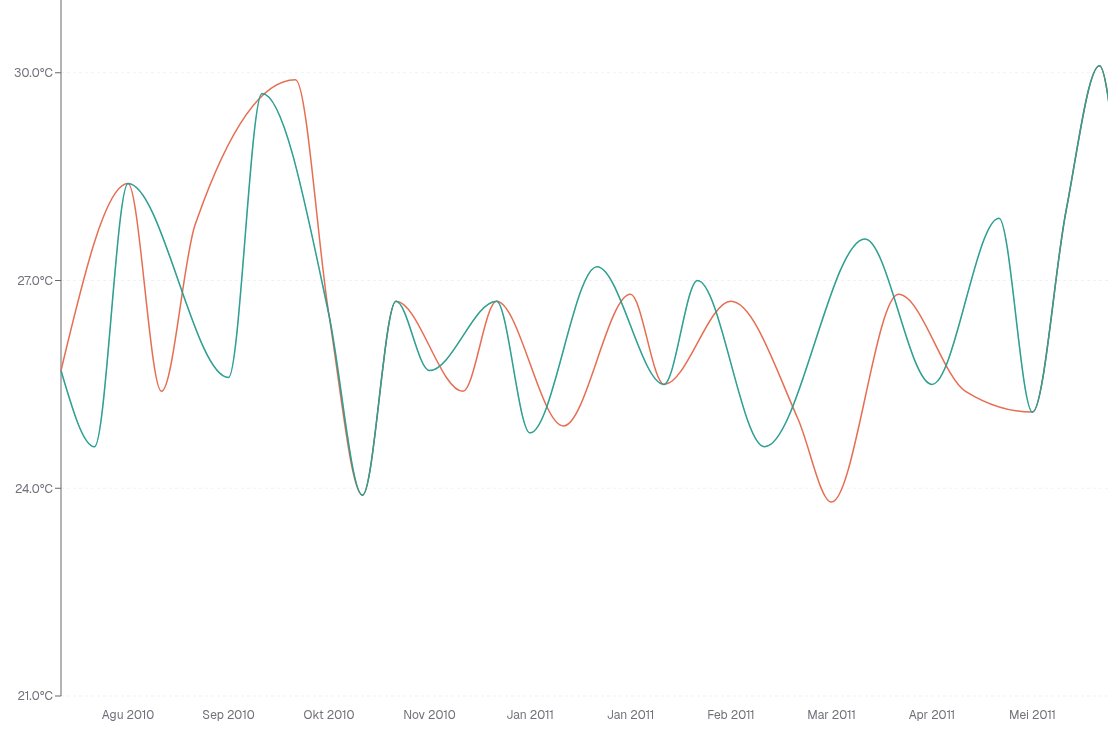
\includegraphics[width=0.8\linewidth]{image/bab4/preprocessing_bmkg/tavg_before_after.png}
                        \caption{Perbandingan Suhu Sebelum dan Sesudah \textit{Smoothing}}
                        \label{fig:tavg_before_after}
                \end{figure}
                \begin{figure}[H]
                        \centering
                        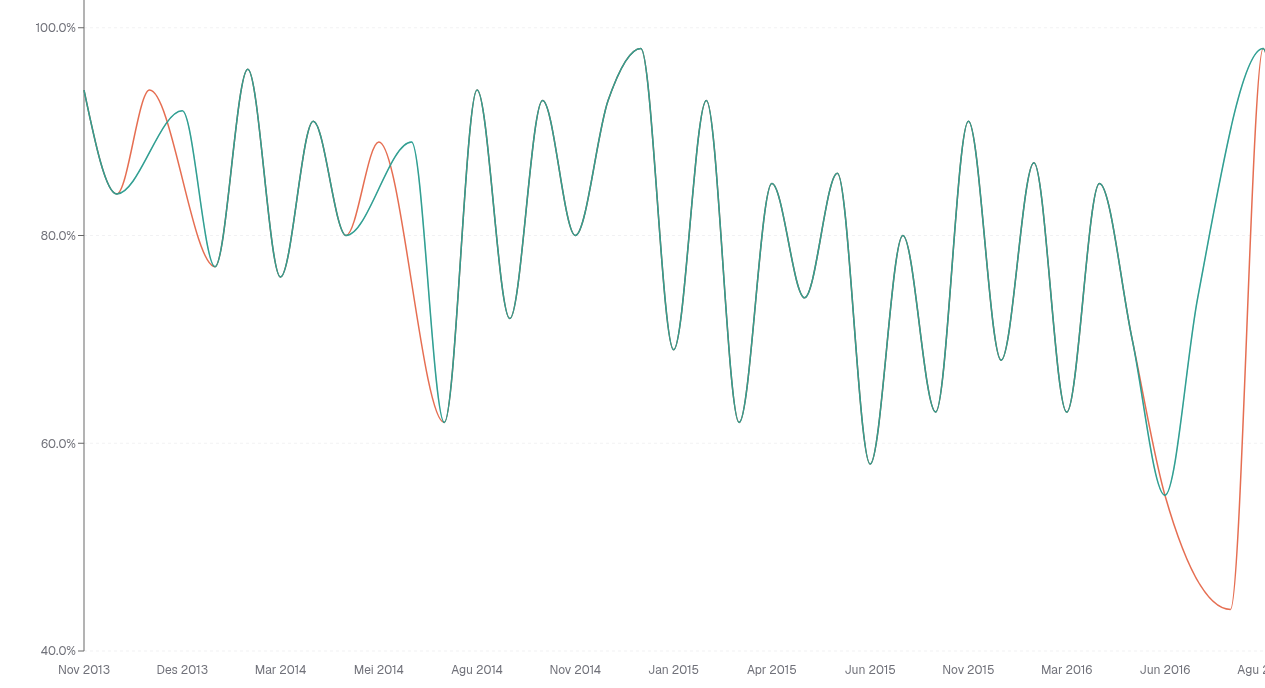
\includegraphics[width=0.8\linewidth]{image/bab4/preprocessing_bmkg/rhavg_before_after.png}
                        \caption{Perbandingan Kelembaban Sebelum dan Sesudah \textit{Smoothing}}
                        \label{fig:rhavg_before_after}
                \end{figure}
                \begin{figure}[H]
                        \centering
                        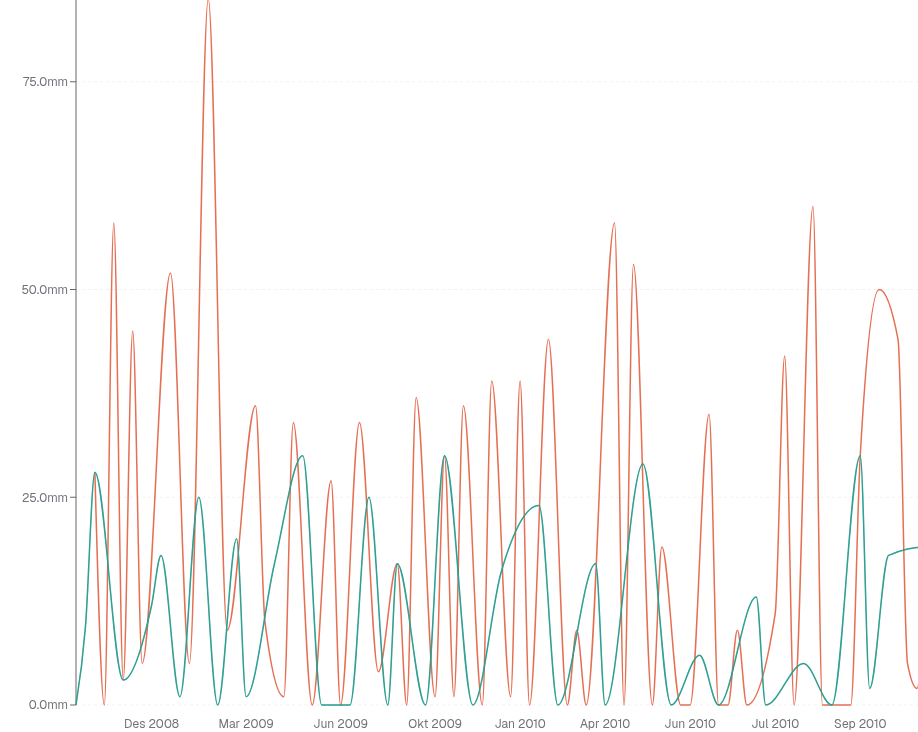
\includegraphics[width=0.8\linewidth]{image/bab4/preprocessing_bmkg/rr_before_after.png}
                        \caption{Perbandingan Curah Hujan Sebelum dan Sesudah \textit{Smoothing}}
                        \label{fig:rr_before_after}
                \end{figure}
                Visualisasi pada Gambar \ref{fig:tavg_before_after}, \ref{fig:rhavg_before_after}, dan \ref{fig:rr_before_after} menunjukkan bahwa proses \textit{smoothing} berhasil mengurangi noise dan fluktuasi tidak wajar tanpa menghilangkan pola utama masing-masing variabel. TAVG dan RH\_AVG memperlihatkan pola lebih stabil, sedangkan RR tetap mempertahankan karakteristik curah hujan yang fluktuatif namun dengan distribusi representatif setelah pembersihan data. Penambahan fitur \textit{brush} pada UI dan algoritma \textit{Largest Triangle Three Buckets} (LTTB) memungkinkan visualisasi rentang waktu tertentu dilakukan lebih fleksibel tanpa menghilangkan pola utama data. \\
            \textbf{Dekomposisi \textit{Time-Series}}
                \begin{figure}[H]
                        \centering
                        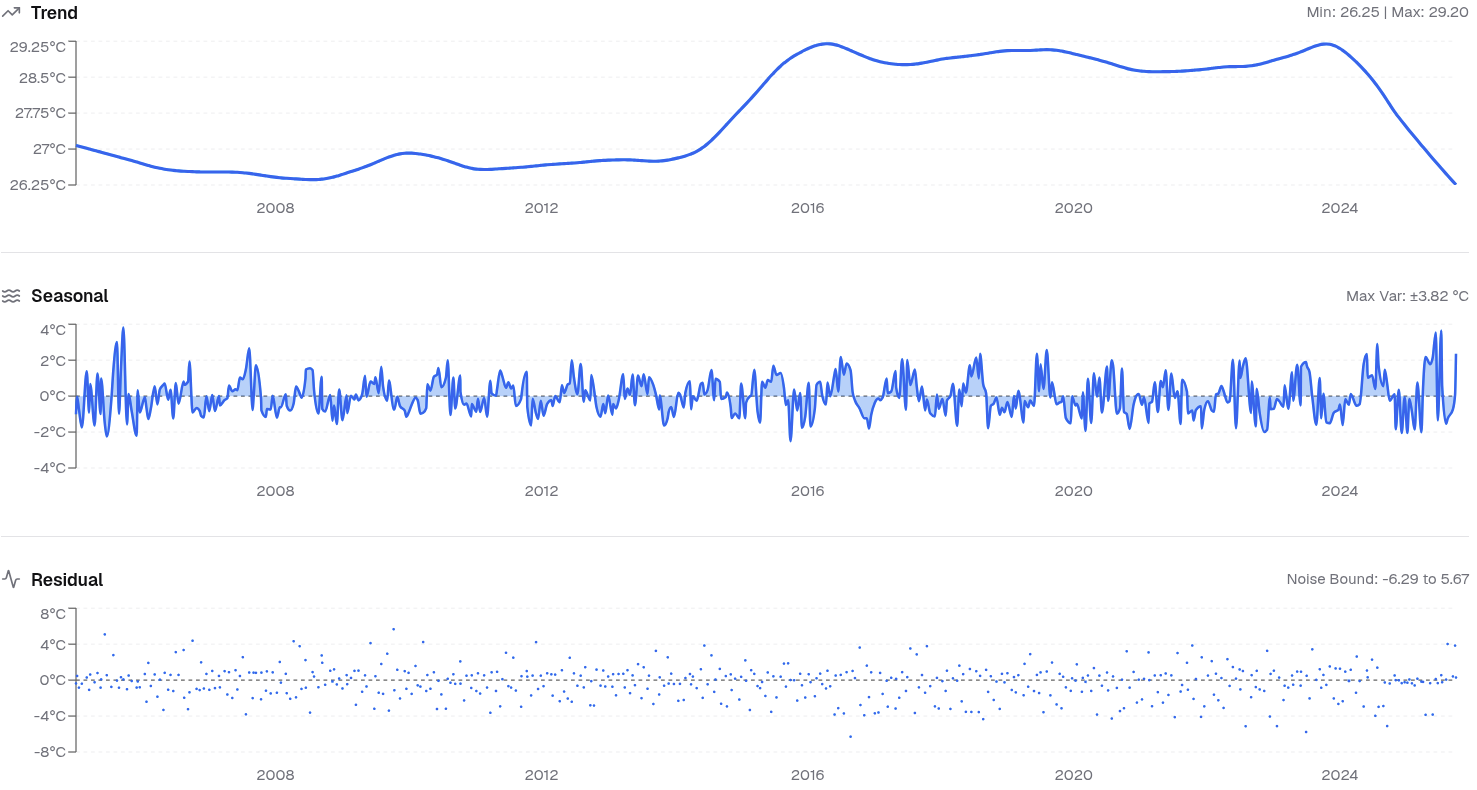
\includegraphics[width=0.8\linewidth]{image/bab4/preprocessing_bmkg/decomposition_tavg.png}
                        \caption{Dekomposisi Suhu rata-rata}
                        \label{fig:decomposition_tavg}
                \end{figure}
                \begin{figure}[H]
                        \centering
                        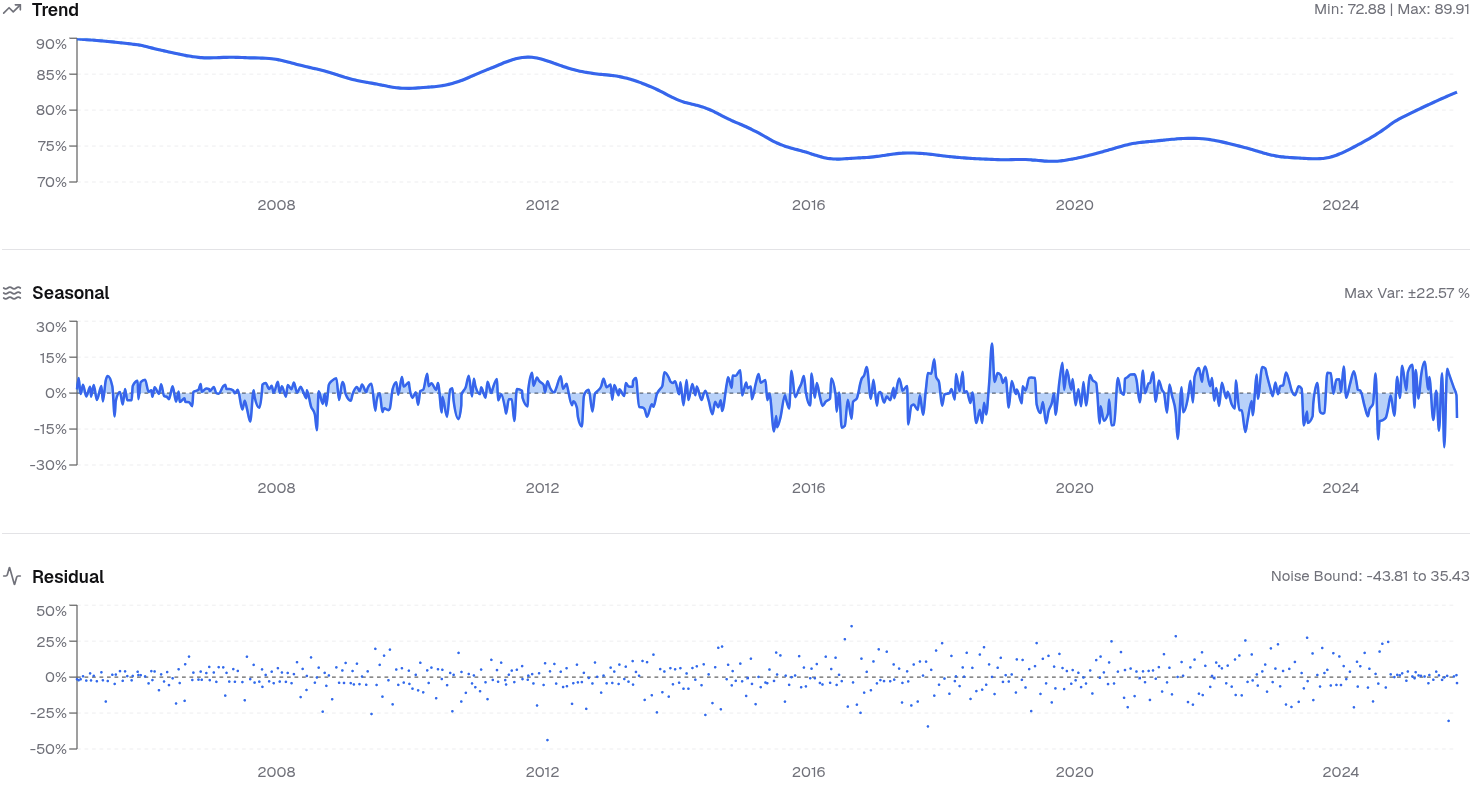
\includegraphics[width=0.8\linewidth]{image/bab4/preprocessing_bmkg/decomposition_rhavg.png}
                        \caption{Dekomposisi Kelembaban Relatif}
                        \label{fig:decomposition_rhavg}
                \end{figure}
                \begin{figure}[H]
                        \centering
                        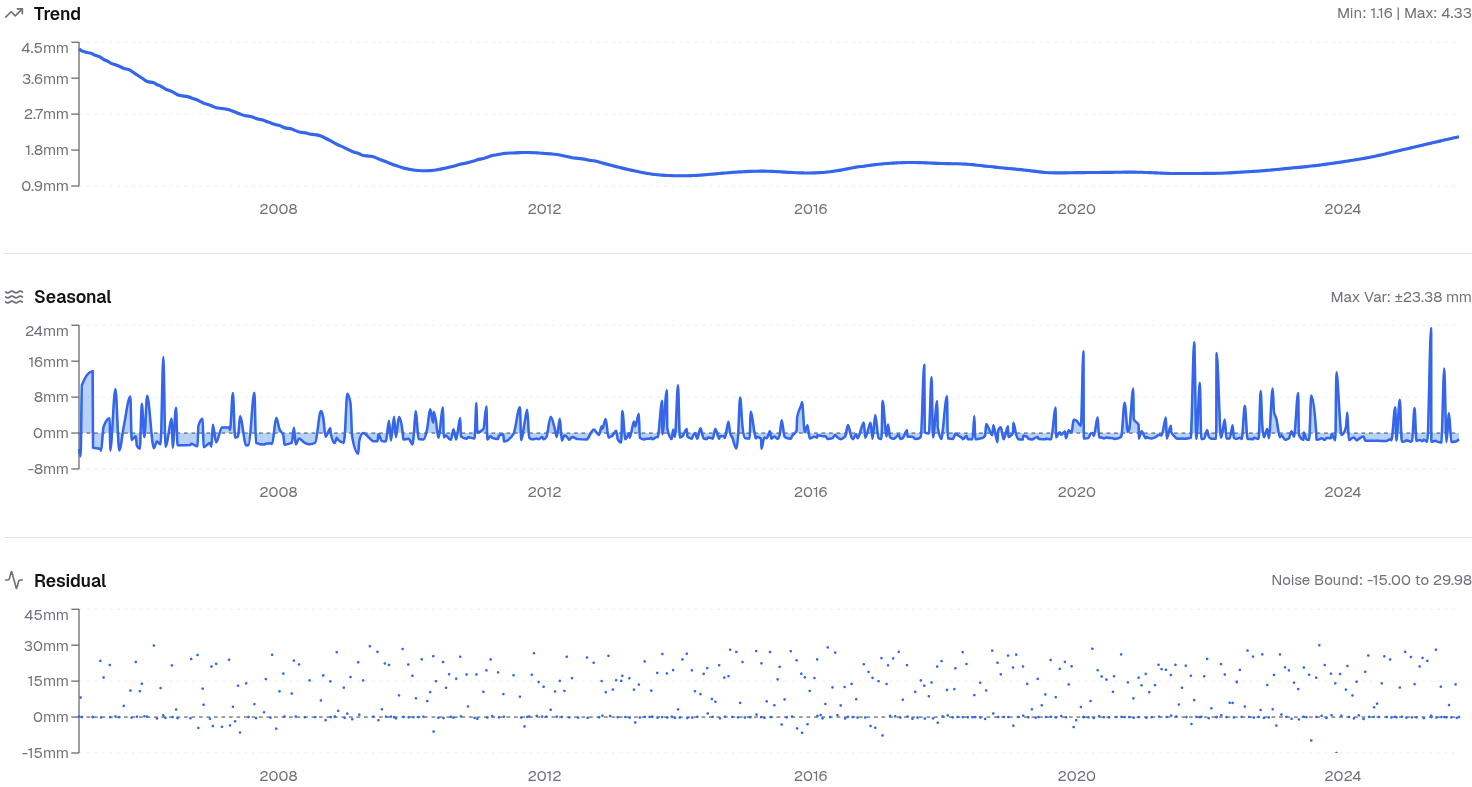
\includegraphics[width=0.8\linewidth]{image/bab4/preprocessing_bmkg/decomposition_rr.png}
                        \caption{Dekomposisi Curah Hujan}
                        \label{fig:decomposition_rr}
                \end{figure}
                Berdasarkan gambar \ref{fig:decomposition_tavg}, \ref{fig:decomposition_rhavg}, dan \ref{fig:decomposition_rr} Hasil dekomposisi STL pada data BMKG setelah \textit{preprocessing} menunjukkan tiga komponen: tren, musiman, dan residual. Untuk TAVG, tren memperlihatkan kenaikan tajam pada 2014–2018, puncak sekitar 2020, kemudian menurun. Komponen musiman konsisten berosilasi ±3–4 °C sesuai siklus tahunan. RH\_AVG menunjukkan tren menurun perlahan hingga 2018 lalu meningkat, dengan variasi musiman ±22\% mencerminkan siklus basah–kering. RR memiliki tren menurun hingga 2012 lalu relatif stabil, variasi musiman besar (±23 mm) menandakan dominasi hari kering diselingi hujan ekstrem. Visualisasi menggunakan \textit{downsampling} LTTB untuk meningkatkan waktu \textit{loading data}.
            \item \textbf{\textit{Dataset} NASA POWER} \\
            \textbf{Kondisi Awal \textit{Dataset}}
                \begin{figure}[H]
                        \centering
                        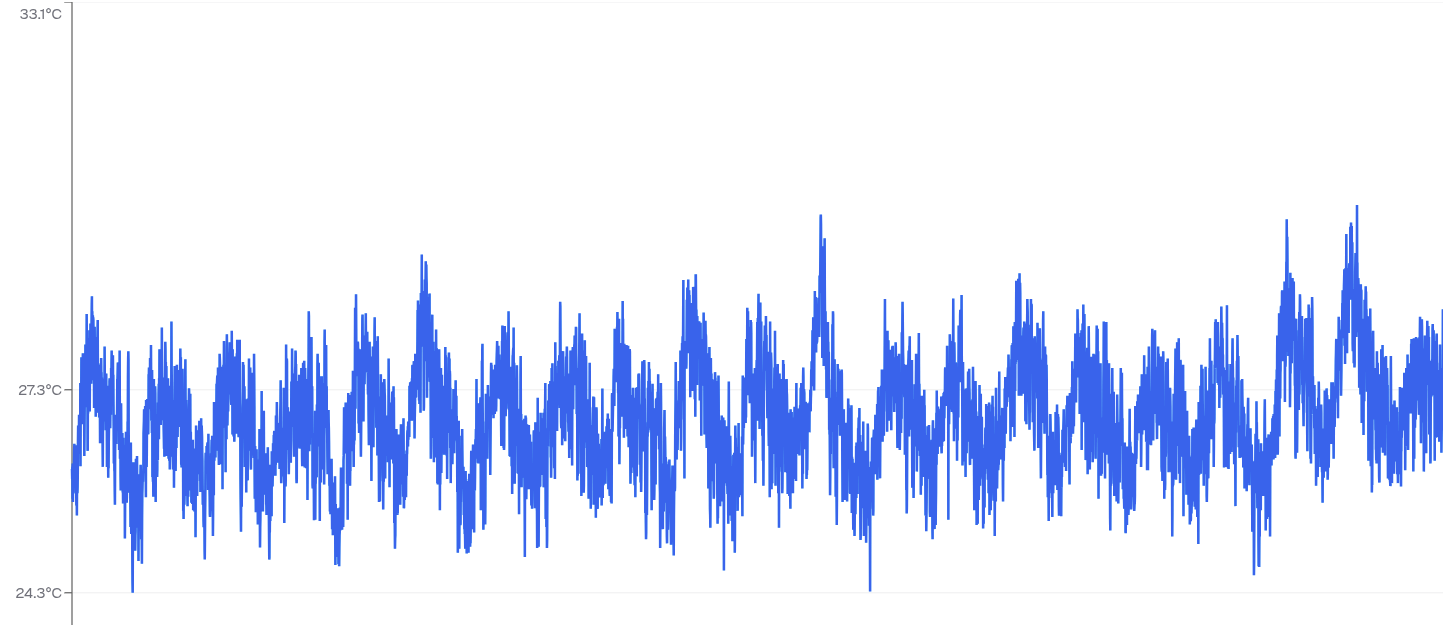
\includegraphics[width=0.8\linewidth]{image/bab4/preprocessing_nasa/t2m_original.png}
                        \caption{Visualisasi awal \textit{Time-Series} Suhu}
                        \label{fig:t2m_original}
                \end{figure}
                \begin{figure}[H]
                        \centering
                        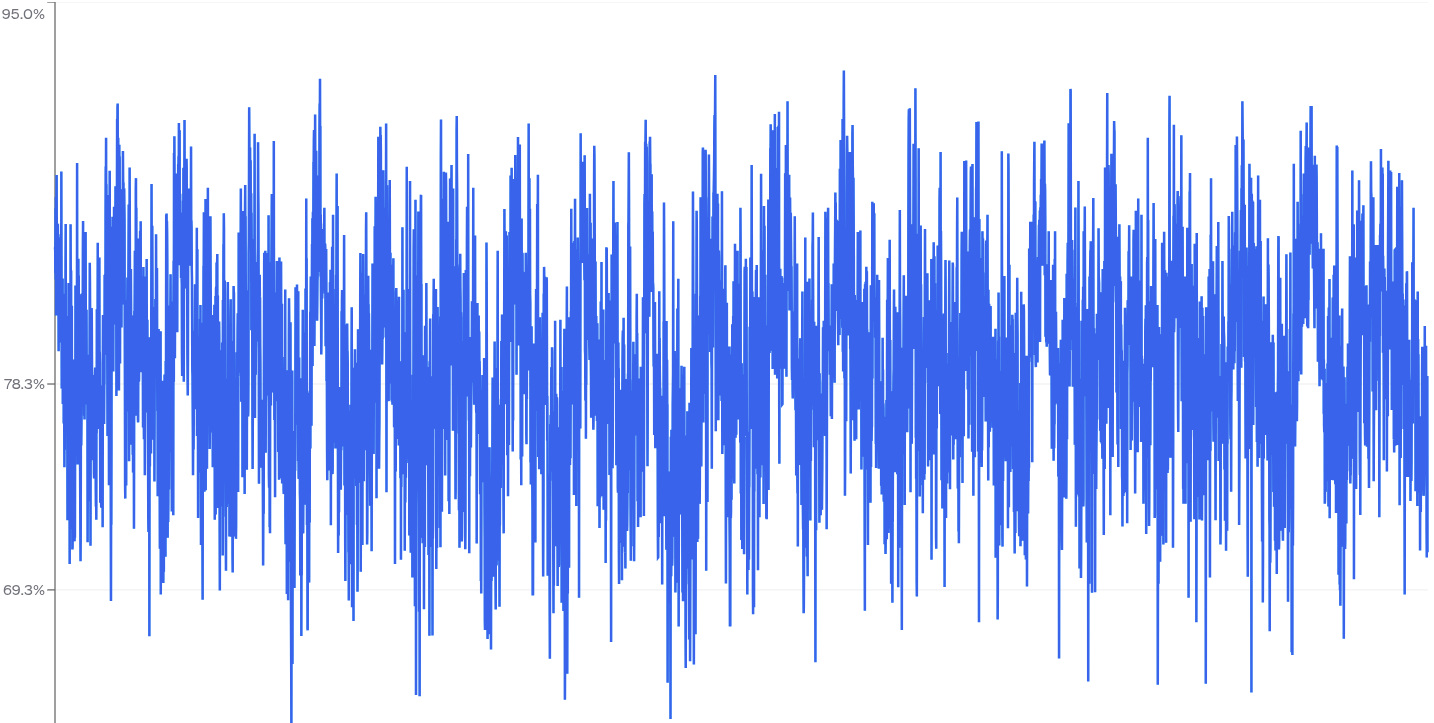
\includegraphics[width=0.8\linewidth]{image/bab4/preprocessing_nasa/rh2m_original.png}
                        \caption{Visualisasi awal \textit{Time-Series} Kelembaban}
                        \label{fig:rh2m_original}
                \end{figure}
                \begin{figure}[H]
                    \centering
                    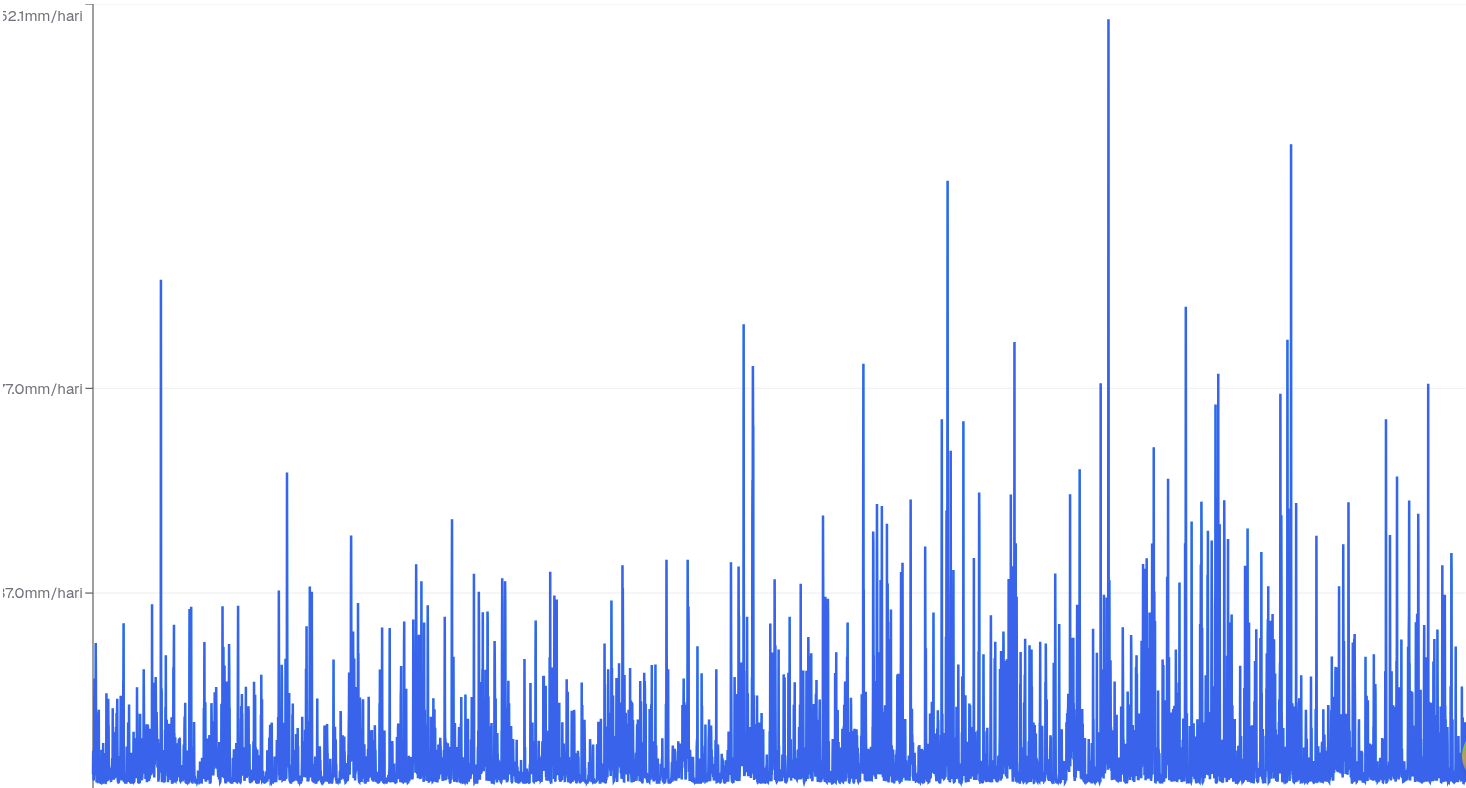
\includegraphics[width=0.8\linewidth]{image/bab4/preprocessing_nasa/prectotcorr_original.png}
                    \caption{Visualisasi awal \textit{Time-Series} Curah Hujan}
                    \label{fig:prectotcorr_original}
                \end{figure}

                \begin{figure}[H]
                    \centering
                    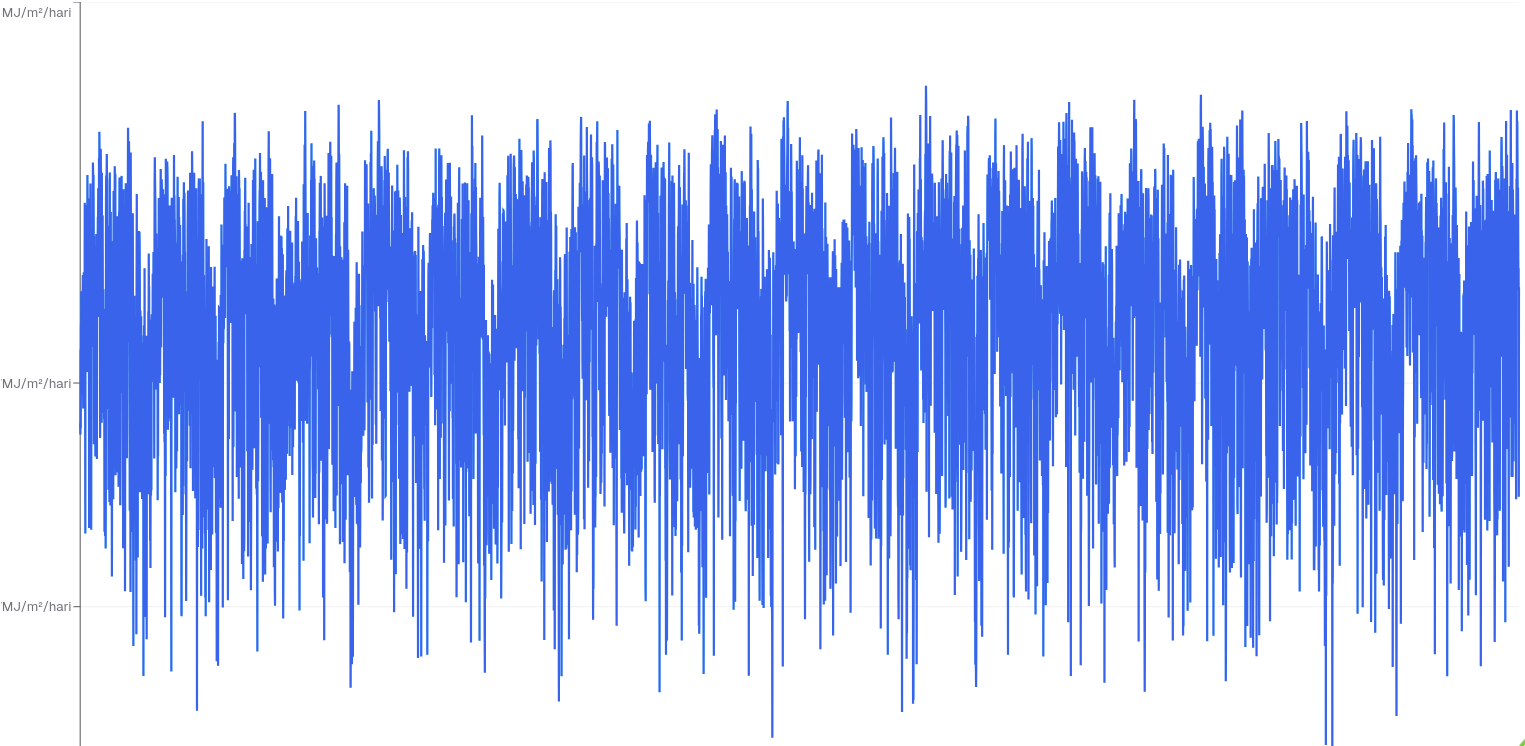
\includegraphics[width=0.8\linewidth]{image/bab4/preprocessing_nasa/all_sky_sfc_sw_dwn_original.png}
                    \caption{Visualisasi awal \textit{Time-Series} Radiasi Matahari}
                    \label{fig:all_sky_sfc_sw_dwn_original}
                \end{figure}
                Berdasarkan Gambar \ref{fig:t2m_original}, \ref{fig:rh2m_original}, \ref{fig:prectotcorr_original}, dan \ref{fig:all_sky_sfc_sw_dwn_original}, \textit{dataset} NASA POWER menunjukkan pola deret waktu yang relatif kontinu dan stabil tanpa ditemukan \textit{missing value}. Dibandingkan data BMKG, data NASA POWER memiliki noise rendah dan pola observasi lebih homogen, sehingga tahap \textit{preprocessing} lebih difokuskan pada proses \textit{smoothing} untuk meningkatkan konsistensi data. \\
            \textbf{Deteksi Outlier dan Hasil \textit{Smoothing}} \\
                \begin{table}[H]
                \centering
                \caption{Ringkasan Preprocessing NASA POWER untuk Variabel Utama}
                \label{tab:nasa_preprocessing}
                \small
                \begin{tabularx}{\linewidth}{|l|c|c|X|}
                \hline
                \textbf{Variabel} & \textbf{Outlier} & \textbf{\textit{Smoothing}} & \textbf{Keterangan} \\
                \hline
                T2M & 5 & Ya & \textit{Adaptive exponential smoothing} \\
                \hline
                RH2M & 2 & Ya & \textit{Adaptive exponential smoothing} \\
                \hline
                PRECTOTCORR & 0 & Tidak & Mempertahankan sinyal hujan ekstrem \\
                \hline
                ALLSKY\_SFC\_SW\_DWN & 0 & Tidak & Mempertahankan pola radiasi harian \\
                \hline
                \end{tabularx}
                \end{table}
                Berdasarkan Tabel \ref{tab:nasa_preprocessing}, \textit{dataset} NASA POWER tidak memiliki \textit{missing value}. Sebanyak 38 outlier terdeteksi (T2M: 5, T2M\_MIN: 23, RH2M: 2, WS10M: 2, WS10M\_MAX: 6), dengan outlier pada T2M\_MIN dan parameter angin berada di luar fokus utama. \textit{Smoothing} adaptif diterapkan pada T2M dan RH2M, sedangkan PRECTOTCORR dan ALLSKY\_SFC\_SW\_DWN tidak di-\textit{smoothing} untuk mempertahankan sinyal ekstrem dan variasi harian.
                \begin{figure}[H]
                        \centering
                        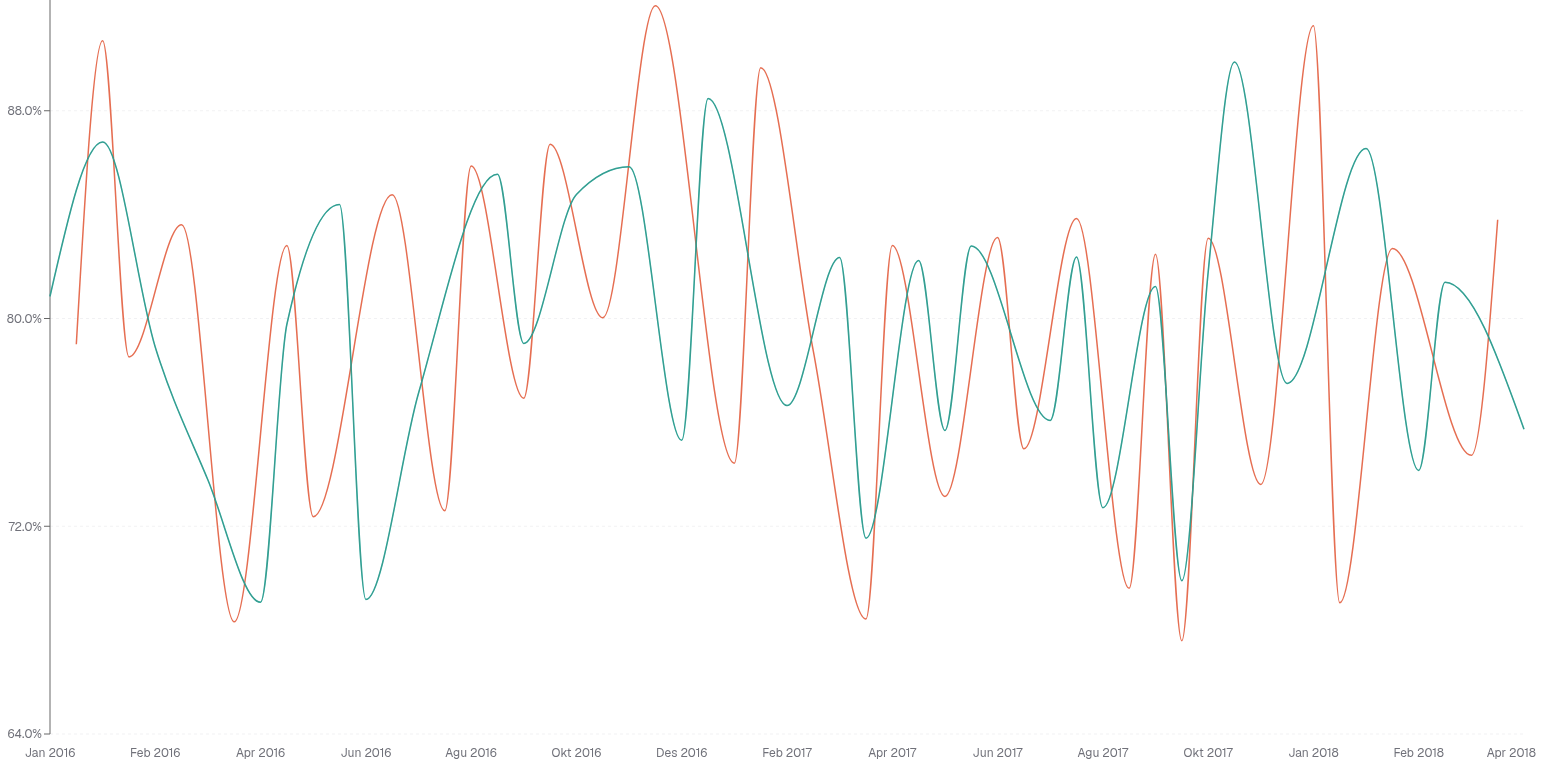
\includegraphics[width=0.8\linewidth]{image/bab4/preprocessing_nasa/rh2m_before_after.png}
                        \caption{Perbandingan Kelembaban Sebelum dan Sesudah \textit{Smoothing}}
                        \label{fig:rh2m_before_after}
                \end{figure}
                \begin{figure}[H]
                        \centering
                        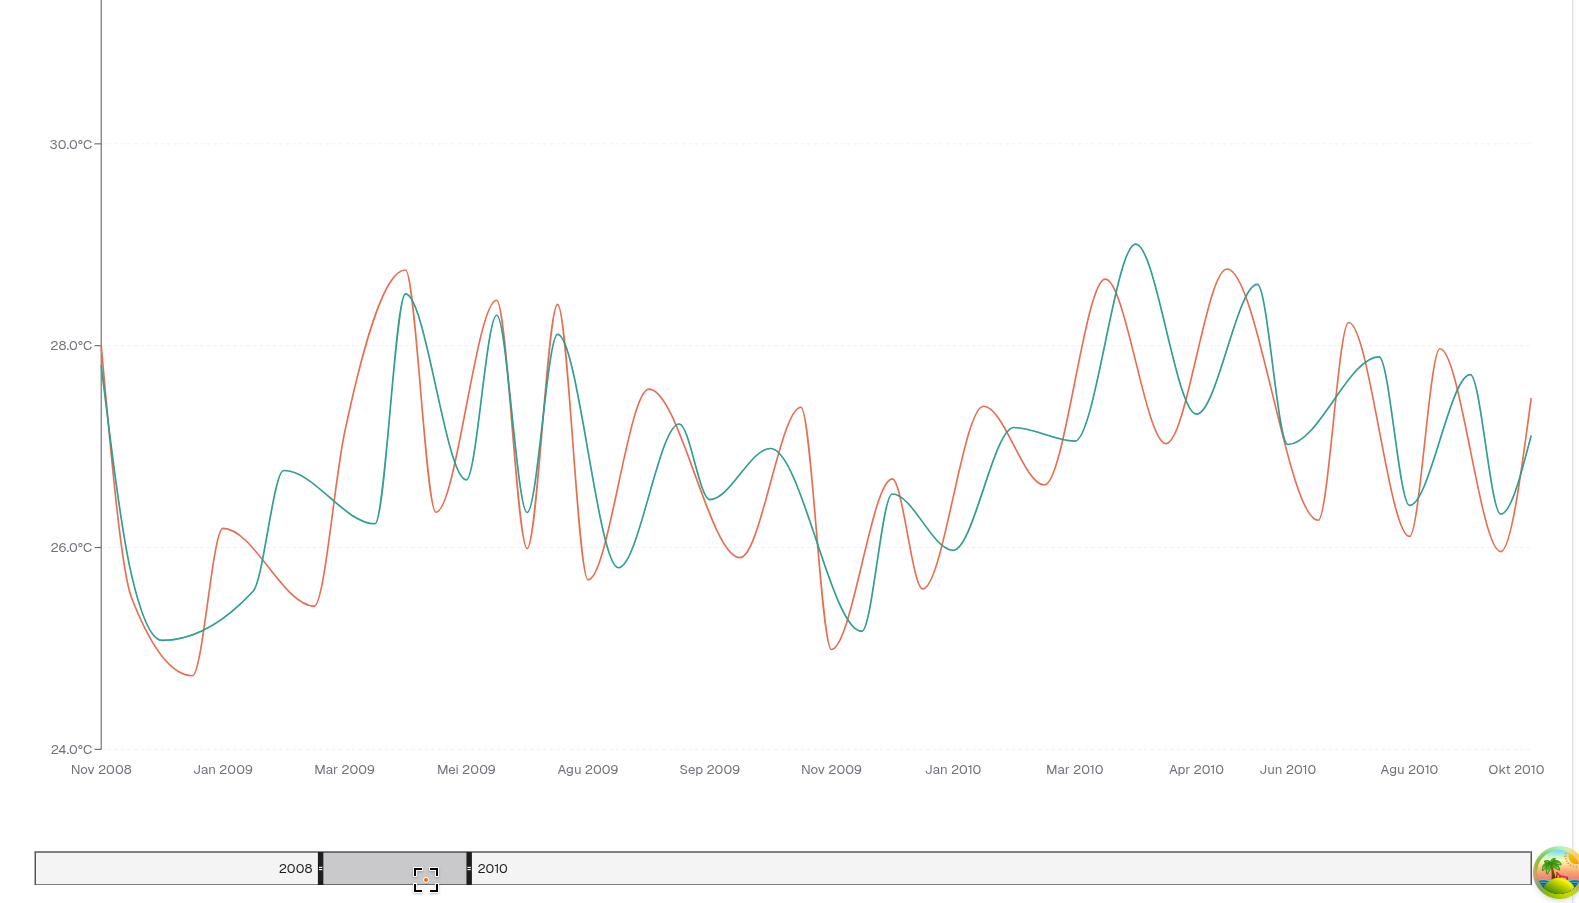
\includegraphics[width=0.8\linewidth]{image/bab4/preprocessing_nasa/t2m_before_after.png}
                        \caption{Perbandingan Suhu Sebelum dan Sesudah \textit{Smoothing}}
                        \label{fig:t2m_before_after}
                \end{figure}
                Visualisasi pada Gambar \ref{fig:rh2m_before_after} dan \ref{fig:t2m_before_after} menunjukkan bahwa proses \textit{smoothing} pada \textit{dataset} NASA POWER tidak mengubah pola utama data secara signifikan. Perbedaan antara data sebelum dan sesudah \textit{smoothing} relatif kecil karena \textit{dataset} NASA POWER sudah memiliki kualitas data yang stabil sejak awal. Proses \textit{smoothing} terutama berfungsi untuk memperbaiki fluktuasi pola tren. \\
            \textbf{Dekomposisi \textit{Time-Series}}
                \begin{figure}[H]
                        \centering
                        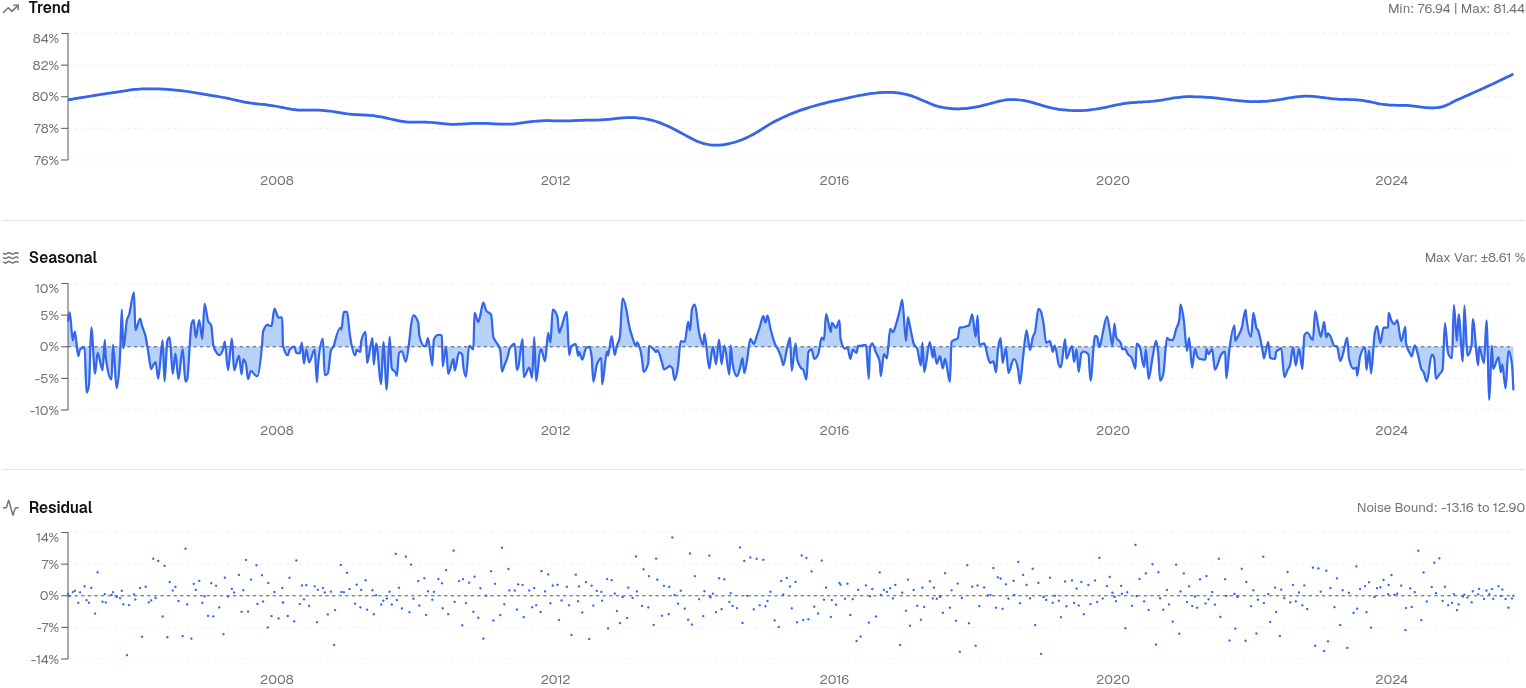
\includegraphics[width=0.8\linewidth]{image/bab4/preprocessing_nasa/decomposition_rh2m.png}
                        \caption{Dekomposisi \textit{Time-Series} Kelembaban}
                        \label{fig:decomposition_rh2m}
                \end{figure}
                \begin{figure}[H]
                        \centering
                        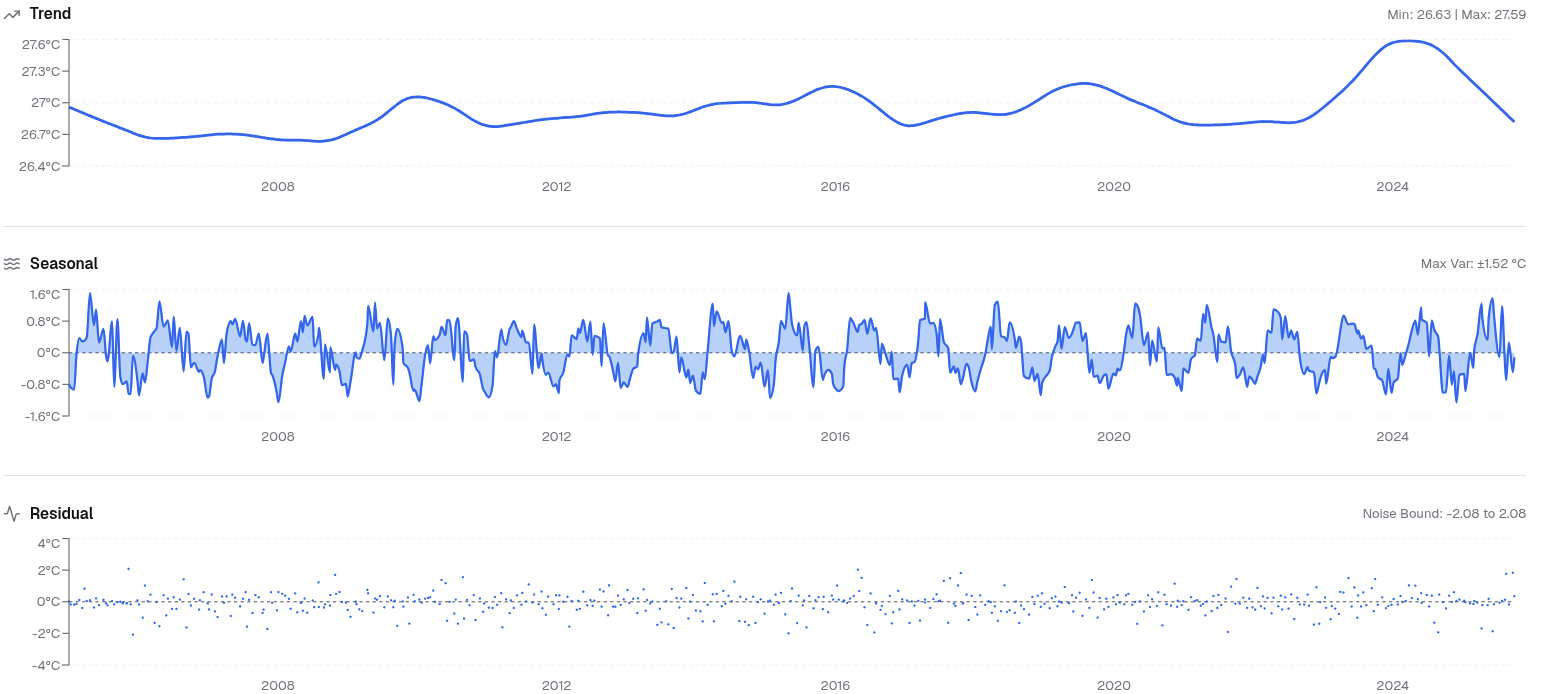
\includegraphics[width=0.8\linewidth]{image/bab4/preprocessing_nasa/decomposition_t2m.png}
                        \caption{Dekomposisi \textit{Time-Series} Suhu}
                        \label{fig:decomposition_t2m}
                \end{figure}
                \begin{figure}[H]
                        \centering
                        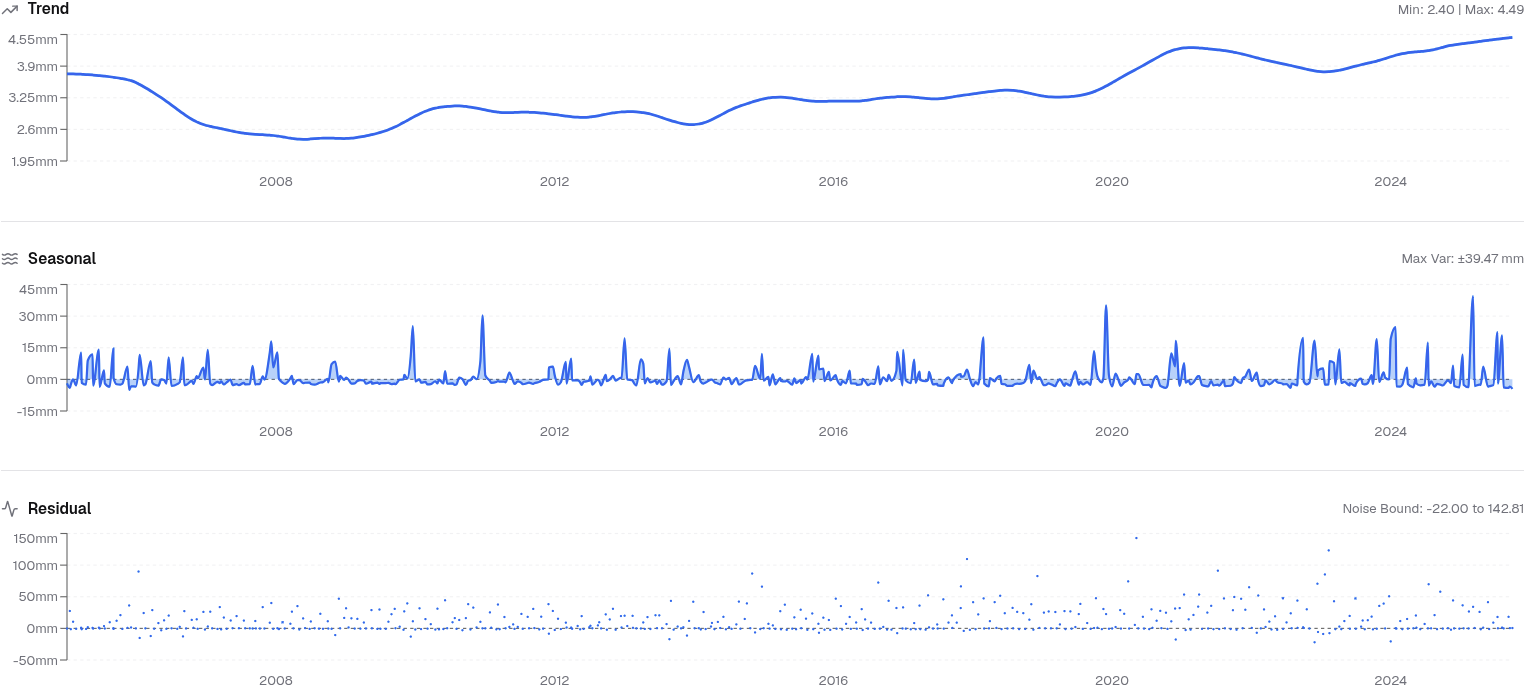
\includegraphics[width=0.8\linewidth]{image/bab4/preprocessing_nasa/decomposition_prectotcorr.png}
                        \caption{Dekomposisi \textit{Time-Series} Curah Hujan}
                        \label{fig:decomposition_prectotcorr}
                \end{figure}
                \begin{figure}[H]
                        \centering
                        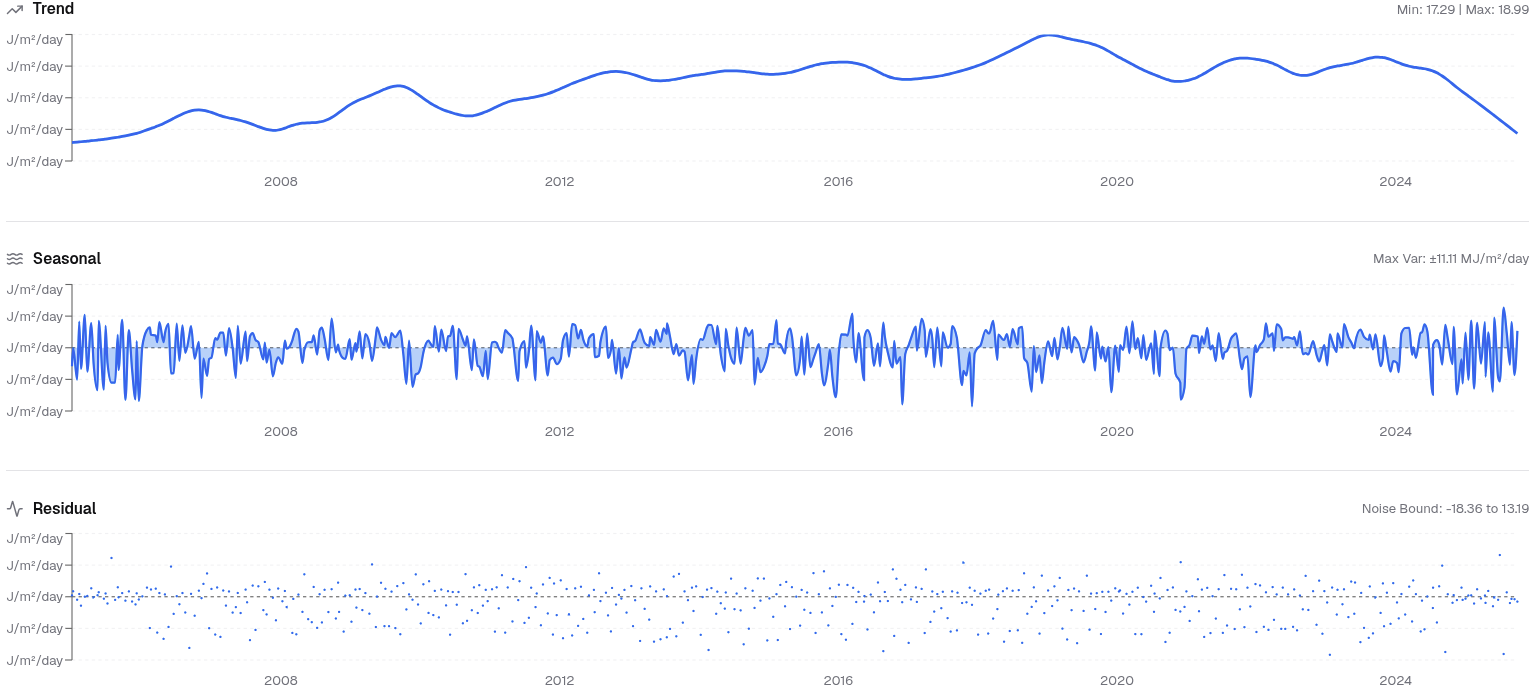
\includegraphics[width=0.8\linewidth]{image/bab4/preprocessing_nasa/decomposition_all_sky_sfc_sw_dwn.png}
                        \caption{Dekomposisi \textit{Time-Series} Radiasi Matahari}
                        \label{fig:decomposition_allsky_sfc_sw_dwn}
                \end{figure}
                Berdasarkan Gambar \ref{fig:decomposition_rh2m}, \ref{fig:decomposition_t2m}, \ref{fig:decomposition_prectotcorr}, dan \ref{fig:decomposition_allsky_sfc_sw_dwn}, dekomposisi NASA memberikan gambaran tren iklim yang cukup jelas dan konsisten. Pada variabel RH2M (kelembaban), tren jangka panjang menunjukkan penurunan perlahan hingga sekitar 2018 lalu kembali meningkat menuju 2025, dengan variasi musiman ±8–9\% yang mencerminkan siklus basah–kering tropis. Variabel T2M (suhu) relatif stabil, dengan tren bergerak di kisaran 26,6–27,6 °C, fluktuasi musiman kecil (±1,5 °C), dan residual yang rendah, menandakan iklim tropis homogen. Untuk PRECTOTCORR (curah hujan), tren menurun tajam sekitar 2008–2012 lalu stabil, dengan variasi musiman sangat besar (±39 mm) yang menegaskan dominasi hari kering diselingi hujan ekstrem. Sedangkan ALLSKY\_SFC\_SW\_DWN (radiasi matahari) menunjukkan tren fluktuatif dengan kisaran 17–19 MJ/m²/hari, variasi musiman tinggi (±11 MJ/m²/hari), serta residual yang cukup lebar akibat pengaruh atmosfer
    \end{enumerate}

\section{\textit{Deployment} Sistem}
Sistem yang dikembangkan telah diimplementasikan dalam lingkungan \textit{deployment} sehingga seluruh komponen dapat saling terintegrasi. Bagian \textit{frontend} di-\textit{deploy} menggunakan Vercel, sedangkan \textit{backend} pemrosesan data iklim dijalankan pada Ubuntu Server berbasis komputer lokal menggunakan Flask yang dioperasikan melalui Gunicorn sebagai \textit{WSGI server}. Layanan Flask dikonfigurasi sebagai \textit{system service} menggunakan \textit{systemd} sehingga dapat berjalan secara otomatis dan mendukung proses \textit{scheduler}, \textit{REST API}, serta pemrosesan model \textit{forecasting}. Seluruh metadata \textit{dataset}, hasil \textit{preprocessing}, log penjadwalan, dan autentikasi sistem disimpan pada MongoDB.
\begin{figure}[H]
    \centering
    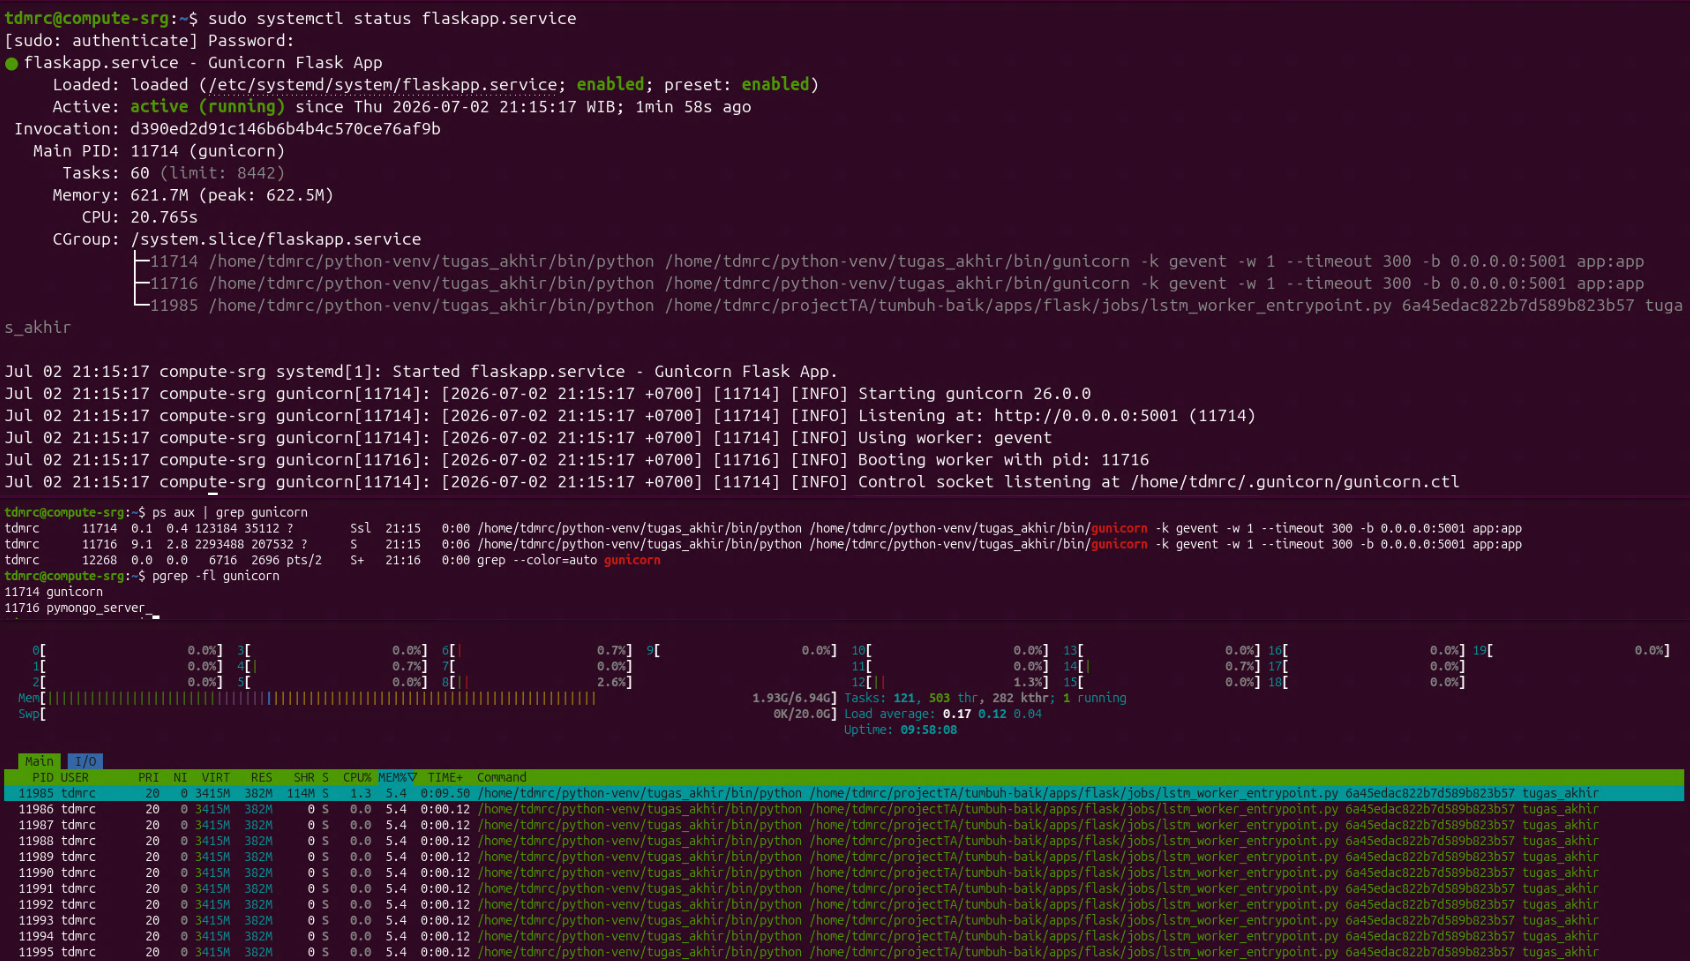
\includegraphics[width=0.9\linewidth]{image/bab4/deployment_tdmrc.png}
    \caption{Implementasi Layanan Flask Menggunakan Gunicorn pada Ubuntu Server}
    \label{fig:deployment_tdmrc}
\end{figure}
Implementasi layanan \textit{backend} ditunjukkan pada Gambar \ref{fig:deployment_tdmrc}. Gambar tersebut memperlihatkan bahwa layanan \textit{flaskapp.service} berstatus \textit{active (running)} melalui \textit{systemctl}, proses Gunicorn berhasil dijalankan sebagai \textit{worker} menggunakan perintah \textit{ps} dan \textit{pgrep}, serta proses \textit{forecasting} dan layanan Flask dapat dipantau melalui \textit{htop}. Hasil tersebut menunjukkan bahwa sistem berhasil diimplementasikan dan mampu beroperasi secara berkelanjutan pada Ubuntu Server.



\section{Pengujian Sistem}
Pengujian sistem dilakukan untuk memverifikasi bahwa \textit{frontend}, \textit{backend}, MongoDB, dan \textit{scheduler} terintegrasi dan memenuhi kriteria yang ditetapkan. Mengacu pada skenario pengujian pada Subbab 3.3.4, berikut disajikan hasil \textit{integration testing}, evaluasi kualitas data, maupun pengujian otomasi penjadwalan.
    \subsection{API \textit{Integration testing}}
        \begin{figure}[H]
            \centering
            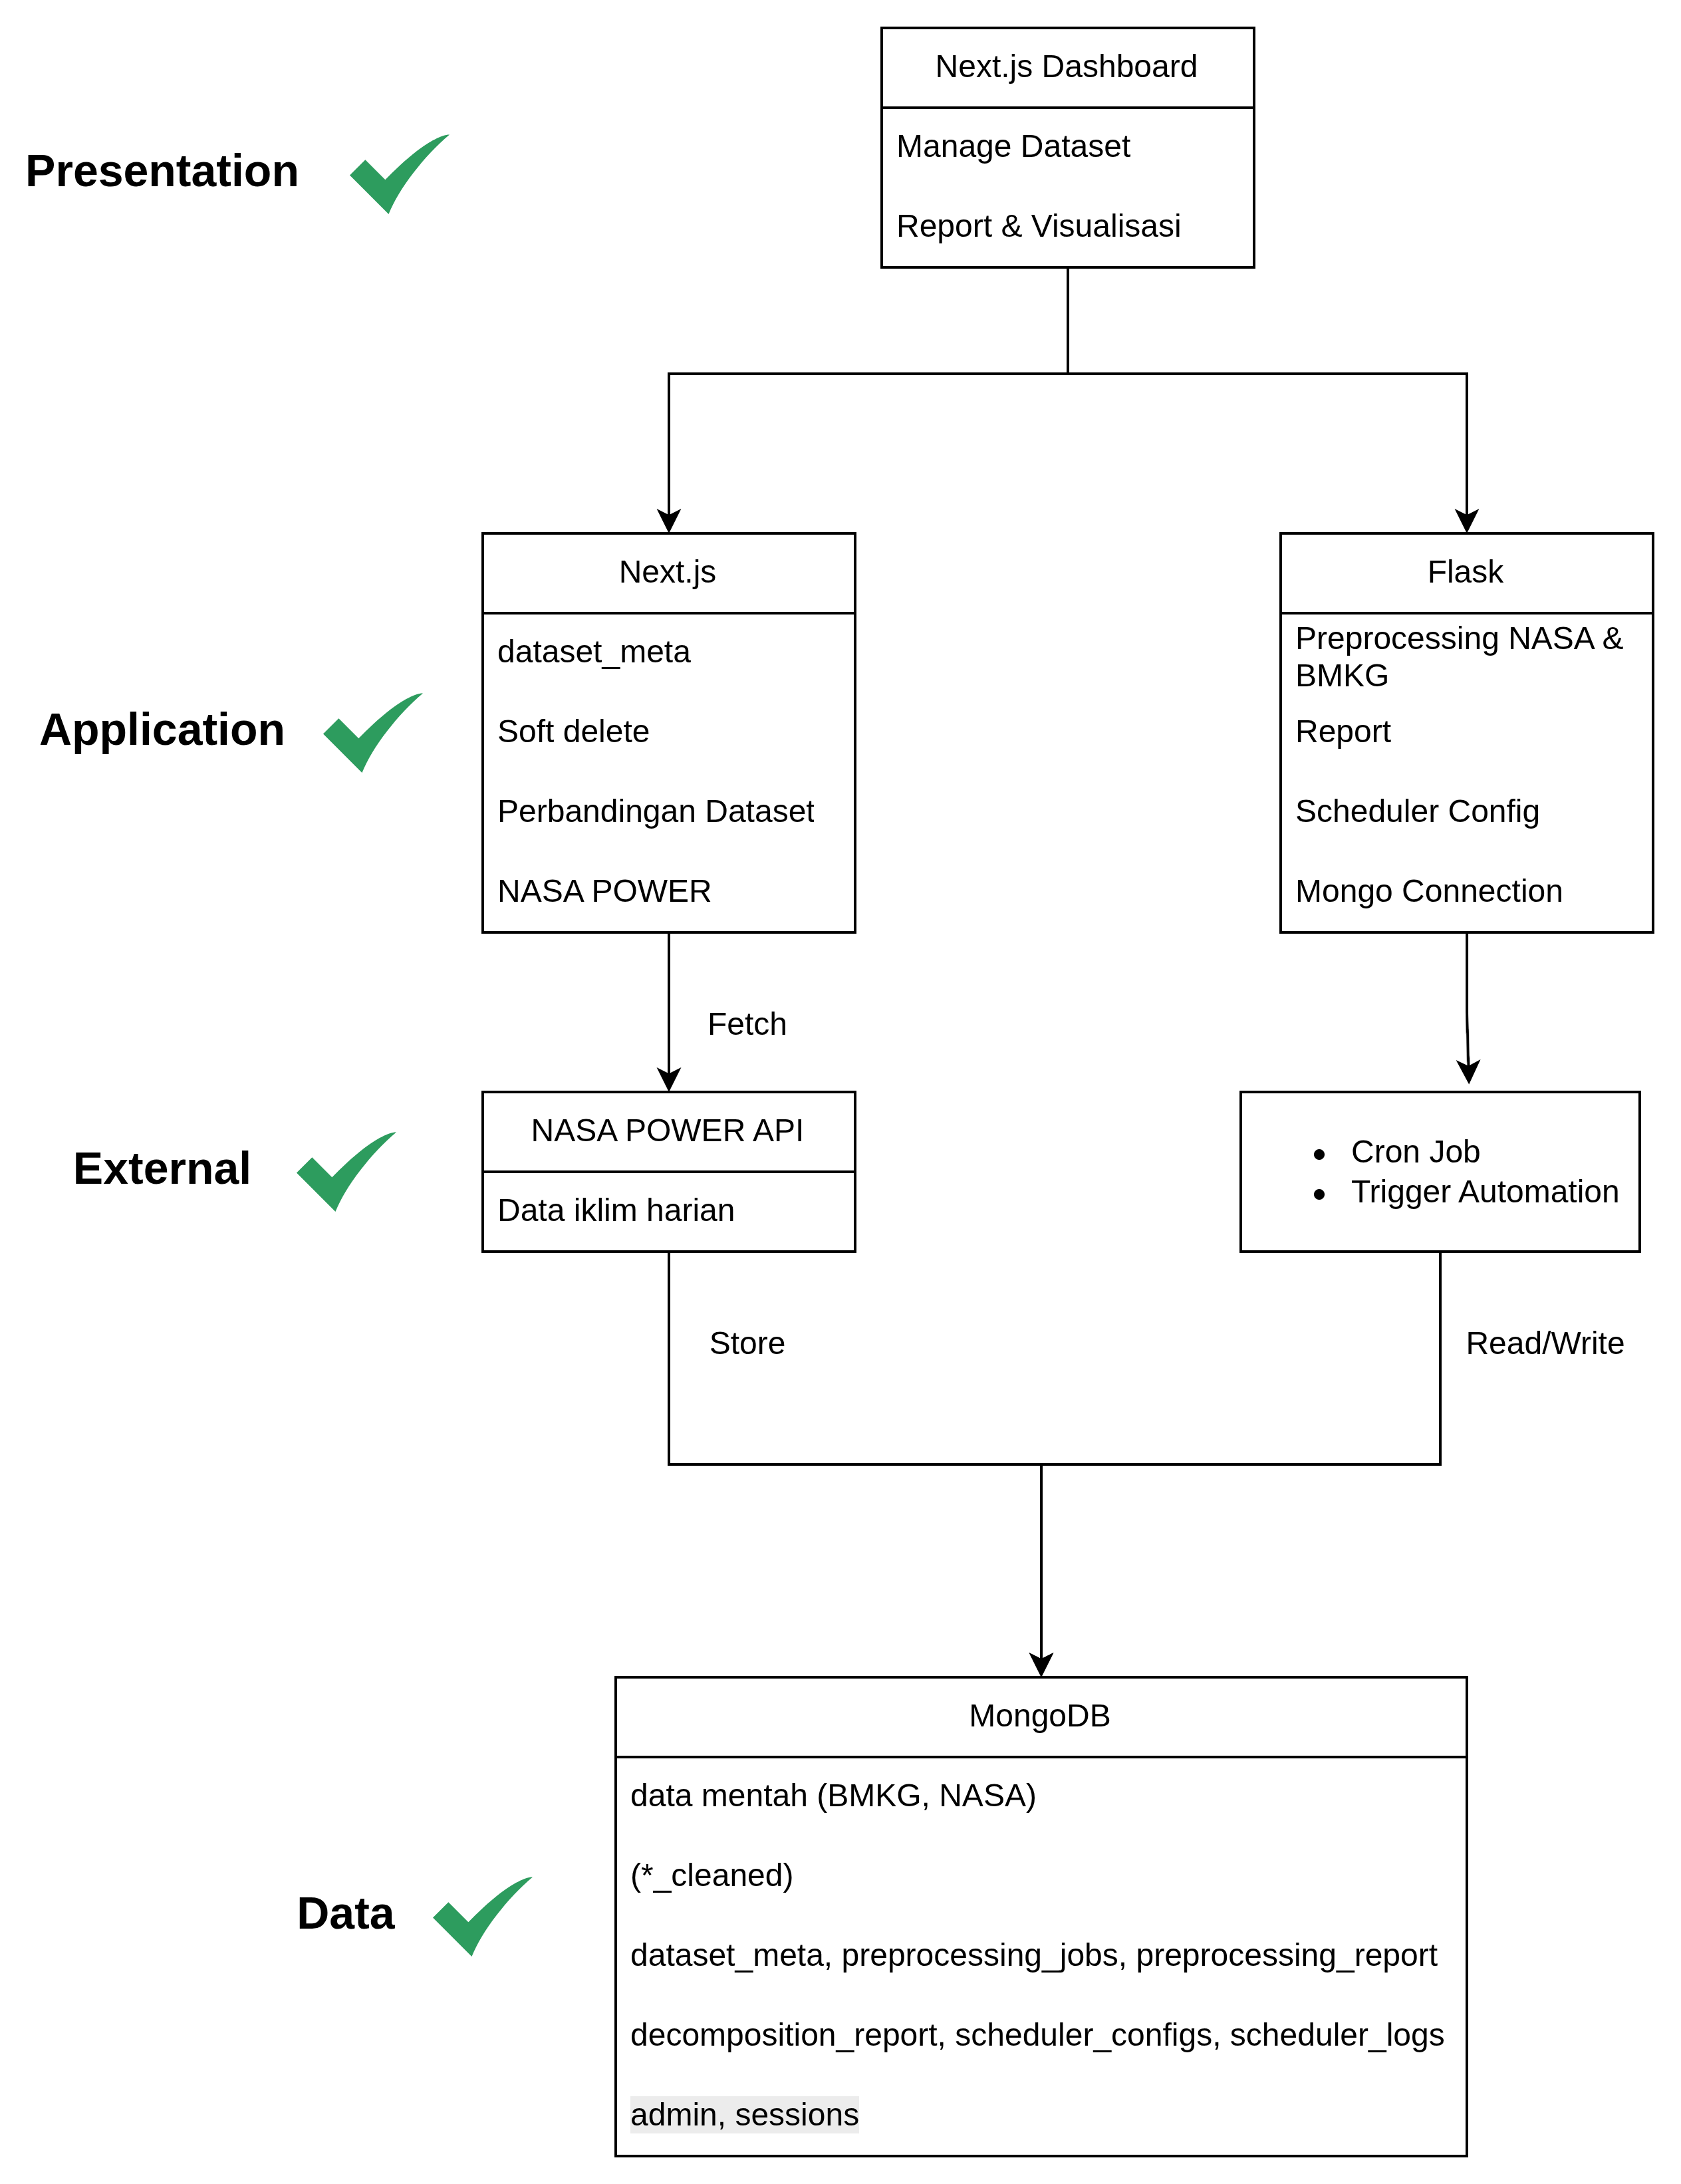
\includegraphics[width=0.6\linewidth]{image/bab4/alur_integrasi.png}
            \caption{Alur \textit{Integration Testing}}
            \label{fig:alur_integrasi}
        \end{figure}
        Hasil integrasi yang ditunjukkan pada Gambar \ref{fig:alur_integrasi} memperlihatkan bahwa setiap lapisan arsitektur berhasil terhubung. Pengujian komunikasi antara \textit{Presentation Layer} (Next.js Dashboard) dan \textit{Application Layer} (Next.js/Flask) berjalan lancar, \textit{request} antarmuka dapat diteruskan ke \textit{backend}. Integrasi dengan \textit{External Services Layer} (NASA POWER API) juga berhasil, ditandai dengan kemampuan backend melakukan fetching data secara konsisten. Pada \textit{Data Layer}, proses \textit{read-write} ke MongoDB tervalidasi dengan baik sehingga hasil request dapat tersimpan dan diakses kembali. \textit{End-to-end testing} menunjukkan alur lengkap dari input pengguna hingga data tersimpan di database dapat dijalankan. Adapun skenario pengujian akan dijelaskan pada tabel \ref{tab:integration_result_full} berikut. \\
        \begin{longtable}{|c|p{2.5cm}|>{\raggedright\arraybackslash}p{5.5cm}|c|p{3.5cm}|}
            \caption{Hasil Pengujian \textit{Integration Testing}} \label{tab:integration_result_full} \\
            \hline
            \textbf{No} & \textbf{Kelompok Pengujian} & \textbf{Endpoint} & \textbf{Hasil} & \textbf{Bukti Verifikasi} \\
            \hline
            \endfirsthead

            \multicolumn{5}{c}%
            {{Lanjutan Tabel \thetable}} \\
            \hline
            \textbf{No} & \textbf{Kelompok Pengujian} & \textbf{Endpoint} & \textbf{Hasil} & \textbf{Bukti Verifikasi} \\
            \hline
            \endhead

            \hline \multicolumn{5}{r}{Bersambung ke halaman berikutnya} \\
            \endfoot

            \hline
            \endlastfoot

            \scriptsize  % Font lebih kecil
            \setlength{\tabcolsep}{3pt}  % Kurangi padding antar kolom
                1 & \textit{Dataset Management} & GET /api/v1/datasets & $\checkmark$ & Semua dataset ditampilkan \\
                \hline
                2 & \textit{Dataset Management} & GET /api/v1/dataset/<slug> & $\checkmark$ & Koleksi berhasil diambil \\
                \hline
                3 & \textit{Connection Check} & GET /check-mongodb & $\checkmark$ & Status koneksi MongoDB OK \\
                \hline
                4 & \textit{Preprocessing} NASA & POST /api/v1/preprocess/nasa/<slug> & $\checkmark$ & Koleksi \_cleaned terbuat \\
                \hline
                5 & \textit{Preprocessing} BMKG & POST /api/v1/preprocess/bmkg/<slug> & $\checkmark$ & Koleksi \_cleaned terbuat \\
                \hline
                6 & \textit{Scheduler Status} & GET /api/v1/scheduler/status & $\checkmark$ & Status aktif ditampilkan \\
                \hline
                7 & \textit{Scheduler Logs} & GET /api/v1/scheduler/logs & $\checkmark$ & Log eksekusi tercatat \\
                \hline
                8 & \textit{Scheduler Config} & GET /api/v1/scheduler/config & $\checkmark$ & Konfigurasi ditampilkan \\
                \hline
                9 & \textit{Scheduler Config} & POST /api/v1/scheduler/config & $\checkmark$ & Konfigurasi baru tersimpan \\
                \hline
                10 & \textit{Scheduler Trigger} & POST /api/v1/scheduler/trigger & $\checkmark$ & Eksekusi manual berhasil \\
                \hline
                11 & NASA POWER API & GET power.larc.nasa.gov/api/pages & $\checkmark$ & API NASA diakses \\
                \hline
                12 & NASA POWER API & GET /api/temporal/daily/point? & $\checkmark$ & Data harian NASA POWER diambil \\
                \hline
                13 & \textit{Metadata Management} & GET /api/v1/dataset-meta/ & $\checkmark$ & Semua metadata ditampilkan \\
                \hline
                14 & NASA \textit{Refreshable} & GET /api/v1/nasa-power/refreshable & $\checkmark$ & List refreshable NASA \\
                \hline
                15 & \textit{Metadata Management} & GET /api/v1/dataset-meta/<slug> & $\checkmark$ & Metadata diambil \\
                \hline
                16 & NASA \textit{Refresh Single} & POST /api/v1/nasa-power/refresh/<id> & $\checkmark$ & Dataset NASA diperbarui \\
                \hline
                17 & NASA \textit{Refresh All} & POST /api/v1/nasa-power/refresh-all & $\checkmark$ & Semua dataset NASA diperbarui \\
                \hline
                18 & NASA \textit{Save Dataset} & POST /api/v1/nasa-power/save? & $\checkmark$ & Data NASA tersimpan ke MongoDB \\
                \hline
                19 & Metadata \textit{Update} & PATCH /api/v1/dataset-meta/<idOrSlug> & $\checkmark$ & Metadata berhasil di-edit \\
                \hline
                20 & Metadata \textit{Soft Delete} & PATCH /api/v1/dataset-meta/<slug>/delete & $\checkmark$ & \texttt{deletedAt} membuat data tidak muncul \\
                \hline
                21 & Metadata \textit{Restore} & PATCH /api/v1/dataset-meta/<slug>/restore & $\checkmark$ & Metadata dipulihkan \\
                \hline
                22 & Metadata \textit{Hard Delete} & DELETE /api/v1/dataset-meta/<slug> & $\checkmark$ & Metadata dan koleksi terkait terhapus \\
                \hline
                23 & \textit{Preprocessing Report} & GET /api/v1/preprocessing-report/<id> & $\checkmark$ & Laporan berhasil ditampilkan \\
                \hline
                24 & \textit{Decomposition} & GET /api/v1/preprocessing-report/<id>/decomposition & $\checkmark$ & Komponen tren, musiman, residual terisi \\
                \hline
                25 & \textit{Comparison} & GET /comparison/<original>/<cleaned> & $\checkmark$ & Perbandingan dua dataset original dan cleaned ditampilkan \\
                \hline
        \end{longtable}
        Tabel \ref{tab:integration_result_full} menyajikan hasil pengujian integrasi terhadap 25 \textit{endpoint} yang mencakup manajemen dataset, \textit{preprocessing} BMKG/NASA, penjadwalan, serta komunikasi dengan API eksternal NASA POWER. Seluruh \textit{endpoint} berhasil dijalankan, dibuktikan dengan kemampuan sistem dalam menyimpan metadata, membentuk koleksi \textit{cleaned}, menghasilkan laporan \textit{preprocessing} dan dekomposisi, serta mengeksekusi \textit{scheduler} secara manual maupun otomatis. Keberhasilan ini menunjukkan bahwa integrasi antar \textit{frontend} (Next.js), \textit{backend} (Flask/Next.js), MongoDB, dan layanan eksternal telah berfungsi sesuai kebutuhan sistem otomasi pemrosesan data iklim.
    \subsection{Pengujian Kualitas Data}
    Pengujian kualitas data dilakukan untuk mengevaluasi kualitas hasil \textit{preprocessing} berdasarkan tiga metrik: GCV (semakin kecil semakin baik), \textit{trend preservation} (persentase kemiripan arah tren), serta \textit{model coverage} untuk Holt-Winters (HW) dan LSTM. Hasil pengujian disajikan per sumber data. \\
    \noindent\textbf{Data BMKG} \\
    Tabel \ref{tab:bmkg_datatest} merangkum nilai GCV, \textit{trend preservation}, dan \textit{coverage} untuk tiga variabel utama BMKG: TAVG, RH\_AVG, dan RR.
    \begin{table}[H]
        \centering
        \caption{Hasil Pengujian Data BMKG}
        \label{tab:bmkg_datatest}
        \small
        \renewcommand{\arraystretch}{1.2}
        \setlength{\tabcolsep}{6pt}
        \begin{tabular}{|l|c|c|c|c|c|}
        \hline
        \textbf{Variabel} & \textbf{GCV} & \textbf{Trend(\%)} & \textbf{Status} & \textbf{HW(\%)} & \textbf{LSTM(\%)} \\
        \hline
        TAVG & 0,0006 & 99,92 & Excellent & 91,35 & 99,98 \\
        \hline
        RH\_AVG & 0,0009 & 99,94 & Excellent & 91,74 & 99,96 \\
        \hline
        RR & 1,3511 & 90,12 & Excellent & 77,87 & 79,43 \\
        \hline
        \end{tabular}
    \end{table}
    \begin{enumerate}[(a)]
        \item \textbf{Kualitas imputasi dan \textit{smoothing}}:  
        TAVG dan RH\_AVG memiliki GCV sangat rendah (<0,001) dan \textit{trend preservation} hampir sempurna (>99,9\%), menandakan bahwa metode \textit{mathematical relationships cubic spline} dan \textit{dewpoint cubic spline} berhasil mengisi nilai hilang tanpa merusak pola musiman. RR meskipun memiliki GCV 1,35 (masih kategori \textit{excellent}) dan \textit{trend preservation} 90\%, nilai tersebut lebih tinggi karena sifat curah hujan yang fluktuatif dan adanya 725 data yang sengaja tidak diimputasi (kelengkapan hanya 90,4\%).  

        \item \textbf{\textit{Forecasting coverage}}:
        HW/LSTM untuk TAVG dan RH\_AVG sangat tinggi (>91\% HW, >99\% LSTM), mengindikasikan kedua parameter siap untuk pemodelan. RR memiliki coverage lebih rendah (HW 77,9\%, LSTM 79,4\%), mencerminkan tantangan dalam meramalkan curah hujan akibat sebaran data yang tidak kontinu dan musiman lemah (seasonality strength 0,086).  

        \item \textbf{Karakteristik curah hujan (RR)}:  
        Meskipun GCV masih \textit{excellent}, sisa missing yang cukup besar (725 dari 7565) dan coverage yang hanya sekitar 78–79\% menegaskan bahwa RR memerlukan perlakuan khusus pada tahap pemodelan. Sistem merekomendasikan \textit{LSTM with caution} untuk parameter ini.
    \end{enumerate}
    \noindent\textbf{Data NASA POWER} \\
    Tabel \ref{tab:nasa_datatest} menyajikan hasil pengujian untuk empat variabel utama NASA: T2M, RH2M, PRECTOTCORR, dan ALLSKY\_SFC\_SW\_DWN. Perhatikan bahwa PRECTOTCORR dan ALLSKY tidak dilakukan smoothing (GCV dan trend preservation tidak dihitung), sehingga kolom status dikosongkan.
    \begin{table}[H]
        \centering
        \caption{Hasil Pengujian Data NASA POWER}
        \label{tab:nasa_datatest}
        \small
        \renewcommand{\arraystretch}{1.2}
        \setlength{\tabcolsep}{6pt}
        \begin{tabular}{|l|c|c|c|c|c|}
        \hline
        \textbf{Variabel} & \textbf{GCV} & \textbf{Trend(\%)} & \textbf{Status} & \textbf{HW(\%)} & \textbf{LSTM(\%)} \\
        \hline
        T2M & 0,0614 & 83,48 & Good & 87,99 & 90,39 \\
        \hline
        RH2M & 3,0746 & 82,25 & Poor & 73,00 & 78,40 \\
        \hline
        PRECTOTCORR & – & – & – & 78,36 & 96,20 \\
        \hline
        ALLSKY\_SFC\_SW\_DWN & – & – & – & 94,96 & 99,96 \\
        \hline
        \end{tabular}
    \end{table}

    \begin{enumerate}[(a)]
        \item \textbf{Kualitas \textit{smoothing}}:  
        T2M menunjukkan kinerja \textit{good} dengan GCV 0,06 dan \textit{trend preservation} 83,5\%, artinya \textit{adaptive exponential smoothing} mampu mengurangi noise tanpa mengubah pola tren secara berarti. RH2M justru menghasilkan GCV 3,07 (kategori \textit{poor}), namun \textit{trend preservation} tetap mencapai 82,3\%. Fenomena ini penting: \textit{smoothing} pada RH2M gagal meminimalkan error kuadrat secara optimal, tetapi masih mempertahankan arah perubahan jangka panjang. Hal ini mengindikasikan bahwa variabel kelembaban memiliki variabilitas tinggi yang sulit dimuluskan tanpa kehilangan informasi.  

        \item \textbf{Anomali RH2M}:  
        Meskipun status \textit{smoothing} \textit{poor}, coverage LSTM untuk RH2M (78,4\%) masih sedikit lebih tinggi daripada HW (73,0\%), dan sistem merekomendasikan \textit{LSTM with caution}. Hal ini menjelaskan bahwa pemilihan model peramalan tidak semata-mata ditentukan oleh GCV, tetapi juga faktor lain seperti stasioneritas dan kemampuan model menangkap pola non-linear.  

        \item \textbf{\textit{Forecasting coverage}}:  
        PRECTOTCORR memiliki coverage LSTM (96,2\%) jauh di atas HW (78,4\%) karena curah hujan bersifat tidak stasioner dan banyak kemunculan nilai nol (zero-inflated). ALLSKY justru sangat cocok untuk kedua model (coverage >94\% HW, >99\% LSTM) karena pola radiasi matahari yang bersifat musiman kuat dan cenderung stabil. Secara umum, parameter dengan variabilitas tinggi dan musiman lemah (RH2M, PRECTOTCORR) cenderung lebih cocok dengan LSTM, sedangkan parameter stabil (T2M, ALLSKY) dapat menggunakan kedua model.
    \end{enumerate}

\section{Analisis Kalender Tanam dari Hasil Peramalan}
Hasil peramalan iklim menggunakan metode Holt-Winters dan LSTM selanjutnya diimplementasikan ke dalam fitur kalender tanam sebagai bentuk penerapan praktis dari sistem yang dikembangkan. Parameter yang digunakan meliputi curah hujan, suhu udara, kelembaban relatif, dan radiasi matahari, karena merupakan faktor utama dalam menentukan kesesuaian pertumbuhan tanaman padi sawah. Hasil prediksi dari kedua metode tersebut tidak langsung digunakan sebagai rekomendasi waktu tanam, melainkan terlebih dahulu dievaluasi berdasarkan kriteria kesesuaian iklim.

Kriteria kesesuaian tersebut mengacu pada petunjuk teknis evaluasi lahan untuk komoditas pertanian yang dikemukakan oleh \cite{djaenudin2011}. Suatu periode dikategorikan sebagai \textbf{sesuai} apabila seluruh parameter iklim berada pada rentang optimum pertumbuhan padi sawah, sedangkan periode yang memiliki satu atau lebih parameter di luar rentang tersebut dikategorikan sebagai \textbf{tidak sesuai} atau masa bera. Klasifikasi dasar penyusunan kalender tanam ditunjukkan pada Tabel \ref{tab:kesetaraan_tanam} di bawah.

\begin{table}[H]
    \centering
    \caption{Tabel Kesetaraan Tanam \citep{djaenudin2011}}
    \label{tab:kesetaraan_tanam}
    \small
    \renewcommand{\arraystretch}{1.2}
    \setlength{\tabcolsep}{4pt} % lebih rapat agar muat
    \begin{tabular}{|l|p{2.5cm}|p{2cm}|p{2.5cm}|p{2.8cm}|c|}
        \hline
        \textbf{Komoditas} &
        \centering\textbf{Curah Hujan\\(mm/Hari)} &
        \centering\textbf{Suhu Udara\\($^\circ$C)} &
        \centering\textbf{Kelembaban Udara\\(\%)} &
        \centering\textbf{Radiasi Matahari\\(MJ/m$^2$/hari)} &
        \textbf{Keputusan}
        \tabularnewline
        \hline

        \multirow{2}{*}{Padi Sawah}
        & \centering 5.7 -- 16.7
        & \centering 24 -- 29
        & \centering 33 -- 90
        & \centering 15 -- 25
        & Sesuai
        \tabularnewline
        \cline{2-6}

        & \centering $<$ 5.7 atau $>$ 16.7
        & \centering $<$ 24 atau $>$ 29
        & \centering $<$ 33 atau $>$ 90
        & \centering $<$ 15 atau $>$ 25
        & Tidak Sesuai
        \tabularnewline
        \hline
    \end{tabular}
\end{table}
Berdasarkan kriteria pada Tabel \ref{tab:kesetaraan_tanam}, hasil peramalan dari metode Holt-Winters dan LSTM dievaluasi untuk menentukan periode tanam.

\subsection{Analisis Metode Holt-Winters}
Hasil peramalan menggunakan metode Holt-Winters selanjutnya diimplementasikan ke dalam kalender prediksi cuaca untuk mengidentifikasi tingkat kesesuaian kondisi iklim. Adapun hasil peramalan Holt-Winters untuk periode 1 Oktober 2025 hingga 30 September 2026 ditampilkan pada Tabel \ref{tab:kaltam_hw} di bawah.
\begin{table}[H]
    \centering
    \caption{Kalender Tanam Kabupaten Aceh Besar Metode Holt-Winters Periode Oktober 2025 -- September 2026}
    \label{tab:kaltam_hw}
    \scriptsize
    \renewcommand{\arraystretch}{1.3}
    \setlength{\tabcolsep}{6pt}
    \begin{tabular}{|l|c|c|c|c|c|c|c|c|c|c|c|c|}
        \hline
        \textbf{Komoditas} & \textbf{Okt} & \textbf{Nov} & \textbf{Des} & \textbf{Jan} & \textbf{Feb} & \textbf{Mar} & \textbf{Apr} & \textbf{Mei} & \textbf{Jun} & \textbf{Jul} & \textbf{Agt} & \textbf{Sep} \\
        \hline
        Padi Sawah
        & \multicolumn{5}{c|}{\cellcolor{green!25}Tanam}
        & \multicolumn{3}{c|}{\cellcolor{yellow!30}Waspada}
        & \multicolumn{4}{c|}{\cellcolor{red!30}Bera}
        \\
        \hline
    \end{tabular}
\end{table}
Selanjutnya, hasil peramalan Holt-Winters divisualisasikan dalam bentuk kalender prediksi cuaca sebagaimana ditunjukkan pada Gambar \ref{fig:web_kaltam_hw}. 
    \begin{figure}[H]
            \centering
            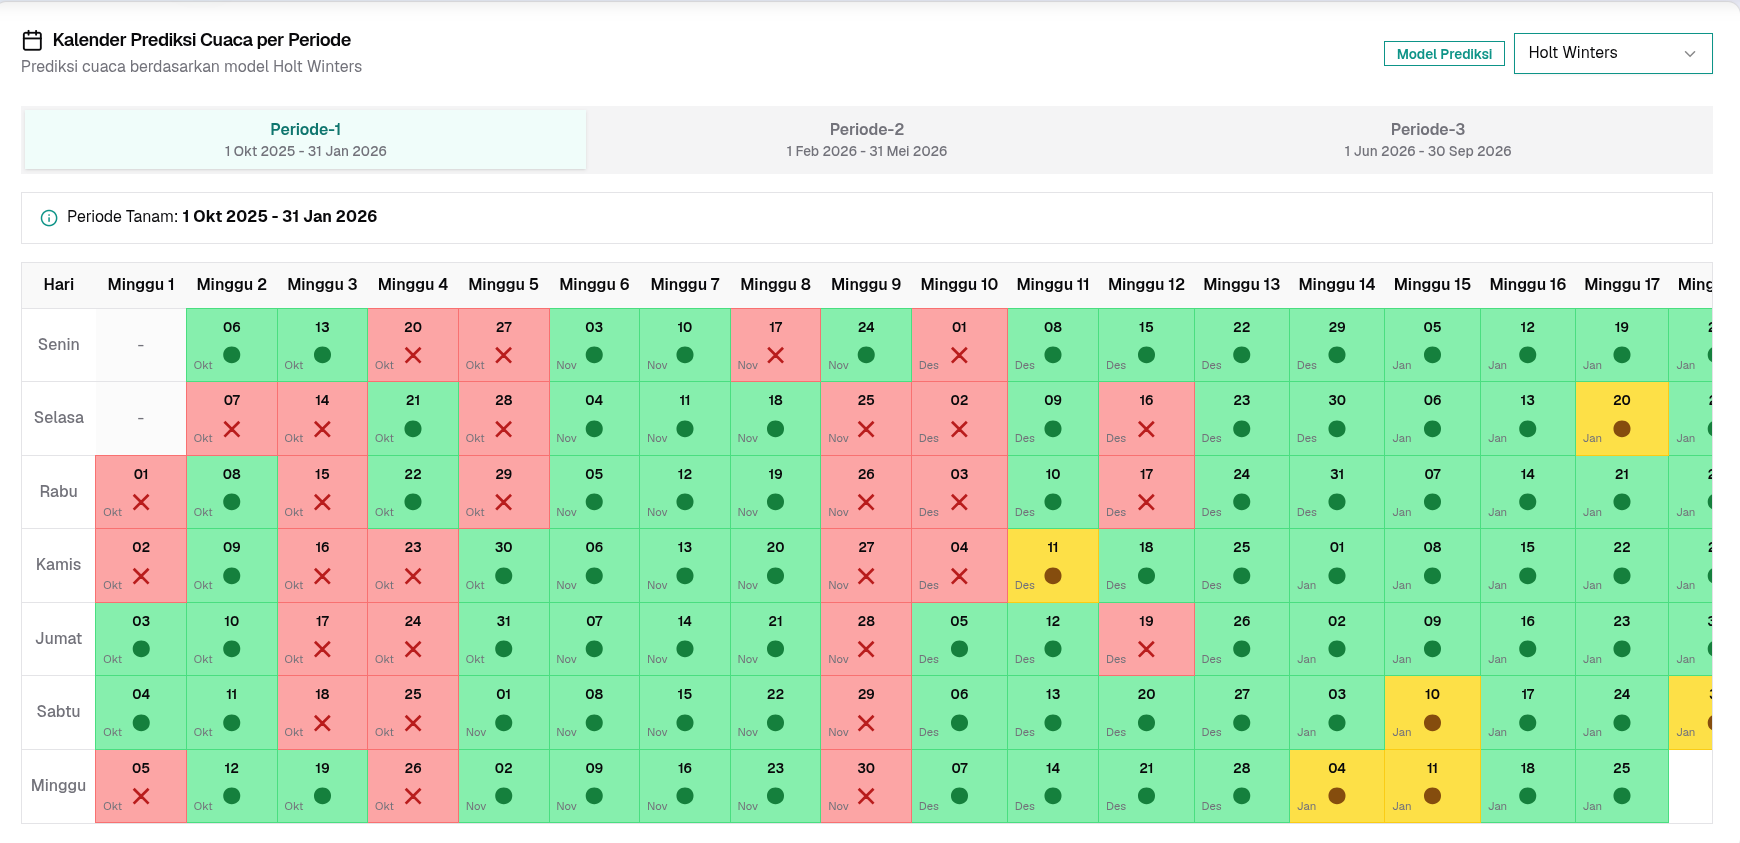
\includegraphics[width=0.8\linewidth]{image/bab4/kaltam/hw/kaltam_hw.png}
            \caption{Kalender Prediksi Cuaca Holt-Winters Periode 1 Oktober 2025 -- 30 September 2026}
            \label{fig:web_kaltam_hw}
    \end{figure}

Berdasarkan Gambar \ref{fig:web_kaltam_hw}, hasil peramalan metode \textit{Holt-Winters} menunjukkan bahwa periode tanam yang direkomendasikan terkonsentrasi pada 1 Oktober 2025 hingga 31 Januari 2026, di mana sebagian besar hari memenuhi kriteria kesesuaian iklim untuk budidaya padi sawah. Pada periode 1 Februari hingga 31 Mei 2026, jumlah hari yang sesuai mulai berkurang dan didominasi kategori waspada, meskipun masih terdapat beberapa hari yang layak untuk tanam pada awal Februari hingga pertengahan April. Selanjutnya, selama periode 1 Juni hingga 30 September 2026 seluruh hari dikategorikan sebagai tidak sesuai, sehingga direkomendasikan sebagai masa bera untuk persiapan musim tanam berikutnya.

Selain kalender tanam, sistem juga menyediakan fitur rekomendasi varietas padi berdasarkan durasi pertumbuhan. Fitur ini bertujuan membantu petani menyesuaikan waktu tanam dengan karakteristik masing-masing varietas, sehingga risiko kegagalan panen akibat kondisi iklim yang kurang mendukung dapat diminimalkan. Hasil prediksi durasi pertumbuhan varietas padi dari peramalan Holt-Winters ditampilkan pada Tabel \ref{tab:benih_hw}.
\begin{table}[H]
    \centering
    \caption{Prediksi Masa Tanam Varietas Padi Berdasarkan Hasil Peramalan Holt-Winters}
    \label{tab:benih_hw}
    \tiny
    \renewcommand{\arraystretch}{1.3}
    \setlength{\tabcolsep}{2pt}
    \begin{tabularx}{\textwidth}{|>{\raggedright\arraybackslash}X|>{\centering\arraybackslash}p{1.7cm}|>{\centering\arraybackslash}p{1.7cm}|>{\centering\arraybackslash}p{2.2cm}|>{\centering\arraybackslash}p{2.1cm}|>{\centering\arraybackslash}p{2.2cm}|>{\centering\arraybackslash}p{1.7cm}|}
        \hline
        \textbf{Varietas Padi} & \textbf{Durasi (Hari)} & \textbf{Lama Semai (Hari)} & \textbf{Tanggal Mulai Semai} & \textbf{Tanggal Tanam} & \textbf{Prediksi Panen} & \textbf{Sisa Waktu (Hari)} \\
        \hline
        Mustajab & 120 & 20 & 10 Okt 2025 & 30 Okt 2025 & 27 Feb 2026 & -21 \\
        \hline
        Ngawos & 95 & 20 & 10 Okt 2025 & 30 Okt 2025 & 2 Feb 2026 & 4 \\
        \hline
        Inpari 32 & 120 & 20 & 10 Okt 2025 & 30 Okt 2025 & 27 Feb 2026 & -21 \\
        \hline
        Ciherang & 125 & 20 & 10 Okt 2025 & 30 Okt 2025 & 4 Mar 2026 & -26 \\
        \hline
        Ciherang Beruang & 87 & 20 & 10 Okt 2025 & 30 Okt 2025 & 25 Jan 2026 & 12 \\
        \hline
        Cibatu & 100 & 20 & 10 Okt 2025 & 30 Okt 2025 & 7 Feb 2026 & -1 \\
        \hline
        Mekongga & 125 & 20 & 10 Okt 2025 & 30 Okt 2025 & 4 Mar 2026 & -26 \\
        \hline
        Ramos & 110 & 20 & 10 Okt 2025 & 30 Okt 2025 & 17 Feb 2026 & -11 \\
        \hline
        CBD 04 & 100 & 20 & 10 Okt 2025 & 30 Okt 2025 & 7 Feb 2026 & -1 \\
        \hline
        CBD Murni & 90 & 20 & 10 Okt 2025 & 30 Okt 2025 & 28 Jan 2026 & 9 \\
        \hline
        Beulerang & 150 & 20 & 10 Okt 2025 & 30 Okt 2025 & 29 Mar 2026 & -51 \\
        \hline
        Brangus & 150 & 20 & 10 Okt 2025 & 30 Okt 2025 & 29 Mar 2026 & -51 \\
        \hline
    \end{tabularx}
\end{table}
Berdasarkan hasil simulasi pada Tabel \ref{tab:benih_hw}, varietas dengan umur pendek seperti Ciherang Beruang (87 hari), CBD Murni (90 hari), dan Ngawos (95 hari) masih dapat dipanen sebelum berakhirnya periode tanam optimal dengan sisa waktu positif masing-masing 12, 9, dan 4 hari. Hal ini menunjukkan bahwa ketiga varietas tersebut relatif aman untuk ditanam pada tanggal 30 Oktober 2025 karena panen masih berada dalam rentang waktu yang direkomendasikan. 
Sebaliknya, varietas berumur sedang hingga panjang seperti Mustajab (120 hari), Inpari 32 (120 hari), Ciherang (125 hari), Mekongga (125 hari), Ramos (110 hari), Beulerang (150 hari), dan Brangus (150 hari) memiliki nilai sisa waktu negatif, yang berarti waktu panennya telah melewati periode tanam optimal. Kondisi ini berpotensi meningkatkan risiko penurunan produktivitas akibat curah hujan, suhu, kelembaban, atau radiasi matahari yang tidak lagi berada dalam kisaran ideal. 
Dengan demikian, metode Holt-Winters lebih sesuai digunakan untuk varietas padi berumur pendek, karena mampu meminimalkan risiko keterlambatan panen dan menjaga kesesuaian iklim selama fase pertumbuhan utama. Sementara itu, varietas berumur panjang memerlukan penyesuaian jadwal tanam yang lebih fleksibel agar tidak keluar dari periode tanam optimal.

\subsection{Analisis Metode LSTM}
Selanjutnya peramalan menggunakan metode LSTM diimplementasikan ke dalam kalender prediksi tanam untuk mengidentifikasi tingkat kesesuaian kondisi iklim. Adapun hasil peramalan LSTM untuk periode 1 Oktober 2025 hingga 30 September 2026 ditampilkan pada Tabel \ref{tab:kaltam_lstm} di bawah.
\begin{table}[H]
    \centering
    \caption{Kalender Tanam Kabupaten Aceh Besar Metode LSTM Periode Oktober 2025 -- September 2026}
    \label{tab:kaltam_lstm}
    \scriptsize
    \renewcommand{\arraystretch}{1.3}
    \setlength{\tabcolsep}{6pt}
    \begin{tabular}{|l|c|c|c|c|c|c|c|c|c|c|c|c|}
        \hline
        \textbf{Komoditas} & \textbf{Okt} & \textbf{Nov} & \textbf{Des} & \textbf{Jan} & \textbf{Feb} & \textbf{Mar} & \textbf{Apr} & \textbf{Mei} & \textbf{Jun} & \textbf{Jul} & \textbf{Agt} & \textbf{Sep} \\
        \hline
        Padi Sawah
        & \multicolumn{5}{c|}{\cellcolor{green!25}Tanam}
        & \multicolumn{3}{c|}{\cellcolor{yellow!30}Waspada}
        & \multicolumn{4}{c|}{\cellcolor{red!30}Bera}
        \\
        \hline
    \end{tabular}
\end{table}
Adapun hasil peramalan LSTM divisualisasikan dalam bentuk kalender prediksi cuaca sebagaimana ditunjukkan pada Gambar \ref{fig:web_kaltam_lstm}.

\begin{figure}[H]
    \centering
    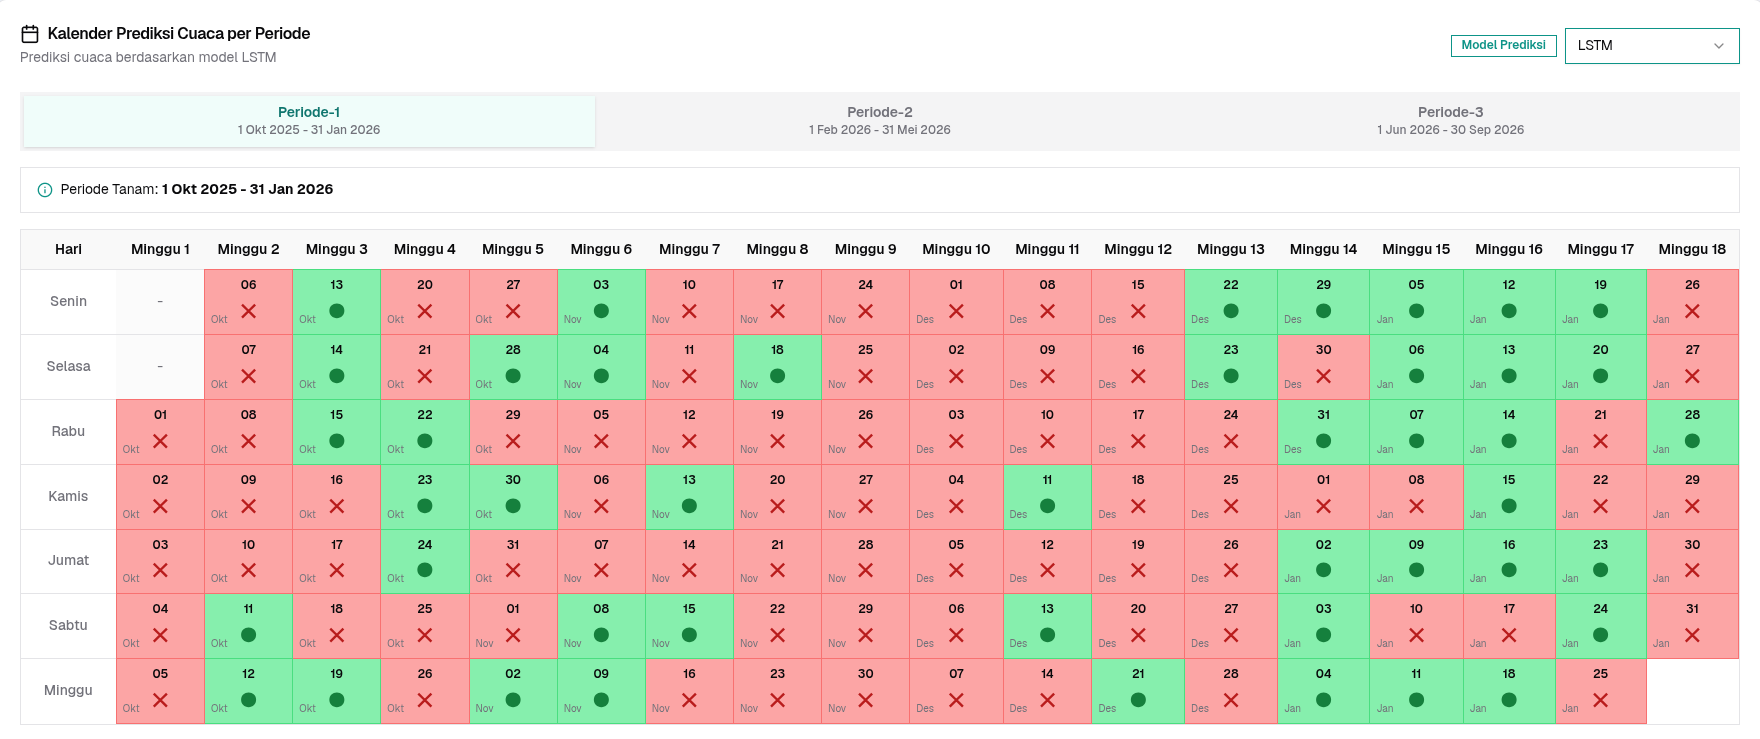
\includegraphics[width=0.8\linewidth]{image/bab4/kaltam/lstm/kaltam_lstm.png}
    \caption{Kalender Prediksi Cuaca LSTM Periode 1 Oktober 2025 -- 30 September 2026}
    \label{fig:web_kaltam_lstm}
\end{figure}

Berdasarkan Gambar \ref{fig:web_kaltam_lstm}, hasil peramalan metode LSTM menunjukkan bahwa periode tanam yang direkomendasikan berada pada rentang 1 Oktober 2025 hingga 31 Januari 2026. Selama periode tersebut masih terdapat banyak hari yang memenuhi kriteria kesesuaian iklim (indikasi hijau), meskipun diselingi beberapa hari tidak sesuai (indikasi merah), sehingga pemilihan waktu tanam perlu dilakukan secara selektif. Kondisi paling mendukung terlihat pada akhir Desember hingga pertengahan Januari, sedangkan setelah periode tersebut jumlah hari sesuai diperkirakan terus menurun sehingga risiko budidaya menjadi lebih tinggi.


\begin{table}[H]
    \centering
    \caption{Prediksi Masa Tanam Varietas Padi Berdasarkan Hasil Peramalan LSTM}
    \label{tab:benih_lstm}
    \tiny
    \renewcommand{\arraystretch}{1.3}
    \setlength{\tabcolsep}{2pt}
    \begin{tabularx}{\textwidth}{|>{\raggedright\arraybackslash}X|>{\centering\arraybackslash}p{1.7cm}|>{\centering\arraybackslash}p{1.7cm}|>{\centering\arraybackslash}p{2.2cm}|>{\centering\arraybackslash}p{2.1cm}|>{\centering\arraybackslash}p{2.2cm}|>{\centering\arraybackslash}p{1.7cm}|}
        \hline
        \textbf{Varietas Padi} & \textbf{Durasi (Hari)} & \textbf{Lama Semai (Hari)} & \textbf{Tanggal Mulai Semai} & \textbf{Tanggal Tanam} & \textbf{Prediksi Panen} & \textbf{Sisa Waktu (Hari)} \\
        \hline
        Mustajab & 120 & 20 & 10 Okt 2025 & 30 Okt 2025 & 27 Feb 2026 & -15 \\
        \hline
        Ngawos & 95 & 20 & 10 Okt 2025 & 30 Okt 2025 & 2 Feb 2026 & 11 \\
        \hline
        Inpari 32 & 120 & 20 & 10 Okt 2025 & 30 Okt 2025 & 27 Feb 2026 & -15 \\
        \hline
        Ciherang & 125 & 20 & 10 Okt 2025 & 30 Okt 2025 & 4 Mar 2026 & -20 \\
        \hline
        Ciherang Beruang & 87 & 20 & 10 Okt 2025 & 30 Okt 2025 & 25 Jan 2026 & 20 \\
        \hline
        Cibatu & 100 & 20 & 10 Okt 2025 & 30 Okt 2025 & 7 Feb 2026 & 7 \\
        \hline
        Mekongga & 125 & 20 & 10 Okt 2025 & 30 Okt 2025 & 4 Mar 2026 & -20 \\
        \hline
        Ramos & 110 & 20 & 10 Okt 2025 & 30 Okt 2025 & 17 Feb 2026 & -5 \\
        \hline
        CBD 04 & 100 & 20 & 10 Okt 2025 & 30 Okt 2025 & 7 Feb 2026 & 7 \\
        \hline
        CBD Murni & 90 & 20 & 10 Okt 2025 & 30 Okt 2025 & 28 Jan 2026 & 17 \\
        \hline
        Beulerang & 150 & 20 & 10 Okt 2025 & 30 Okt 2025 & 29 Mar 2026 & -44 \\
        \hline
        Brangus & 150 & 20 & 10 Okt 2025 & 30 Okt 2025 & 29 Mar 2026 & -44 \\
        \hline
    \end{tabularx}
\end{table}

Berdasarkan hasil simulasi pada Tabel \ref{tab:benih_lstm}, varietas dengan masa tumbuh pendek hingga sedang, seperti Ciherang Beruang, CBD Murni, Ngawos, dan Cibatu, menjadi varietas yang paling direkomendasikan karena masih memiliki sisa waktu panen yang relatif lebih besar dibandingkan varietas lainnya. Ciherang Beruang (87 hari) memiliki sisa waktu 20 hari, diikuti CBD Murni (90 hari) selama 17 hari, Ngawos (95 hari) selama 11 hari, dan Cibatu (100 hari) selama 7 hari. Kondisi tersebut menunjukkan bahwa varietas berumur pendek memiliki peluang lebih tinggi untuk dipanen sebelum memasuki periode iklim yang kurang mendukung.

Sebaliknya, varietas dengan masa tumbuh lebih panjang, seperti Mustajab, Inpari 32, Ciherang, Mekongga, Beulerang, dan Brangus, masih menunjukkan sisa waktu negatif sehingga berpotensi mengalami panen pada periode yang tidak lagi optimal. Meskipun demikian, dibandingkan hasil simulasi menggunakan metode Holt-Winters, metode LSTM memberikan sisa waktu yang umumnya lebih besar pada hampir seluruh varietas. Hal ini menunjukkan bahwa hasil peramalan LSTM mampu memberikan rekomendasi waktu tanam yang lebih adaptif terhadap kondisi iklim, sehingga menyediakan margin keamanan panen yang lebih baik bagi petani dalam menentukan varietas yang akan dibudidayakan.


\subsection{Perbandingan Hasil Kedua Metode}
Setelah dilakukan analisis kalender tanam berdasarkan hasil peramalan menggunakan metode Holt-Winters dan LSTM, tahap selanjutnya adalah membandingkan performa kedua metode berdasarkan metrik evaluasi. Perbandingan ini bertujuan untuk mengetahui metode yang menghasilkan tingkat kesalahan prediksi paling rendah sehingga dapat memberikan rekomendasi kalender tanam yang lebih akurat. Evaluasi dilakukan menggunakan tiga metrik, yaitu \textit{Mean Absolute Error} (MAE), \textit{Root Mean Square Error} (RMSE), dan \textit{Mean Absolute Percentage Error} (MAPE). Hasil perbandingan kedua metode ditunjukkan pada Tabel \ref{tab:eval_hw_lstm}.
\begin{table}[H]
    \centering
    \caption{Perbandingan Evaluasi Metrik Holt-Winters dan LSTM}
    \label{tab:eval_hw_lstm}
    \small
    \renewcommand{\arraystretch}{1.2}
    \setlength{\tabcolsep}{7pt}
    \begin{tabular}{|l|c|c|c|}
        \hline
        \textbf{Metode} & \textbf{MAE} & \textbf{RMSE} & \textbf{MAPE (\%)} \\
        \hline
        Holt-Winters & 5.65 & 13.71 & 60.83 \\
        \hline
        LSTM & \textbf{0.156} & \textbf{0.242} & \textbf{9.954} \\
        \hline
    \end{tabular}
\end{table}
Berdasarkan Tabel \ref{tab:eval_hw_lstm}, metode \textit{Long Short-Term Memory} (LSTM) menghasilkan performa prediksi yang lebih baik dibandingkan metode Holt-Winters pada seluruh metrik evaluasi. Nilai MAE LSTM sebesar 0.156 jauh lebih rendah dibandingkan Holt-Winters sebesar 5.65, menunjukkan bahwa rata-rata selisih antara nilai prediksi dan data aktual lebih kecil. Demikian pula nilai RMSE LSTM sebesar 0.242 lebih rendah daripada Holt-Winters sebesar 13.71, yang mengindikasikan kesalahan prediksi dengan deviasi besar dapat diminimalkan.

Perbedaan yang paling signifikan terlihat pada nilai MAPE. Metode LSTM memperoleh MAPE sebesar 9.954\%, sedangkan Holt-Winters mencapai 60.83\%. Berdasarkan kriteria interpretasi MAPE, nilai di bawah 10\% menunjukkan tingkat akurasi yang sangat baik, sedangkan nilai di atas 50\% menunjukkan akurasi prediksi yang rendah. Hasil tersebut menunjukkan bahwa LSTM mampu memodelkan pola data iklim yang bersifat nonlinier dan fluktuatif dengan lebih baik dibandingkan Holt-Winters yang lebih sesuai untuk data dengan pola musiman yang relatif stabil.

Temuan ini juga sejalan dengan hasil implementasi kalender tanam yang telah dibahas pada subbab sebelumnya. Kalender tanam berbasis LSTM memberikan rekomendasi periode tanam yang lebih adaptif terhadap perubahan kondisi iklim serta menyediakan margin waktu panen yang lebih baik pada sebagian besar varietas padi. Oleh karena itu, metode LSTM dinilai lebih sesuai untuk diimplementasikan sebagai model prediksi pada sistem kalender tanam yang dikembangkan dalam penelitian ini.

\begin{comment}
\end{comment}
